% =====================================================================
%  Bài toán nhiều electron trong phương trình Schrödinger
%  Biên dịch:  cd report && latexmk -xelatex bao_cao.tex
% =====================================================================
\documentclass[11pt,a4paper,oneside,openany]{report}

% ---------- Trang, phông chữ, ngôn ngữ ----------
\usepackage[a4paper,top=2.4cm,bottom=2.6cm,left=2.5cm,right=2.5cm,headheight=14pt]{geometry}
\usepackage{fontspec}
\usepackage{amsmath,amssymb}
\usepackage{unicode-math}
\setmainfont{TeX Gyre Pagella}
\setsansfont{Noto Sans}[Scale=MatchLowercase]
\setmonofont{Noto Sans Mono}[Scale=0.82]
\setmathfont{TeX Gyre Pagella Math}
\usepackage[vietnamese]{babel}
\usepackage{microtype}
\linespread{1.08}

% ---------- Màu ----------
\usepackage{xcolor}
\definecolor{cblue}{HTML}{257DE0}
\definecolor{corange}{HTML}{F47230}
\definecolor{caqua}{HTML}{00A888}
\definecolor{cviolet}{HTML}{6A4CE2}
\definecolor{cgreen}{HTML}{008A17}
\definecolor{cred}{HTML}{DC3C3D}
\definecolor{ctext}{HTML}{191919}
\definecolor{ctext2}{HTML}{555555}
\definecolor{bgblue}{HTML}{EAF2FC}
\definecolor{bggray}{HTML}{F4F4F4}
\definecolor{bgorange}{HTML}{FEF0E8}
\definecolor{bgaqua}{HTML}{E3F6F2}
\definecolor{bgviolet}{HTML}{F0EDFC}

% ---------- Hình, bảng, liên kết ----------
\usepackage{graphicx}
\graphicspath{{../figures/}}
\usepackage{booktabs,tabularx,multirow,array,longtable}
\usepackage{caption}
\captionsetup{font=small,labelfont={bf,sf},format=hang,justification=raggedright,singlelinecheck=false}
\usepackage{float}
\usepackage{enumitem}
\setlist{itemsep=2pt,topsep=4pt}
\usepackage{xurl}
\usepackage[hidelinks=false,colorlinks=true,linkcolor=cblue,citecolor=cviolet,urlcolor=cblue,
  pdftitle={Bài toán nhiều electron trong phương trình Schrödinger},
  pdfauthor={Kho Quantum-Physics}]{hyperref}

% ---------- Tiêu đề chương, đầu trang ----------
\usepackage{titlesec}
\titleformat{\chapter}[display]
  {\sffamily\bfseries\color{ctext}}
  {\color{cblue}\Large\MakeUppercase{\chaptertitlename}\ \thechapter}
  {6pt}{\Huge}
\titlespacing*{\chapter}{0pt}{-10pt}{22pt}
\titleformat{\section}{\sffamily\bfseries\Large\color{ctext}}{\color{cblue}\thesection}{0.7em}{}
\titleformat{\subsection}{\sffamily\bfseries\large\color{ctext}}{\color{cblue}\thesubsection}{0.6em}{}
\titleformat{\subsubsection}{\sffamily\bfseries\color{ctext}}{}{0em}{}
\usepackage{fancyhdr}
\pagestyle{fancy}
\fancyhf{}
\fancyhead[L]{\small\sffamily\color{ctext2}\nouppercase{\leftmark}}
\fancyfoot[C]{\small\sffamily\thepage}
\renewcommand{\headrulewidth}{0.4pt}
\renewcommand{\chaptermark}[1]{\markboth{\thechapter.\ #1}{}}
\fancypagestyle{plain}{\fancyhf{}\fancyfoot[C]{\small\sffamily\thepage}\renewcommand{\headrulewidth}{0pt}}

% ---------- Các hộp ----------
\usepackage[most]{tcolorbox}
\tcbset{
  hopchung/.style={breakable,enhanced,sharp corners,boxrule=0pt,leftrule=3pt,
    left=8pt,right=8pt,top=6pt,bottom=6pt,before skip=10pt,after skip=10pt,
    fonttitle=\sffamily\bfseries\small,coltitle=ctext,attach title to upper,
    after title={\par\smallskip}}
}
\newtcolorbox{eli5}[1][]{hopchung,colback=bgblue,colframe=cblue,
  title={\color{cblue}Hiểu nhanh (ELI5)\ifx&#1&\else: #1\fi}}
\newtcolorbox{congthuc}[1][]{hopchung,colback=bggray,colframe=ctext2,
  title={\color{ctext2}Công thức\ifx&#1&\else: #1\fi}}
\newtcolorbox{hieulam}[1][]{hopchung,colback=bgorange,colframe=corange,
  title={\color{corange}Hiểu lầm thường gặp\ifx&#1&\else: #1\fi}}
\newtcolorbox{chaycode}[1][]{hopchung,colback=bgaqua,colframe=caqua,
  title={\color{caqua}Chạy thử code\ifx&#1&\else: #1\fi}}
\newtcolorbox{ghinho}[1][]{hopchung,colback=bgviolet,colframe=cviolet,
  title={\color{cviolet}Ghi nhớ\ifx&#1&\else: #1\fi}}

% ---------- Ký hiệu tiện dùng ----------
\newcommand{\Ha}{\,\mathrm{Ha}}
\newcommand{\mHa}{\,\mathrm{mHa}}
\newcommand{\eV}{\,\mathrm{eV}}
\newcommand{\bohr}{\,\mathrm{bohr}}
\newcommand{\vr}{\mathbf r}
\newcommand{\vx}{\mathbf x}
\newcommand{\Hhat}{\hat H}
\newcommand{\Ecorr}{E_{\mathrm{corr}}}
\newcommand{\EHF}{E_{\mathrm{HF}}}
\newcommand{\code}[1]{\texttt{#1}}
\newcommand{\en}[1]{\textit{(#1)}}   % thuật ngữ tiếng Anh trong ngoặc

% Các con số tự sinh từ kết quả tính toán (code/06_tong_hop.py)
% Tự sinh bởi code/06_tong_hop.py - không sửa tay
\newcommand{\czeroSq}{0.9962}
\newcommand{\PctFciQZ}{96.3}
\newcommand{\ErrFciQZ}{+1.69}
\newcommand{\PctFciCBS}{99.7}
\newcommand{\ErrFciCBS}{+0.12}
\newcommand{\ErrMPtwoCBS}{+4.0}
\newcommand{\ErrCCSDTQZ}{+1.69}
\newcommand{\ErrCCSDTCBS}{+0.15}
\newcommand{\PctMPtwoQZ}{87}
\newcommand{\PctCorePVQZ}{38}
\newcommand{\PctCoreCVQZ}{96}
\newcommand{\ErrLDA}{+134}
\newcommand{\ErrPBE}{+16}
\newcommand{\ErrBLYP}{-5}
\newcommand{\ErrRtwoSCAN}{-1.6}
\newcommand{\ErrBthreeLYP}{-15}
\newcommand{\ErrPBEzero}{+11}
\newcommand{\HomoLDA}{3.16}
\newcommand{\HomoPBE}{3.23}
\newcommand{\HomoBthreeLYP}{3.65}
\newcommand{\HomoHF}{5.34}
\newcommand{\IEdeltaLDA}{5.47}
\newcommand{\IEdeltaPBE}{5.59}
\newcommand{\IEdeltaBthreeLYP}{5.63}
\newcommand{\HerrLDA}{+21.3}
\newcommand{\HerrPBE}{+0.02}
\newcommand{\HerrBthreeLYP}{-2.4}
\newcommand{\HerrHF}{+0.005}
\newcommand{\HhomoLDA}{7.3}
\newcommand{\HhomoPBE}{7.6}
\newcommand{\HhomoHF}{13.61}
\newcommand{\EvmcSlater}{-7.4182}
\newcommand{\PctVmcSlater}{-32}
\newcommand{\Evmc}{-7.4744}
\newcommand{\EvmcErr}{0.2}
\newcommand{\PctVmc}{92}
\newcommand{\ErrVmc}{+3.6}
\newcommand{\Edmc}{-7.47787}
\newcommand{\EdmcErr}{0.07}
\newcommand{\ErrDmc}{+0.19}
\newcommand{\PctDmc}{99.6}
\newcommand{\ZoneOpt}{2.28}
\newcommand{\ZtwoOpt}{0.61}


\begin{document}

% =====================================================================
\begin{titlepage}
\begin{center}
\vspace*{2.2cm}
{\sffamily\color{cblue}\large TÀI LIỆU TỰ HỌC\par}
\vspace{0.8cm}
{\sffamily\bfseries\fontsize{26}{32}\selectfont Bài toán nhiều electron\\[4pt] trong phương trình Schrödinger\par}
\vspace{0.7cm}
{\Large Từ nguyên tử liti đến các phương pháp giải hiện đại\par}
\vspace{0.5cm}
{\large\itshape Giải thích từ con số không, kèm code Python chạy được\par}
\vspace{1.6cm}
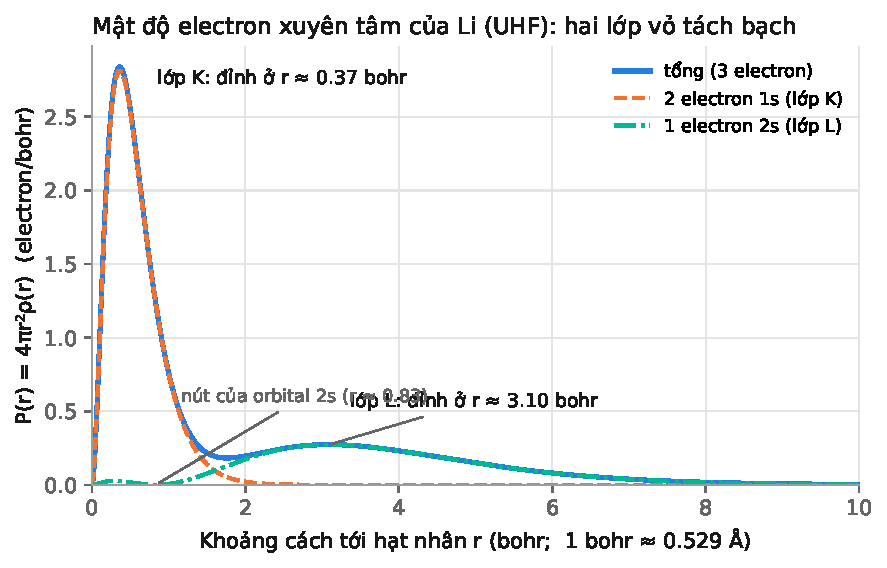
\includegraphics[width=0.62\textwidth]{02_mat_do_xuyen_tam.pdf}\par
\vspace{0.3cm}
{\small\color{ctext2}Mật độ electron của nguyên tử Li tính bằng code đi kèm: hai lớp vỏ 1s và 2s.\par}
\vfill
{\sffamily Kho \code{Quantum-Physics}\par}
\vspace{0.2cm}
{\sffamily\small Tháng 11/2026\par}
\vspace{0.2cm}
{\small\color{ctext2}Soạn với sự hỗ trợ của Claude (Anthropic): tìm tài liệu, viết code, chạy tính toán và viết bài.\\
Mọi con số trong tài liệu đều có nguồn hoặc được tính lại bằng code trong kho.\par}
\end{center}
\end{titlepage}

\pagenumbering{roman}
\tableofcontents
\clearpage
\pagenumbering{arabic}

\chapter*{Lời mở đầu}
\addcontentsline{toc}{chapter}{Lời mở đầu}
\markboth{Lời mở đầu}{}

Phương trình Schrödinger được viết ra năm 1926. Chỉ vài tháng sau, nó đã giải trọn vẹn nguyên tử hydro: một electron quay quanh một hạt nhân. Nhưng chỉ cần thêm \emph{một} electron (nguyên tử heli) là không còn công thức nghiệm nào nữa. Với liti (3 electron), cacbon (6 electron) hay một phân tử thuốc (hàng trăm electron), bài toán khó tới mức gần một thế kỷ sau, các nhà khoa học vẫn đang phát minh phương pháp mới để giải nó. Năm 1998, giải Nobel Hóa học được trao cho hai người đã nghĩ ra cách ``lách'' bài toán này: Walter Kohn (lý thuyết phiếm hàm mật độ) và John Pople (các phương pháp tính toán hóa lượng tử).

Tài liệu này kể lại câu chuyện đó cho người mới bắt đầu, với mục tiêu \textbf{hiểu sâu}: không chỉ biết tên các phương pháp, mà hiểu \emph{vì sao} bài toán khó, \emph{mỗi phương pháp xấp xỉ cái gì}, \emph{được gì và mất gì}.

\section*{Bạn cần biết gì trước khi đọc?}
Không nhiều. Bạn nên biết đạo hàm, tích phân, số phức ở mức cơ bản, và đã từng nghe về phương trình Schrödinger cho một hạt (giếng thế, nguyên tử hydro). Mọi khái niệm khác (spin, định thức Slater, phiếm hàm, Monte Carlo\ldots) đều được giải thích từ đầu. Đại số tuyến tính (ma trận, trị riêng) sẽ giúp ích nhiều ở chương 3 trở đi. Nếu chưa vững, Phụ lục~\ref{pl:lotrinh} có lộ trình học bổ sung.

\section*{Cách đọc tài liệu}
Mỗi khái niệm được trình bày theo hai lớp:
\begin{eli5}
Hộp màu xanh này giải thích ý tưởng bằng lời và ví dụ đời thường, không có công thức. Chỉ đọc các hộp xanh, bạn vẫn nắm được ``cốt truyện'' của cả tài liệu. Cuối mỗi ví dụ thường có một câu nói rõ ví dụ đó \emph{sai ở đâu}, vì mọi phép so sánh đều có giới hạn.
\end{eli5}
\begin{congthuc}
Hộp màu xám chứa công thức thật, kèm giải thích \emph{từng ký hiệu}. Đây là phần giúp bạn tự tính toán và đọc được sách chuyên ngành.
\end{congthuc}
\begin{hieulam}
Hộp màu cam chỉ ra những hiểu lầm mà người mới (và cả người không mới) hay mắc.
\end{hieulam}
\begin{chaycode}
Hộp màu xanh ngọc chỉ ra script Python trong thư mục \code{code/} tạo ra con số hoặc hình vẽ đang nói tới. Bạn có thể chạy lại, sửa tham số và tự quan sát.
\end{chaycode}
\begin{ghinho}
Hộp màu tím ở cuối mỗi chương tóm tắt những điều quan trọng nhất.
\end{ghinho}

\section*{Một nguyên tử xuyên suốt: liti}
Thay vì nói chung chung về ``hệ $N$ electron'', tài liệu dùng \textbf{nguyên tử liti} (Li, 3 electron) làm ví dụ xuyên suốt. Li là hệ nhỏ nhất có đủ mọi cái khó của bài toán nhiều electron: có lực đẩy giữa các electron, có nguyên lý Pauli buộc electron thứ ba phải lên lớp vỏ mới, có tương quan electron. Nhưng Li vẫn đủ nhỏ để một máy tính xách tay giải ``gần như chính xác'' bằng nhiều phương pháp, nên ta có thể \emph{so sánh} các phương pháp với một đáp án đã biết tới 15 chữ số:
\[
E_{\text{chính xác}}(\text{Li}) = -7.478\,060\,323\,910\Ha .
\]
Mọi phương pháp trong tài liệu (Hartree--Fock, CI, Coupled Cluster, DFT, Monte Carlo lượng tử) đều được chạy thật trên Li bằng code đi kèm, và kết quả được so với con số này.

\section*{Bản đồ tài liệu}
\begin{center}
\small
\begin{tabularx}{\textwidth}{@{}lX@{}}
\toprule
\textbf{Chương} & \textbf{Câu hỏi chính} \\
\midrule
1. Bài toán & Phương trình cho Li trông thế nào? Vì sao không giải được bằng công thức? \\
2. Hạt đồng nhất & Electron ``không có tên'' nghĩa là gì? Nguyên lý Pauli, định thức Slater, nguyên lý biến phân, năng lượng tương quan. \\
3. Hartree--Fock & Ý tưởng ``trường trung bình'': mỗi electron chỉ thấy đám mây trung bình của các electron khác. \\
4. Sau Hartree--Fock & Sửa phần thiếu của Hartree--Fock: CI, MP2, Coupled Cluster. \\
5. DFT & Bỏ hàm sóng $3N$ chiều, chỉ dùng mật độ electron 3 chiều. \\
6. Monte Carlo lượng tử & Giải bằng cách ``tung xúc xắc'' thông minh. \\
7. Biên giới & Mạng nơ-ron, máy tính lượng tử, mạng tensor. \\
8. Tổng kết & So sánh mọi phương pháp trên cùng một biểu đồ. \\
Phụ lục & Lộ trình tự học, tài liệu nên đọc, bảng thuật ngữ Việt--Anh, hướng dẫn chạy code. \\
\bottomrule
\end{tabularx}
\end{center}

\section*{Quy ước}
\begin{itemize}
\item \textbf{Đơn vị nguyên tử} (giải thích ở mục~\ref{sec:dvnt}): năng lượng tính bằng hartree (Ha), độ dài bằng bohr. $1\Ha = 27.211\eV$, $1\bohr = 0.529$\,Å. Ta thường dùng mHa (mili-hartree, $10^{-3}\Ha$).
\item \textbf{Dấu chấm thập phân} (7.478 chứ không phải 7,478), để khớp với code và với tài liệu quốc tế.
\item \textbf{Thuật ngữ}: dùng tiếng Việt, kèm thuật ngữ tiếng Anh trong ngoặc ở lần xuất hiện đầu, ví dụ: hàm sóng \en{wavefunction}. Bảng đầy đủ ở Phụ lục~\ref{pl:thuatngu}.
\item \textbf{Trích dẫn} dạng [số], danh sách ở cuối tài liệu, kèm DOI hoặc đường link.
\end{itemize}

\chapter{Bài toán: phương trình Schrödinger cho nhiều electron}
\label{ch:baitoan}

\section{Ôn nhanh: một electron thì dễ}

Với một hạt, phương trình Schrödinger dừng (không phụ thuộc thời gian) có dạng
\[
\Hhat\,\psi = E\,\psi .
\]
$\Hhat$ là \textbf{toán tử Hamilton} \en{Hamiltonian}, ``công thức tính năng lượng'' của hệ. $\psi$ là \textbf{hàm sóng} \en{wavefunction}. $E$ là năng lượng. Giải phương trình nghĩa là tìm những cặp $(E,\psi)$ thỏa mãn nó. Cặp có $E$ thấp nhất là \textbf{trạng thái cơ bản} \en{ground state}, trạng thái mà nguyên tử ở yên khi không bị kích thích. Mọi phương pháp trong tài liệu này đều nhắm tới trạng thái cơ bản.

Nguyên tử hydro (hoặc ion một electron có điện tích hạt nhân $Z$, như Li$^{2+}$) giải được chính xác: năng lượng các mức là
\[
E_n = -\frac{Z^2}{2n^2}\Ha, \qquad n = 1, 2, 3, \ldots
\]
Lý do là bài toán \textbf{tách biến} được: trong tọa độ cầu, hàm sóng là tích của một phần chỉ phụ thuộc bán kính và một phần chỉ phụ thuộc góc, $\psi = R_{nl}(r)\,Y_{lm}(\theta,\phi)$. Mỗi phần thỏa một phương trình một chiều giải được bằng tay \cite{Griffiths2018}. Với Li$^{2+}$ ($Z=3$, một electron): $E_1 = -9/2 = -4.5\Ha$, đúng tuyệt đối.

\section{Hamiltonian của nguyên tử nhiều electron}

\begin{eli5}[``hóa đơn năng lượng'']
Hamiltonian giống một \emph{hóa đơn năng lượng} của nguyên tử. Mỗi electron có một khoản ``tiền chạy'' (động năng, luôn dương) và một khoản ``thưởng'' vì được hạt nhân dương hút (thế năng hút, mang dấu âm). Mỗi \emph{cặp} electron phải trả thêm một khoản ``phí cãi nhau'' vì chúng đẩy nhau (thế năng đẩy, dương). Với Li có 3 electron: 3 khoản tiền chạy, 3 khoản thưởng, và 3 khoản phí cãi nhau (cặp 1--2, 1--3, 2--3), tổng cộng 9 khoản.

Cái khó nằm ở khoản ``phí cãi nhau'': số tiền mỗi electron phải trả \emph{phụ thuộc vào vị trí của các electron khác}. Không thể tính hóa đơn của từng electron riêng rẽ.
\end{eli5}

\begin{congthuc}[Hamiltonian trong hệ SI]
Nguyên tử có hạt nhân điện tích $Ze$ đặt cố định ở gốc tọa độ, $N$ electron:
\[
\Hhat=-\frac{\hbar^2}{2m_e}\sum_{i=1}^{N}\nabla_i^2
-\sum_{i=1}^{N}\frac{Ze^2}{4\pi\varepsilon_0\, r_i}
+\sum_{i<j}\frac{e^2}{4\pi\varepsilon_0\, r_{ij}}
\]
\begin{itemize}
\item $\hbar$: hằng số Planck rút gọn; $m_e$: khối lượng electron; $e$: điện tích nguyên tố; $\varepsilon_0$: hằng số điện của chân không.
\item $\nabla_i^2 = \partial^2/\partial x_i^2+\partial^2/\partial y_i^2+\partial^2/\partial z_i^2$: toán tử Laplace theo tọa độ $\vr_i$ của electron thứ $i$. Số hạng đầu là \textbf{động năng}.
\item $r_i = |\vr_i|$: khoảng cách từ electron $i$ tới hạt nhân. Số hạng thứ hai là \textbf{lực hút} electron--hạt nhân (dấu trừ: hút làm giảm năng lượng).
\item $r_{ij} = |\vr_i-\vr_j|$: khoảng cách giữa electron $i$ và $j$. Tổng $\sum_{i<j}$ chạy qua mọi cặp không lặp lại, gồm $N(N-1)/2$ số hạng. Đây là \textbf{lực đẩy} electron--electron.
\end{itemize}
\end{congthuc}

\subsection{Đơn vị nguyên tử}\label{sec:dvnt}
Các hằng số $\hbar, m_e, e, 4\pi\varepsilon_0$ xuất hiện khắp nơi và làm công thức rối mắt. Các nhà vật lý chọn một hệ đơn vị ``may đo'' cho nguyên tử, gọi là \textbf{đơn vị nguyên tử} \en{atomic units}, trong đó cả bốn hằng số này đều bằng 1. Giống như đo bàn học bằng gang tay thay vì mét: con số gọn hơn, còn bản chất không đổi.

\begin{congthuc}[đơn vị nguyên tử]
\begin{itemize}
\item Đơn vị độ dài: \textbf{bán kính Bohr} $a_0 = 4\pi\varepsilon_0\hbar^2/(m_e e^2) = 5.29177\times10^{-11}$\,m $\approx 0.529$\,Å, cỡ ``bán kính'' nguyên tử hydro.
\item Đơn vị năng lượng: \textbf{hartree}, $1\Ha = 27.211\,386\eV$ \cite{CODATA2022}. Năng lượng cơ bản của hydro là $-0.5\Ha$.
\item Quy đổi hữu ích: $1\eV = 0.036\,749\Ha$; $1$\,kcal/mol $= 1.594\mHa$.
\end{itemize}
Hamiltonian trở nên gọn gàng:
\[
\boxed{\;\Hhat=-\frac12\sum_{i=1}^{N}\nabla_i^2-\sum_{i=1}^{N}\frac{Z}{r_i}+\sum_{i<j}^{N}\frac{1}{r_{ij}}\;}
\]
Với Li ($Z=3$, $N=3$), viết tường minh cả 9 số hạng:
\[
\Hhat_{\rm Li}=\underbrace{-\tfrac12\nabla_1^2-\tfrac12\nabla_2^2-\tfrac12\nabla_3^2}_{\text{động năng}}
\;\underbrace{-\frac{3}{r_1}-\frac{3}{r_2}-\frac{3}{r_3}}_{\text{hút hạt nhân}}
\;\underbrace{+\frac{1}{r_{12}}+\frac{1}{r_{13}}+\frac{1}{r_{23}}}_{\text{đẩy nhau}}
\]
Phương trình cần giải là $\Hhat_{\rm Li}\,\Psi(\vr_1,\vr_2,\vr_3)=E\,\Psi(\vr_1,\vr_2,\vr_3)$, trong đó hàm sóng $\Psi$ phụ thuộc \emph{đồng thời} vào vị trí của cả ba electron: 9 biến số thực (chưa kể spin).
\end{congthuc}

Số số hạng tăng nhanh theo $N$: He có $2+2+1=5$ số hạng, Li có 9, C có 27, Fe ($N=26$) có $26+26+325=377$ số hạng. Phần đẩy nhau $N(N-1)/2$ tăng theo bình phương.

\subsection{Spin ở đâu?}
Hamiltonian trên \emph{không chứa spin}. Tuy vậy spin vẫn quyết định kết quả, qua nguyên lý Pauli mà chương~\ref{ch:hatdongnhat} sẽ trình bày. Đây là một trong những điều bất ngờ nhất của cơ học lượng tử: một tính chất không hề xuất hiện trong ``hóa đơn năng lượng'' lại quyết định cấu trúc của cả bảng tuần hoàn.

\section{Giả thiết hạt nhân đứng yên}

\begin{eli5}[con voi và đàn ruồi]
Hạt nhân $^7$Li nặng gấp khoảng \textbf{12\,786 lần} một electron. Hãy hình dung một con voi đứng giữa đàn ruồi: ruồi bay vù vù, còn con voi gần như không nhúc nhích. Vì vậy ta coi hạt nhân như bị ``đóng đinh'' ở gốc tọa độ và chỉ giải chuyển động của electron.
\end{eli5}

Với phân tử, ý tưởng này gọi là \textbf{gần đúng Born--Oppenheimer} \cite{BornOppenheimer1927}. Với nguyên tử, nó quy về giả thiết hạt nhân có khối lượng vô hạn. Sai số nhỏ cỡ nào? Puchalski và Pachucki \cite{PP2008} đã tính rất chính xác cho Li: hiệu chỉnh do hạt nhân có khối lượng hữu hạn là $+6.1\times10^{-4}\Ha$, còn hiệu chỉnh tương đối tính là $-6.4\times10^{-4}\Ha$. Cả hai đều cỡ $10^{-4}$ tương đối, và tình cờ gần như triệt tiêu nhau. Chúng nhỏ hơn 70 lần so với ``năng lượng tương quan'' ($0.045\Ha$, chương~\ref{ch:hatdongnhat}), đại lượng mà mọi phương pháp trong tài liệu này cố gắng tính. Vì thế từ đây ta chỉ xét bài toán \textbf{phi tương đối tính với hạt nhân cố định}. ``Năng lượng chính xác'' luôn được hiểu là nghiệm chính xác của bài toán này.

\section{Vì sao không giải được bằng công thức?}

\begin{eli5}[quả lắc và ba quả bóng nối lò xo]
Nguyên tử hydro giống một quả lắc treo vào cái đinh: chuyển động của nó tách được thành từng phần đơn giản (ra xa--lại gần, quay quanh), nên giải được trên giấy. Với Li, ba electron giống ba quả bóng nối với nhau bằng lò xo và cùng bị một nam châm hút. Cử động của quả này kéo theo hai quả kia, nên không thể chia việc cho từng quả rồi giải riêng.

Bài toán này giống bài toán \textbf{ba vật thể} nổi tiếng trong thiên văn (Mặt Trời--Trái Đất--Mặt Trăng): Poincaré chứng minh năm 1890 rằng nó không có thêm tích phân chuyển động nào để ``giải bằng công thức'' \cite{Poincare1890}; nghiệm tổng quát chỉ viết được dưới dạng một chuỗi vô hạn hội tụ cực chậm (Sundman, 1912).

\emph{Chỗ ví dụ ``gãy'':} trong lượng tử không có quỹ đạo, và phương trình Schrödinger là phương trình \emph{tuyến tính}, không hỗn loạn như cơ học thiên thể. Cái khó ở đây không phải hỗn loạn mà là các biến \emph{không tách rời được} và sống trong không gian quá nhiều chiều.
\end{eli5}

\begin{congthuc}[vì sao tách biến thất bại]
Nếu bỏ hết các số hạng đẩy $1/r_{ij}$, Hamiltonian tách thành tổng ba Hamiltonian kiểu hydro, mỗi cái chỉ chứa tọa độ của một electron:
\[
\Hhat^{(0)}=\hat h(1)+\hat h(2)+\hat h(3),\qquad \hat h(i)=-\tfrac12\nabla_i^2-\frac{Z}{r_i}.
\]
Khi đó nghiệm là tích $\Psi=\psi_a(\vr_1)\psi_b(\vr_2)\psi_c(\vr_3)$, với năng lượng bằng tổng năng lượng ba bài toán hydro. Ba electron chiếm 1s, 1s, 2s (chương~\ref{ch:hatdongnhat} sẽ giải thích vì sao):
\[
E^{(0)}=-\frac{9}{2}\Big(1+1+\frac14\Big)=-\frac{81}{8}=-10.125\Ha.
\]
Con số này sai tới 35\% so với $-7.478\Ha$. Lực đẩy giữa các electron không hề nhỏ! Nhưng khi giữ lại $1/r_{ij}=1/|\vr_i-\vr_j|$, số hạng này phụ thuộc \emph{đồng thời} vào hai electron, nên $\Psi$ không còn là tích các hàm một biến.
\end{congthuc}

Thậm chí với heli (2 electron), Fock đã chỉ ra năm 1954 rằng hàm sóng chính xác chứa các số hạng dạng logarit gần điểm hai electron cùng tiến về hạt nhân, tức là nó không phải hàm ``đẹp'' có thể viết bằng công thức sơ cấp \cite{Simon2018}.

\begin{hieulam}[``không có nghiệm giải tích'' = ``không biết đáp án'']
Sai! Không có \emph{công thức} không có nghĩa là không biết \emph{con số}. Năng lượng cơ bản của He đã được tính tới hơn 40 chữ số, của Li tới khoảng 15 chữ số, bằng các phương pháp biến phân số rất tinh xảo (bảng~\ref{tab:chuso}). Điều khó là \emph{chi phí} tăng vọt khi thêm electron: từ He sang Li, lượng tính toán cần để đạt độ chính xác phổ học tăng khoảng 6000 lần \cite{Ruiz2021}.
\end{hieulam}

\begin{table}[h]
\centering\small
\caption{Năng lượng phi tương đối tính tốt nhất hiện nay cho vài nguyên tử nhẹ. Mỗi electron thêm vào làm mất vài chữ số chính xác.}
\label{tab:chuso}
\begin{tabular}{@{}clrcl@{}}
\toprule
$N$ & Nguyên tử & Năng lượng tốt nhất (Ha) & Số chữ số & Nguồn \\
\midrule
2 & He & $-2.903\,724\,377\,034\,119\,598\ldots$ & $>40$ & \cite{Nakashima2007,Schwartz2006} \\
3 & Li & $-7.478\,060\,323\,910\,147(1)$ & $\sim15$ & \cite{Wang2012,PKP2009} \\
4 & Be & $-14.667\,356\,508(1)$ & $\sim11$ & \cite{Hornyak2019} \\
6 & C & $-37.844\,906(4)$ & $\sim7$ & \cite{Strasburger2019} \\
\bottomrule
\end{tabular}
\end{table}

\section{Bức tường hàm mũ}\label{sec:buctuong}

\begin{eli5}[bản đồ xác suất]
Muốn ghi lại ``bản đồ xác suất'' của \emph{một} electron, ta chia không gian quanh nguyên tử thành lưới $10\times10\times10 = 1000$ ô và ghi một con số vào mỗi ô. Với \emph{ba} electron, bản đồ phải trả lời câu hỏi ``electron 1 ở ô này \emph{và} electron 2 ở ô kia \emph{và} electron 3 ở ô nọ'' cho \emph{mọi} tổ hợp: $1000\times1000\times1000=10^9$ con số, khoảng 8\,GB, vừa đủ cho một chiếc laptop. Cacbon (6 electron) cần $10^{18}$ con số, khoảng 8 exabyte. Sắt (26 electron) cần $10^{78}$ con số, \emph{ngang số nguyên tử trong vũ trụ quan sát được}. Mỗi electron thêm vào nhân kích thước lên 1000 lần: đó là ``bức tường''.

\emph{Chỗ ví dụ ``gãy'':} hàm sóng thật mượt và có đối xứng, nên không cần ghi ``mọi tổ hợp'' một cách ngây thơ. Các phương pháp thông minh trong những chương sau khai thác đúng điều này.
\end{eli5}

\begin{figure}[h]
\centering
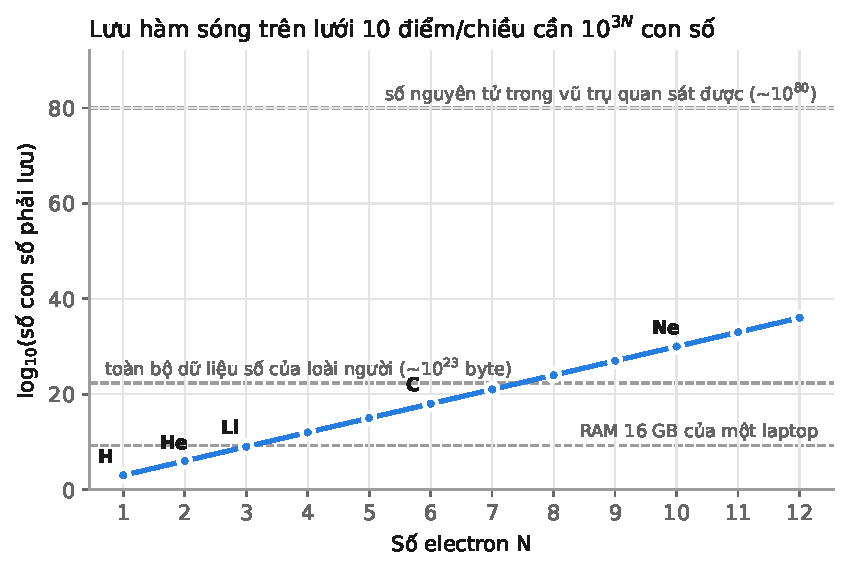
\includegraphics[width=0.86\textwidth]{01_buc_tuong_ham_mu.pdf}
\caption{Số con số cần lưu để ghi hàm sóng của $N$ electron trên lưới 10 điểm mỗi chiều: $10^{3N}$. Trục tung dùng thang log nên đường thẳng nghĩa là tăng theo hàm mũ. Ba vạch ngang là RAM laptop, toàn bộ dữ liệu số của loài người, và số nguyên tử trong vũ trụ. (Script \code{01\_nen\_tang.py})}
\label{fig:buctuong}
\end{figure}

Walter Kohn gọi hiện tượng này là \textbf{bức tường hàm mũ} \en{exponential wall} trong bài giảng nhận giải Nobel năm 1998 \cite{Kohn1999}. Lập luận của ông: để năng lượng chính xác cỡ 1\%, mỗi tọa độ cần khoảng $p = 3$ đến $10$ tham số, nên tổng số tham số là
\[
M = p^{3N}.
\]
Nếu máy tính tốt nhất xử lý được $\bar M\approx10^9$ tham số với $p=3$, thì số electron tối đa là $\bar N = \frac13\log_{10}\bar M/\log_{10} p\approx 6$. Kohn viết: \emph{``Let us optimistically take $\bar M\approx10^9$ and $p=3$. This gives the shocking result $\bar N=\frac13\cdot\frac{9}{0.48}=6$ (!)''}, và \emph{``the exponential in Eq.~(2.12) represents a `wall' severely limiting $\bar N$''}. Với 100 electron, $M\approx3^{300}\approx10^{143}$, một con số không có ý nghĩa thực tế nào.

Bức tường không chỉ xuất hiện khi dùng lưới. Chương~\ref{ch:sauhf} sẽ cho thấy cách viết hàm sóng bằng tổ hợp các ``cấu hình electron'' (Full CI) cũng gặp đúng bức tường này dưới dạng tổ hợp.

\section{Câu nói của Dirac}

Năm 1929, chỉ ba năm sau phương trình Schrödinger, Paul Dirac viết một câu đã trở thành ``tuyên ngôn'' của ngành hóa học tính toán \cite{Dirac1929}:

\begin{quote}
\itshape ``The underlying physical laws necessary for the mathematical theory of a large part of physics and the whole of chemistry are thus completely known, and the difficulty is only that the exact application of these laws leads to equations much too complicated to be soluble. It therefore becomes desirable that approximate practical methods of applying quantum mechanics should be developed\ldots''
\end{quote}
Tạm dịch: \emph{Các định luật vật lý nền tảng cho phần lớn vật lý và toàn bộ hóa học đã được biết đầy đủ. Cái khó chỉ là việc áp dụng chính xác các định luật này dẫn tới những phương trình quá phức tạp để giải được. Vì vậy cần phát triển các phương pháp gần đúng thực tế\ldots}

Toàn bộ phần còn lại của tài liệu là câu chuyện về các ``phương pháp gần đúng thực tế'' đó.

\begin{ghinho}
\begin{itemize}
\item Hamiltonian của nguyên tử $N$ electron gồm động năng, hút hạt nhân, và $N(N-1)/2$ số hạng đẩy nhau $1/r_{ij}$. Chính các số hạng đẩy nhau làm bài toán không tách biến được.
\item Bỏ lực đẩy, Li cho $-10.125\Ha$ (sai 35\%). Lực đẩy không phải ``hiệu chỉnh nhỏ''.
\item Hàm sóng $N$ electron sống trong không gian $3N$ chiều. Lưu nó một cách ngây thơ cần $\sim10^{3N}$ con số: bức tường hàm mũ.
\item ``Không có công thức'' khác ``không biết đáp án'': năng lượng Li đã biết tới 15 chữ số, $-7.478\,060\,323\,910\Ha$. Ta sẽ dùng con số này làm trọng tài cho mọi phương pháp.
\end{itemize}
\end{ghinho}

\chapter{Hạt đồng nhất, nguyên lý biến phân và năng lượng tương quan}
\label{ch:hatdongnhat}

Chương này trang bị ba công cụ mà mọi phương pháp sau đều dùng: (1) quy tắc phản đối xứng của electron, dẫn tới nguyên lý Pauli và định thức Slater; (2) nguyên lý biến phân, ``la bàn'' cho biết một hàm sóng gần đúng tốt hay dở; (3) khái niệm năng lượng tương quan, thước đo cho phần khó nhất của bài toán.

\section{Electron không có tên}

\begin{eli5}[tiền trong tài khoản]
Bạn có hai tờ 100 nghìn trong tài khoản ngân hàng. Không có ``tờ thứ nhất'' hay ``tờ thứ hai'', chỉ có ``200 nghìn''. Electron cũng vậy: mọi electron giống hệt nhau, \textbf{không thể dán nhãn}. Nếu đổi chỗ hai electron, không thí nghiệm nào phân biệt được trước và sau.

Riêng electron còn có một quy tắc kỳ lạ: khi đổi chỗ hai electron trong công thức, hàm sóng \textbf{đổi dấu} (nhân với $-1$), còn xác suất (bình phương của hàm sóng) thì không đổi.

\emph{Chỗ ví dụ ``gãy'':} tiền không có ``dấu trừ khi đổi chỗ''. Quy tắc đổi dấu của electron không có tương tự nào trong đời thường.
\end{eli5}

\begin{congthuc}[tính phản đối xứng]
Ghép vị trí $\vr$ và spin $\omega$ (``lên'' $\uparrow$ hoặc ``xuống'' $\downarrow$) của electron thành một biến $\vx=(\vr,\omega)$. Hàm sóng của mọi hệ electron phải thỏa
\[
\Psi(\ldots,\vx_i,\ldots,\vx_j,\ldots)=-\,\Psi(\ldots,\vx_j,\ldots,\vx_i,\ldots)\qquad\text{với mọi cặp } i,j.
\]
Hamiltonian đối xứng với mọi phép đổi nhãn, nhưng yêu cầu phản đối xứng \emph{không} suy ra được từ đó. Nó là một tiên đề mới của cơ học lượng tử, đứng ngang hàng về mặt logic với chính phương trình Schrödinger \cite{Griffiths2018}. Những hạt tuân theo quy tắc này gọi là \textbf{fermion} (electron, proton, neutron); hạt có hàm sóng đối xứng (không đổi dấu) gọi là \textbf{boson} (photon, nguyên tử $^4$He).
\end{congthuc}

\section{Spin và nguyên lý loại trừ Pauli}

\begin{eli5}[rạp chiếu phim]
Hình dung các \emph{orbital} (vùng không gian mà electron hay có mặt) như các hàng ghế trong rạp chiếu phim. Mỗi hàng chỉ có đúng hai ghế: một ghế ``spin lên'', một ghế ``spin xuống''. Không bao giờ có hai electron ngồi cùng một ghế: đó là \textbf{nguyên lý loại trừ Pauli} \cite{Pauli1925}. Li có 3 electron. Hai người đầu ngồi kín hàng 1s (một lên, một xuống), người thứ ba buộc phải lên hàng sau, hàng 2s.

\emph{Chỗ ví dụ ``gãy'':} electron không ``ngồi'' ở đâu cả; orbital chỉ là công cụ gần đúng; và ``spin lên/xuống'' không phải electron tự quay như con quay.
\end{eli5}

Nguyên lý Pauli không phải là một quy tắc thêm vào, mà là \emph{hệ quả} của tính phản đối xứng. Để thấy điều đó, ta cần một cách viết hàm sóng tự động phản đối xứng: định thức Slater.

\section{Định thức Slater}

Cách đơn giản nhất để tạo hàm sóng nhiều electron là nhân các hàm một electron: $\Psi=\chi_1(\vx_1)\chi_2(\vx_2)\chi_3(\vx_3)$, gọi là \textbf{tích Hartree} \en{Hartree product}. Mỗi $\chi$ là một \textbf{spin-orbital}: tích của một orbital không gian $\varphi(\vr)$ và một hàm spin $\alpha$ ($\uparrow$) hoặc $\beta$ ($\downarrow$). Nhưng tích Hartree ``dán nhãn'' electron (electron 1 ở $\chi_1$\ldots) và không đổi dấu khi đổi chỗ, nên vi phạm tiên đề trên. Slater (1929) nhận ra rằng \textbf{định thức} của ma trận có tính chất đúng như ta cần \cite{Slater1929}: đổi hai hàng thì định thức đổi dấu.

\begin{congthuc}[định thức Slater cho Li]
Đặt $a=\varphi_{1s}\alpha$ (1s, spin lên), $b=\varphi_{1s}\beta$ (1s, spin xuống), $c=\varphi_{2s}\alpha$ (2s, spin lên). Hàng $i$ ứng với electron $i$, cột ứng với spin-orbital:
\[
\Psi_{\rm Li}(\vx_1,\vx_2,\vx_3)=\frac{1}{\sqrt{3!}}
\begin{vmatrix}
a(\vx_1) & b(\vx_1) & c(\vx_1)\\
a(\vx_2) & b(\vx_2) & c(\vx_2)\\
a(\vx_3) & b(\vx_3) & c(\vx_3)
\end{vmatrix}
\]
Khai triển ra đủ $3!=6$ số hạng:
\[
\Psi_{\rm Li}=\tfrac{1}{\sqrt6}\big[a_1b_2c_3-a_1c_2b_3-b_1a_2c_3+b_1c_2a_3+c_1a_2b_3-c_1b_2a_3\big],
\]
với $a_1$ là viết tắt của $a(\vx_1)$. Hệ số $1/\sqrt{6}$ để hàm sóng chuẩn hóa.

Ba tính chất của định thức cho ra ba định luật vật lý:
\begin{itemize}
\item \textbf{Đổi hai hàng} (đổi chỗ hai electron) thì định thức đổi dấu: đúng tiên đề phản đối xứng.
\item \textbf{Hai cột giống nhau} (hai electron cùng spin-orbital) thì định thức bằng 0: đó chính là \textbf{nguyên lý Pauli}. Thử nhét cả ba electron vào 1s: $a, b, a$ có cột 1 và 3 trùng nhau, nên $\Psi\equiv0$. Cấu hình 1s$^3$ không tồn tại.
\item \textbf{Hai hàng giống nhau} (hai electron cùng spin ở cùng một điểm) thì định thức bằng 0: hai electron cùng spin không bao giờ gặp nhau. Quanh mỗi electron có một ``vùng cấm'' với các electron cùng spin, gọi là \textbf{lỗ Fermi} \en{Fermi hole}.
\end{itemize}
\end{congthuc}

\begin{hieulam}[``electron số 3 là electron 2s'']
Trong định thức Slater, \emph{mọi} electron xuất hiện trong \emph{mọi} spin-orbital (nhìn 6 số hạng ở trên: electron 1 có lúc ở $a$, lúc ở $b$, lúc ở $c$). Câu ``Li có hai electron 1s và một electron 2s'' chỉ là cách nói tắt cho ``định thức được dựng từ các spin-orbital 1s$\uparrow$, 1s$\downarrow$, 2s$\uparrow$''.
\end{hieulam}

\begin{hieulam}[``nguyên lý Pauli là một lực đẩy'']
Không có lực nào cả. Electron cùng spin ``tránh nhau'' vì một ràng buộc thuần túy hình học của tính phản đối xứng. Griffiths viết về ``lực trao đổi'': \emph{``it's not really a force at all --- no physical agency is pushing on the particles; rather, it is a purely geometrical consequence of the symmetrization requirement''} \cite{Griffiths2018}.
\end{hieulam}

\subsection{Vì sao electron thứ ba vào 2s mà không vào 2p?}
Pauli chỉ nói 1s đã đầy. Còn việc chọn 2s thay vì 2p là hiệu ứng của lực đẩy giữa các electron. Trong hydro, 2s và 2p có cùng năng lượng. Trong Li, 2p cao hơn 2s tới $1.848\eV$; đó chính là vạch đỏ 671\,nm làm ngọn lửa muối liti có màu đỏ son \cite{NIST-ASD}. Nguyên nhân là orbital 2s có một phần nhỏ ``xuyên'' vào sát hạt nhân, bên trong lớp 1s, nên bị hai electron 1s \textbf{che chắn} \en{screening} ít hơn. Electron 2p gần như chỉ ``thấy'' điện tích $+1$ (hạt nhân $+3$ bị hai electron 1s che mất $-2$), còn electron 2s thấy khoảng $+1.26$.

Hình~\ref{fig:matdo} (tính bằng code của chương~\ref{ch:hf}) cho thấy rõ cấu trúc lớp vỏ: hai electron 1s tập trung rất gần hạt nhân (đỉnh ở $r\approx0.36\bohr$), electron 2s nằm xa hơn gần 9 lần (đỉnh ở $r\approx3.1\bohr$), nhưng vẫn có một ``thùy'' nhỏ bên trong lớp 1s, ngăn cách bởi một \textbf{nút} \en{node} tại $r\approx0.83\bohr$.

\begin{figure}[h]
\centering
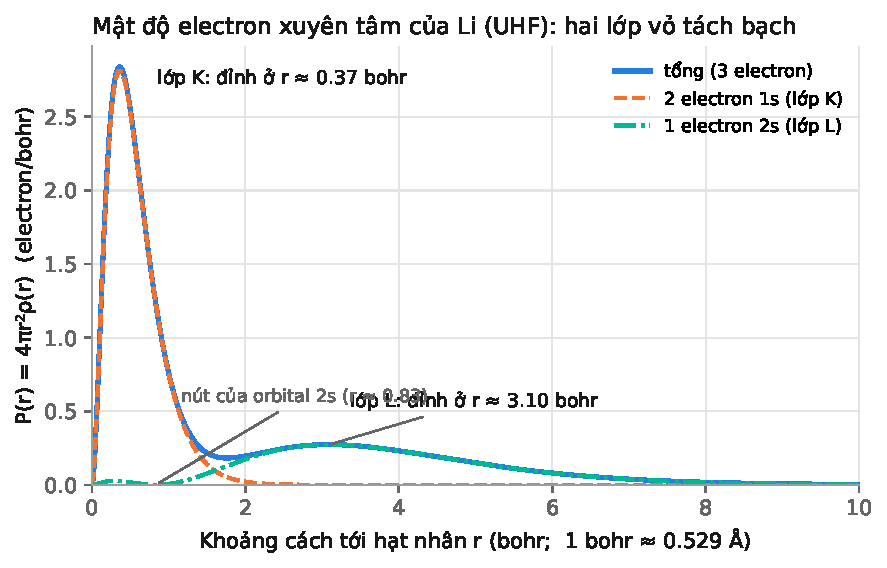
\includegraphics[width=0.8\textwidth]{02_mat_do_xuyen_tam.pdf}
\caption{Mật độ electron xuyên tâm $P(r)=4\pi r^2\rho(r)$ của Li (Hartree--Fock không hạn chế, tập cơ sở aug-cc-pCVQZ). Diện tích dưới đường tổng bằng đúng 3 electron. Thùy nhỏ của 2s bên trong lớp 1s là phần ``xuyên thấu'' giúp 2s có năng lượng thấp hơn 2p. (Script \code{02\_hartree\_fock.py})}
\label{fig:matdo}
\end{figure}

\subsection{Spin toàn phần: Li là một ``doublet''}
Hai electron 1s có spin ngược nhau nên tổng spin của cặp bằng 0. Electron 2s không có cặp, nên spin toàn phần của Li là $S=\tfrac12$ và có $2S+1=2$ cách định hướng: trạng thái \textbf{doublet}, ký hiệu $1s^22s\;{}^2S_{1/2}$. Vì có một electron lẻ, Li thuộc loại hệ \textbf{vỏ mở} \en{open-shell}. Chương~\ref{ch:hf} sẽ cho thấy điều này đòi hỏi hai biến thể của phương pháp Hartree--Fock (ROHF và UHF).

\section{Nguyên lý biến phân}\label{sec:bienphan}

\begin{eli5}[tìm đáy thung lũng trong sương mù]
Bạn phải tìm điểm thấp nhất của một thung lũng chìm trong sương mù. Bạn không nhìn thấy đáy, nhưng biết chắc một điều: \emph{mọi chỗ bạn đứng đều cao hơn hoặc bằng đáy}. Đi thử nhiều chỗ, chỗ thấp nhất bạn tìm được luôn là một ``cận trên'' của độ sâu thật. Đi càng khéo, càng gần đáy.

Trong lượng tử, ``chỗ đứng'' là một hàm sóng đoán thử, còn ``độ cao'' là năng lượng tính từ hàm đó. Năng lượng của hàm đoán thử không bao giờ thấp hơn năng lượng cơ bản thật.

\emph{Chỗ ví dụ ``gãy'':} ``thung lũng'' ở đây nằm trong một không gian vô hạn chiều (không gian các hàm), và bạn phải đi đúng ``lối'' (hàm phản đối xứng). Đi sai lối có thể rơi xuống một thung lũng ``cấm'' sâu hơn đáy thật, như sẽ thấy ở hình~\ref{fig:bacthang}.
\end{eli5}

\begin{congthuc}[định lý biến phân]
Với mọi hàm thử $\Phi$ có đúng tính đối xứng (phản đối xứng với electron),
\[
E[\Phi]=\frac{\langle\Phi|\Hhat|\Phi\rangle}{\langle\Phi|\Phi\rangle}\;\ge\;E_0 ,
\]
dấu bằng xảy ra khi và chỉ khi $\Phi$ là hàm sóng cơ bản. Ở đây $\langle\Phi|\Hhat|\Phi\rangle=\int\Phi^*\,\Hhat\,\Phi\,d\tau$ là tích phân trên mọi tọa độ và spin.

\textbf{Chứng minh (3 dòng).} Khai triển $\Phi=\sum_n c_n\Psi_n$ theo các trạng thái riêng chính xác $\Hhat\Psi_n=E_n\Psi_n$ (chúng tạo thành một cơ sở trực chuẩn). Khi đó
\[
E[\Phi]=\frac{\sum_n|c_n|^2E_n}{\sum_n|c_n|^2}\;\ge\;\frac{\sum_n|c_n|^2E_0}{\sum_n|c_n|^2}=E_0 ,
\]
vì mọi $E_n\ge E_0$. Năng lượng của hàm thử là một trung bình có trọng số của các $E_n$, và trung bình không thể nhỏ hơn số nhỏ nhất.

\textbf{Một hệ quả dễ chịu.} Nếu hàm thử sai lệch cỡ $\epsilon$ so với hàm đúng, năng lượng chỉ sai lệch cỡ $\epsilon^2$. Hàm sóng sai 10\% thì năng lượng chỉ sai cỡ 1\%. Vì thế năng lượng thường tốt hơn nhiều so với hàm sóng tạo ra nó. Ngược lại, năng lượng tốt chưa chắc các tính chất khác (như mật độ ở sát hạt nhân) cũng tốt.
\end{congthuc}

Gần như mọi phương pháp trong tài liệu này dựa trên nguyên lý biến phân: Hartree--Fock, CI, Monte Carlo biến phân, mạng nơ-ron. Hai ngoại lệ quan trọng là MP2 và Coupled Cluster (chương~\ref{ch:sauhf}): chúng \emph{không} cho cận trên.

\subsection{Ví dụ khởi động: nguyên tử heli}
Thử hàm $\Phi=e^{-\zeta(r_1+r_2)}$: cả hai electron ở orbital kiểu 1s, nhưng thay điện tích hạt nhân thật $Z=2$ bằng một ``điện tích hiệu dụng'' $\zeta$ có thể điều chỉnh. (Với hai electron spin ngược nhau, phần không gian đối xứng; tính phản đối xứng nằm trong phần spin.) Tính các tích phân (xem \cite{Griffiths2018}, chương 8) cho:
\[
E(\zeta)=\underbrace{\zeta^2}_{\text{động năng}}\;\underbrace{-\,2Z\zeta}_{\text{hút hạt nhân}}\;+\;\underbrace{\tfrac58\zeta}_{\text{đẩy nhau}} .
\]
Đạo hàm bằng 0 cho $\zeta^*=Z-\tfrac{5}{16}=\tfrac{27}{16}=1.6875$ và $E(\zeta^*)=-(27/16)^2=-2.8477\Ha$, cao hơn giá trị chính xác $-2.9037\Ha$ đúng như định lý khẳng định (hình~\ref{fig:he}). Ý nghĩa vật lý: $\zeta^*<Z$, vì mỗi electron bị electron kia \textbf{che chắn} một phần điện tích hạt nhân.

\begin{figure}[h]
\centering
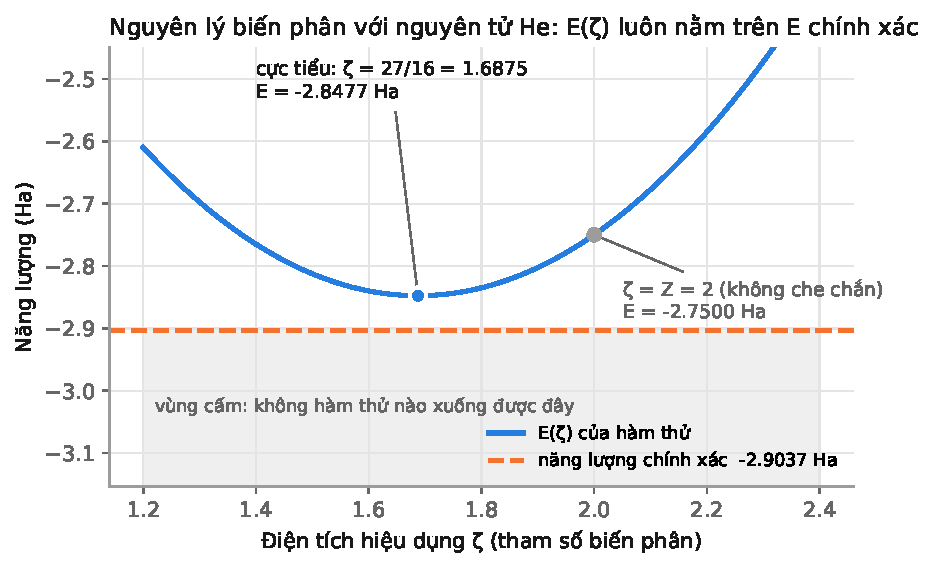
\includegraphics[width=0.78\textwidth]{01_bien_phan_he.pdf}
\caption{Nguyên lý biến phân với nguyên tử He. Mọi giá trị của tham số $\zeta$ cho năng lượng cao hơn đáp án chính xác (vạch cam). Giá trị tốt nhất $\zeta^*=27/16$ vẫn sai $56\mHa$. (Script \code{01\_nen\_tang.py})}
\label{fig:he}
\end{figure}

\subsection{Áp dụng cho Li: bậc thang năng lượng}
Với Li, dùng định thức $|1s\!\uparrow 1s\!\downarrow 2s\!\uparrow|$ với các orbital kiểu hydro có chung điện tích hiệu dụng $\zeta$. Tính các tích phân theo quy tắc Slater--Condon \cite{Szabo1996} được
\[
E(\zeta)=\tfrac98\zeta^2-\tfrac{27}{4}\zeta+\Big(\underbrace{\tfrac58}_{J_{1s1s}}+\underbrace{\tfrac{34}{81}}_{2J_{1s2s}}-\underbrace{\tfrac{16}{729}}_{K_{1s2s}}\Big)\zeta ,
\]
cực tiểu tại $\zeta^*=2.5454$ với $E=-7.2891\Ha$. Số hạng $K_{1s2s}$ mang dấu trừ là \textbf{năng lượng trao đổi} \en{exchange energy}: nó chỉ xuất hiện giữa hai electron \emph{cùng spin} (1s$\uparrow$ và 2s$\uparrow$) và là ``dấu vết'' năng lượng của lỗ Fermi. Chương~\ref{ch:hf} sẽ nói kỹ về $J$ và $K$.

\begin{figure}[h]
\centering
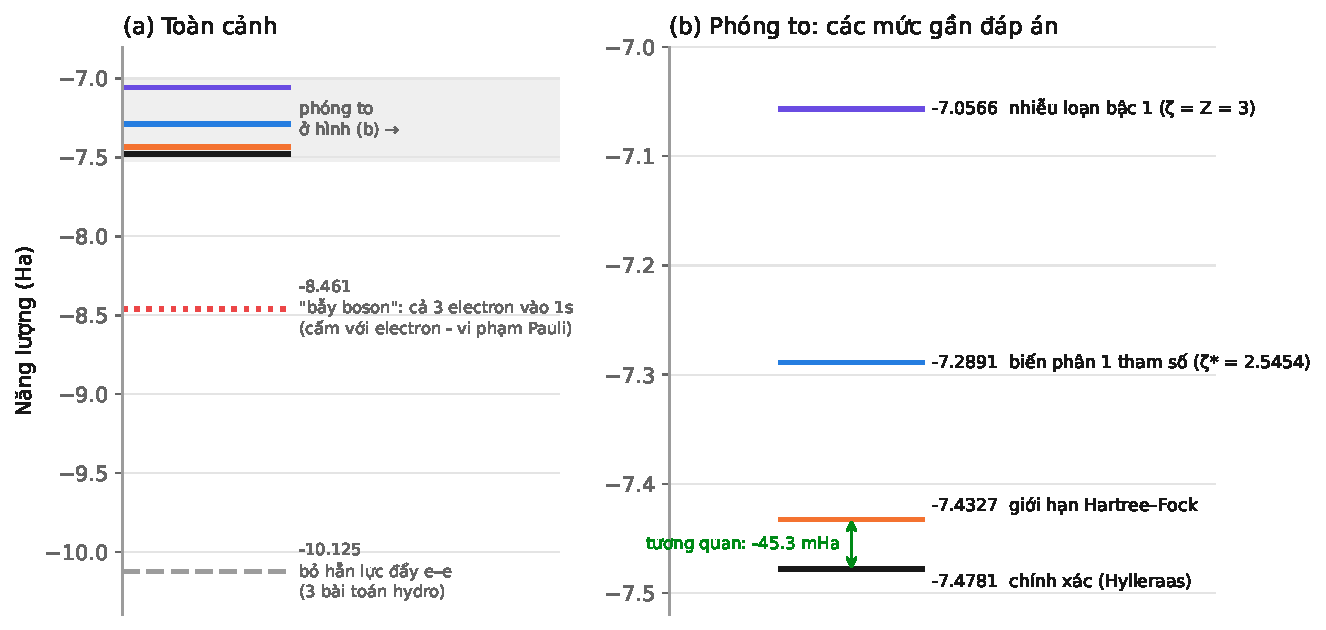
\includegraphics[width=\textwidth]{01_bac_thang_li.pdf}
\caption{Các mức xấp xỉ năng lượng của Li. Bỏ lực đẩy cho $-10.125\Ha$ (không phải biến phân vì đã đổi Hamiltonian). Hàm một tham số cho $-7.289\Ha$, giới hạn Hartree--Fock là $-7.433\Ha$, đáp án là $-7.478\Ha$. Vạch đỏ chấm là ``bẫy boson'': nếu quên tính phản đối xứng và cho cả 3 electron vào 1s, năng lượng xuống tới $-8.461\Ha$, \emph{thấp hơn} đáp án thật. (Script \code{01\_nen\_tang.py})}
\label{fig:bacthang}
\end{figure}

\begin{hieulam}[cái bẫy boson]
Hàm thử cho cả 3 electron vào 1s cho $E=-8.461\Ha$, thấp hơn năng lượng thật của Li. Có mâu thuẫn với nguyên lý biến phân không? Không: nguyên lý chỉ đảm bảo cận trên cho trạng thái thấp nhất \emph{trong lớp đối xứng mà hàm thử thuộc về}. Hàm không phản đối xứng thuộc ``thế giới boson'', nơi trạng thái thấp nhất nằm dưới trạng thái thấp nhất của fermion. Bài học: hàm thử \emph{bắt buộc} phải đúng đối xứng.
\end{hieulam}

\section{Năng lượng tương quan}\label{sec:tuongquan}

\begin{eli5}[quảng trường đông người]
Phương pháp Hartree--Fock (chương~\ref{ch:hf}) là hàm sóng dạng \emph{một} định thức Slater tốt nhất có thể. Nó giống như mỗi người trong một quảng trường đông đúc chỉ phản ứng với ``độ đông trung bình'' của đám đông, không nhìn từng người cụ thể. Ngoài đời, mọi người \emph{né nhau} từng bước một. Phần năng lượng mà cách nhìn ``trung bình'' bỏ sót gọi là \textbf{năng lượng tương quan}.

Quanh mỗi electron có hai ``bong bóng riêng tư''. \textbf{Lỗ Fermi} đẩy các electron \emph{cùng spin} ra xa; nó do Pauli gây ra và Hartree--Fock đã mô tả đúng. \textbf{Lỗ Coulomb} là phần né nhau thêm do lực đẩy tĩnh điện, nhất là giữa các electron \emph{ngược spin}; Hartree--Fock bỏ sót phần này.
\end{eli5}

\begin{congthuc}[định nghĩa của Löwdin]
\[
\Ecorr = E_{\text{chính xác}} - \EHF \;<\; 0 .
\]
$\EHF$ là năng lượng Hartree--Fock ở giới hạn tập cơ sở vô hạn. $\Ecorr$ luôn âm vì Hartree--Fock là phương pháp biến phân \cite{Lowdin1955}. Với Li:
\[
\Ecorr(\text{Li})=-7.478\,060-(-7.432\,727)=-0.045\,333\Ha=-1.234\eV .
\]
\end{congthuc}

Năng lượng tương quan chỉ chiếm 0.6\% tổng năng lượng của Li. Có nên bỏ qua không? Không, vì nó cỡ $28$\,kcal/mol, gấp 28 lần ``độ chính xác hóa học'' $1$\,kcal/mol ($1.6\mHa$). Đó là mức chính xác cần để dự đoán đúng một phản ứng hóa học có xảy ra hay không. Năng lượng liên kết hóa học cũng chỉ cỡ vài eV. Tính sai $\Ecorr$ là tính sai hóa học.

\begin{table}[h]
\centering\small
\caption{Năng lượng tương quan của vài nguyên tử và ion nhẹ \cite{King2018,KogaThakkar1996,Wang2012,Hornyak2019}.}
\label{tab:ecorr}
\begin{tabular}{@{}lrrrr@{}}
\toprule
Hệ & $\Ecorr$ (Ha) & $\Ecorr$ (eV) & kcal/mol & \% của $|E|$ \\
\midrule
He & $-0.042\,044$ & $-1.144$ & $-26.4$ & 1.45 \\
Li$^+$ (1s$^2$) & $-0.043\,498$ & $-1.184$ & $-27.3$ & 0.60 \\
Li (1s$^2$2s) & $-0.045\,333$ & $-1.234$ & $-28.4$ & 0.61 \\
Be (1s$^2$2s$^2$) & $-0.094\,333$ & $-2.567$ & $-59.2$ & 0.64 \\
\bottomrule
\end{tabular}
\end{table}

Một nhận xét thú vị từ bảng~\ref{tab:ecorr}: $\Ecorr(\text{Li}^+)$ đã bằng khoảng 96\% $\Ecorr(\text{Li})$. Tức là phần lớn tương quan của Li nằm ở \textbf{cặp electron lõi 1s$^2$}, hai electron ngược spin bị nén sát nhau quanh hạt nhân. Electron 2s ở xa nên chỉ đóng góp thêm khoảng $-1.8\mHa$. Chương~\ref{ch:sauhf} sẽ cho thấy hệ quả thực tế: tập cơ sở phải có đủ hàm để mô tả tương quan ở lõi.

\subsection{Tương quan động và tương quan tĩnh}
Người ta chia tương quan làm hai loại \cite{HollettGill2011}. \textbf{Tương quan động} \en{dynamic correlation} là việc electron né nhau ở khoảng cách ngắn, khắp mọi nơi và mọi lúc. \textbf{Tương quan tĩnh} \en{static correlation} xuất hiện khi có vài cấu hình electron gần như cùng năng lượng, nên một định thức duy nhất là không đủ. Be là ví dụ kinh điển: cấu hình 1s$^2$2p$^2$ trộn mạnh với 1s$^2$2s$^2$. Li chỉ có một electron hóa trị nên tương quan gần như hoàn toàn là \emph{động}. Đó là một lý do Li là ví dụ ``sạch'' để học.

\subsection{Điều kiện ``mũi nhọn'' của Kato}\label{sec:cusp}
Khi hai hạt tích điện tiến sát nhau ($r\to0$), thế Coulomb $\pm1/r$ tiến ra vô cùng. Để tổng $\Hhat\Psi$ vẫn hữu hạn, động năng phải ``bù'' lại vô cùng đó, và điều này buộc hàm sóng có một điểm gãy nhọn như đỉnh lều. Kato chứng minh điều này năm 1957 \cite{Kato1957}:

\begin{congthuc}[điều kiện cusp]
\begin{itemize}
\item Electron--hạt nhân: $\dfrac{\partial\bar\Psi}{\partial r_i}\Big|_{r_i=0}=-Z\,\Psi\big|_{r_i=0}$. Với hydro $\psi=e^{-Zr}$, ta có đúng $\psi'(0)=-Z\psi(0)$.
\item Hai electron ngược spin: $\dfrac{\partial\bar\Psi}{\partial r_{ij}}\Big|_{r_{ij}=0}=+\tfrac12\,\Psi\big|_{r_{ij}=0}$, tức gần điểm va chạm $\Psi\approx\Psi(0)(1+\tfrac12r_{ij})$.
\item Hai electron cùng spin: $\Psi=0$ tại điểm va chạm (lỗ Fermi), và hệ số tương ứng là $\tfrac14$.
\end{itemize}
($\bar\Psi$ là trung bình trên mặt cầu nhỏ quanh điểm va chạm.)
\end{congthuc}

Điều kiện cusp electron--electron giải thích vì sao các phương pháp dựng hàm sóng từ orbital (CI, Coupled Cluster) hội tụ \emph{chậm}: tổ hợp của các hàm mượt rất khó tạo ra một điểm gãy nhọn theo $r_{12}$. Với He, dù dùng orbital tới mômen động lượng $l=15$, CI vẫn sai $4.3$\,µHa \cite{Ruiz2021}. Lời giải, từ Hylleraas năm 1929, là đưa thẳng $r_{12}$ vào hàm sóng. Đó là bí quyết của các con số 15 chữ số ở bảng~\ref{tab:chuso}, và cũng là ý tưởng của thừa số Jastrow trong Monte Carlo lượng tử (chương~\ref{ch:qmc}).

\section{Bảng giá trị tham chiếu cho Li}

\begin{table}[h]
\centering\small
\caption{Các giá trị tham chiếu dùng xuyên suốt tài liệu (phi tương đối tính, hạt nhân cố định, trừ năng lượng ion hóa thực nghiệm).}
\label{tab:thamchieu}
\begin{tabularx}{\textwidth}{@{}Xrl@{}}
\toprule
Đại lượng & Giá trị & Nguồn \\
\midrule
Năng lượng chính xác $E(\text{Li})$ & $-7.478\,060\,323\,910\Ha$ & \cite{Wang2012,PKP2009} \\
Giới hạn Hartree--Fock $\EHF(\text{Li})$ (ROHF) & $-7.432\,726\,931\Ha$ & \cite{KogaThakkar1996} \\
Năng lượng tương quan $\Ecorr(\text{Li})$ & $-0.045\,333\Ha$ & tính từ hai dòng trên \\
$E(\text{Li}^+)$, cấu hình 1s$^2$ & $-7.279\,913\,412\,669\Ha$ & \cite{Nakashima2007} \\
$E(\text{Li}^{2+})$, cấu hình 1s & $-4.5\Ha$ (chính xác) & lời giải hydro \\
Năng lượng ion hóa thứ nhất, thực nghiệm & $5.391\,715\eV$ & \cite{NIST-ASD} \\
Năng lượng ion hóa thứ nhất, từ $E(\text{Li}^+)-E(\text{Li})$ & $5.391\,85\eV$ & tính toán \\
\bottomrule
\end{tabularx}
\end{table}

\begin{ghinho}
\begin{itemize}
\item Electron là fermion: hàm sóng đổi dấu khi đổi chỗ hai electron. Định thức Slater tự động thỏa điều này, và nguyên lý Pauli là hệ quả trực tiếp.
\item Nguyên lý biến phân: năng lượng của mọi hàm thử (đúng đối xứng) đều $\ge E_0$. Sai số năng lượng là bậc hai theo sai số hàm sóng.
\item Năng lượng tương quan $\Ecorr=E_{\text{chính xác}}-\EHF$. Với Li là $-45.3\mHa$, chỉ 0.6\% tổng năng lượng nhưng gấp 28 lần độ chính xác hóa học. Phần lớn nằm ở cặp lõi 1s$^2$.
\item Hàm sóng chính xác có ``mũi nhọn'' (cusp) khi hai hạt va chạm. Hàm dựng từ orbital mượt khó tạo ra mũi nhọn này, nên hội tụ chậm.
\end{itemize}
\end{ghinho}

\chapter{Hartree--Fock: ý tưởng trường trung bình}
\label{ch:hf}

\section{Ý tưởng: thay ``đám đông thật'' bằng ``đám đông trung bình''}

\begin{eli5}[sàn nhảy đông người]
Bạn nhảy trên một sàn nhảy đông người. Liên tục né từng người cụ thể thì quá phức tạp, nên bạn chỉ cảm nhận ``mật độ đám đông trung bình'': chỗ nào thường đông thì tránh, chỗ nào thưa thì tới. Mọi người khác cũng làm y như vậy. Nhưng ``đám đông trung bình'' lại do chính mọi người tạo ra, nên cả nhóm phải điều chỉnh qua lại cho tới khi bức tranh ổn định: không ai muốn đổi chỗ nữa. Đó là ý tưởng \textbf{trường trung bình} \en{mean field} và \textbf{trường tự hợp} \en{self-consistent field, SCF}.

\emph{Chỗ ví dụ ``gãy'':} người thật né nhau \emph{tức thời} (thấy người kia lao tới thì tránh). Mô hình trung bình bỏ mất điều đó, và phần bị bỏ mất chính là năng lượng tương quan.
\end{eli5}

Ý tưởng này biến bài toán $N$ electron dính chùm thành $N$ bài toán một electron, mỗi bài toán là một electron chuyển động trong ``trường'' của hạt nhân cộng với đám mây trung bình của các electron còn lại. Bài toán một electron thì ta giải được.

\subsection{Phương pháp Hartree (1928)}
Năm 1928, Douglas Hartree giả thiết hàm sóng là tích Hartree $\Psi=\phi_1(\vr_1)\phi_2(\vr_2)\phi_3(\vr_3)$, và mỗi orbital thỏa \cite{Hartree1928a}
\[
\Big[-\tfrac12\nabla^2-\frac{Z}{r}+\sum_{j\neq i}\int\frac{|\phi_j(\vr')|^2}{|\vr-\vr'|}\,d\vr'\Big]\phi_i(\vr)=\varepsilon_i\,\phi_i(\vr).
\]
Số hạng tích phân là thế tĩnh điện do ``đám mây điện tích'' $|\phi_j|^2$ của các electron \emph{khác} tạo ra. Vì thế này phụ thuộc vào chính các orbital cần tìm, ta phải lặp: đoán orbital, tính thế, giải phương trình được orbital mới, rồi lặp lại cho tới khi ``trường vào bằng trường ra''. Hartree gọi đó là \emph{self-consistent field}.

Thiếu sót của Hartree: tích Hartree không phản đối xứng (chương~\ref{ch:hatdongnhat}). Năm 1930, Fock và Slater độc lập sửa lỗi này bằng cách thay tích Hartree bằng định thức Slater \cite{Fock1930,Slater1930}. Kết quả là phương pháp \textbf{Hartree--Fock} (HF). Li là một trong những nguyên tử đầu tiên được tính bằng HF đầy đủ: Fock và Petrashen, năm 1935.

\section{Phương trình Hartree--Fock}

Phương pháp HF tìm \emph{định thức Slater tốt nhất}: chọn các orbital sao cho năng lượng $E=\langle\Psi_0|\Hhat|\Psi_0\rangle$ nhỏ nhất. Theo nguyên lý biến phân, $\EHF\ge E_{\text{chính xác}}$.

\begin{congthuc}[năng lượng HF của Li]
Với định thức $|1s\!\uparrow\,1s\!\downarrow\,2s\!\uparrow|$ (orbital 1s dùng chung cho hai spin, gọi là ROHF), áp dụng quy tắc Slater--Condon \cite{Szabo1996}:
\[
E_{\rm HF}(\text{Li})=2h_{1s}+h_{2s}+J_{1s1s}+2J_{1s2s}-K_{1s2s}.
\]
\begin{itemize}
\item $h_{a}=\int\phi_a^*(\vr)\big[-\tfrac12\nabla^2-\tfrac{Z}{r}\big]\phi_a(\vr)\,d\vr$: động năng cộng hút hạt nhân của một electron ở orbital $a$.
\item $J_{ab}=\iint\dfrac{|\phi_a(\vr_1)|^2\,|\phi_b(\vr_2)|^2}{r_{12}}\,d\vr_1d\vr_2$: \textbf{tích phân Coulomb}, lực đẩy tĩnh điện giữa hai đám mây điện tích $|\phi_a|^2$ và $|\phi_b|^2$. Có ý nghĩa cổ điển rõ ràng.
\item $K_{ab}=\iint\dfrac{\phi_a^*(\vr_1)\phi_b(\vr_1)\,\phi_b^*(\vr_2)\phi_a(\vr_2)}{r_{12}}\,d\vr_1d\vr_2$: \textbf{tích phân trao đổi}. Chỉ xuất hiện giữa hai electron \emph{cùng spin}. Không có tương tự cổ điển: nó là hệ quả của tính phản đối xứng.
\end{itemize}
Với Li: $J_{1s1s}$ là đẩy giữa hai electron 1s (khác spin, nên không có $K$); $2J_{1s2s}$ là electron 2s đẩy cả hai electron 1s; $-K_{1s2s}$ chỉ có một lần, cho cặp cùng spin 1s$\uparrow$--2s$\uparrow$.
\end{congthuc}

\begin{congthuc}[toán tử Fock]
Cực tiểu hóa năng lượng (với ràng buộc các orbital trực chuẩn) dẫn tới phương trình trị riêng cho từng spin-orbital:
\[
\hat f\,\chi_a=\varepsilon_a\,\chi_a,\qquad \hat f=\underbrace{-\tfrac12\nabla^2-\frac{Z}{r}}_{\hat h}+\sum_{b}\big[\hat J_b-\hat K_b\big].
\]
\begin{itemize}
\item $\hat J_b\chi_a(\vr_1)=\Big[\int\frac{|\chi_b(\vx_2)|^2}{r_{12}}d\vx_2\Big]\chi_a(\vr_1)$: nhân với thế tĩnh điện của electron $b$. Toán tử \emph{cục bộ}: giá trị tại $\vr_1$ chỉ cần biết $\chi_a$ tại $\vr_1$.
\item $\hat K_b\chi_a(\vr_1)=\Big[\int\frac{\chi_b^*(\vx_2)\chi_a(\vx_2)}{r_{12}}d\vx_2\Big]\chi_b(\vr_1)$: ``tráo'' nhãn $a\leftrightarrow b$. Toán tử \emph{phi cục bộ}: cần biết $\chi_a$ trên toàn không gian.
\item $\varepsilon_a$: \textbf{năng lượng orbital}.
\end{itemize}
Vì $\hat J_a\chi_a=\hat K_a\chi_a$, số hạng $b=a$ tự triệt tiêu: \textbf{electron không tự đẩy chính mình}. Đây là một ưu điểm của HF mà ta sẽ nhắc lại khi nói về lỗi ``tự tương tác'' của DFT (chương~\ref{ch:dft}).
\end{congthuc}

\begin{eli5}[trao đổi]
Hai electron cùng spin giống hai cầu thủ cùng áo bị luật chơi cấm đứng chung một chỗ. Không ai đẩy ai, nhưng quanh mỗi người vẫn có một ``vùng cấm'' với đồng đội (lỗ Fermi). Vì tự động đứng xa nhau hơn, lực đẩy trung bình giữa họ nhỏ đi, nên năng lượng giảm một lượng $K$. Hai electron \emph{khác} spin không bị luật này ràng buộc. Trong HF, chúng hoàn toàn ``không biết'' vị trí tức thời của nhau.
\end{eli5}

Điều cuối cùng là chìa khóa: \emph{trong HF, electron cùng spin đã ``né'' nhau (nhờ phản đối xứng), còn electron khác spin thì không} \cite{Szabo1996}. Với Li, hai electron 1s có spin ngược nhau và ở rất gần nhau. HF bỏ qua hoàn toàn việc chúng né nhau, và đó là nguồn của phần lớn năng lượng tương quan của Li.

\section{Vòng lặp trường tự hợp}

Toán tử Fock phụ thuộc vào chính các orbital ($\hat J_b,\hat K_b$ được tính từ $\chi_b$), nên phương trình HF là phi tuyến. Cách giải: lặp.

\begin{congthuc}[thuật toán SCF dạng ma trận]
Biểu diễn mỗi orbital bằng tổ hợp tuyến tính của $K$ hàm cơ sở $\{g_\mu\}$ đã biết (mục~\ref{sec:tapcoso}): $\phi_i=\sum_\mu C_{\mu i}\,g_\mu$. Bài toán vi phân trở thành bài toán ma trận \textbf{Roothaan--Hall} \cite{Roothaan1951}:
\[
\mathbf F\,\mathbf C=\mathbf S\,\mathbf C\,\boldsymbol\varepsilon .
\]
\begin{enumerate}
\item Tính trước các tích phân: ma trận chồng phủ $S_{\mu\nu}=\int g_\mu g_\nu$; Hamiltonian lõi $H_{\mu\nu}=\int g_\mu\hat h\, g_\nu$; tích phân đẩy $(\mu\nu|\lambda\sigma)=\iint g_\mu(1)g_\nu(1)\frac{1}{r_{12}}g_\lambda(2)g_\sigma(2)$.
\item Đoán ma trận mật độ ban đầu $\mathbf D$ (ví dụ: bỏ qua lực đẩy, chỉ chéo hóa $\mathbf H$).
\item Dựng ma trận Fock cho từng spin: $\mathbf F^\alpha=\mathbf H+\mathbf J[\mathbf D^\alpha+\mathbf D^\beta]-\mathbf K[\mathbf D^\alpha]$, với $J_{\mu\nu}=\sum_{\lambda\sigma}(\mu\nu|\lambda\sigma)D_{\lambda\sigma}$ và $K_{\mu\nu}=\sum_{\lambda\sigma}(\mu\lambda|\nu\sigma)D_{\lambda\sigma}$.
\item Giải bài toán trị riêng $\mathbf F\mathbf C=\mathbf S\mathbf C\boldsymbol\varepsilon$, được orbital mới $\mathbf C$.
\item Mật độ mới: $D^\alpha_{\mu\nu}=\sum_{i\in\text{chiếm}}C_{\mu i}C_{\nu i}$ (tổng trên $N_\alpha$ orbital thấp nhất).
\item Nếu năng lượng và mật độ thay đổi đủ nhỏ thì dừng; nếu không, quay lại bước 3.
\end{enumerate}
Năng lượng ở mỗi vòng: $E=\tfrac12\sum_{\mu\nu}\big[(D^\alpha+D^\beta)_{\mu\nu}H_{\mu\nu}+D^\alpha_{\mu\nu}F^\alpha_{\mu\nu}+D^\beta_{\mu\nu}F^\beta_{\mu\nu}\big]$.
\end{congthuc}

\begin{chaycode}[tự viết Hartree--Fock trong 30 dòng]
Hàm \code{my\_uhf} trong \code{code/02\_hartree\_fock.py} cài đặt đúng thuật toán trên chỉ bằng \code{numpy}. PySCF chỉ dùng để tính các tích phân đầu vào. Lõi của vòng lặp:
\begin{verbatim}
for it in range(1, max_iter + 1):
    J  = einsum("pqrs,rs->pq", eri, Da + Db)   # Coulomb
    Ka = einsum("prqs,rs->pq", eri, Da)        # trao đổi, spin lên
    Kb = einsum("prqs,rs->pq", eri, Db)        # trao đổi, spin xuống
    Fa, Fb = H + J - Ka, H + J - Kb            # hai ma trận Fock
    E  = 0.5 * sum((Da + Db) * H + Da * Fa + Db * Fb)
    ea, Ca = solve(Fa);  eb, Cb = solve(Fb)    # FC = SCe
    Da = Ca[:, :2] @ Ca[:, :2].T               # 2 electron spin lên
    Db = Cb[:, :1] @ Cb[:, :1].T               # 1 electron spin xuống
\end{verbatim}
Với tập cơ sở cc-pCVTZ (43 hàm), vòng lặp hội tụ sau 26 vòng về $E=-7.432\,702\,938\Ha$, trùng với PySCF tới $4\times10^{-14}\Ha$.
\end{chaycode}

\begin{figure}[h]
\centering
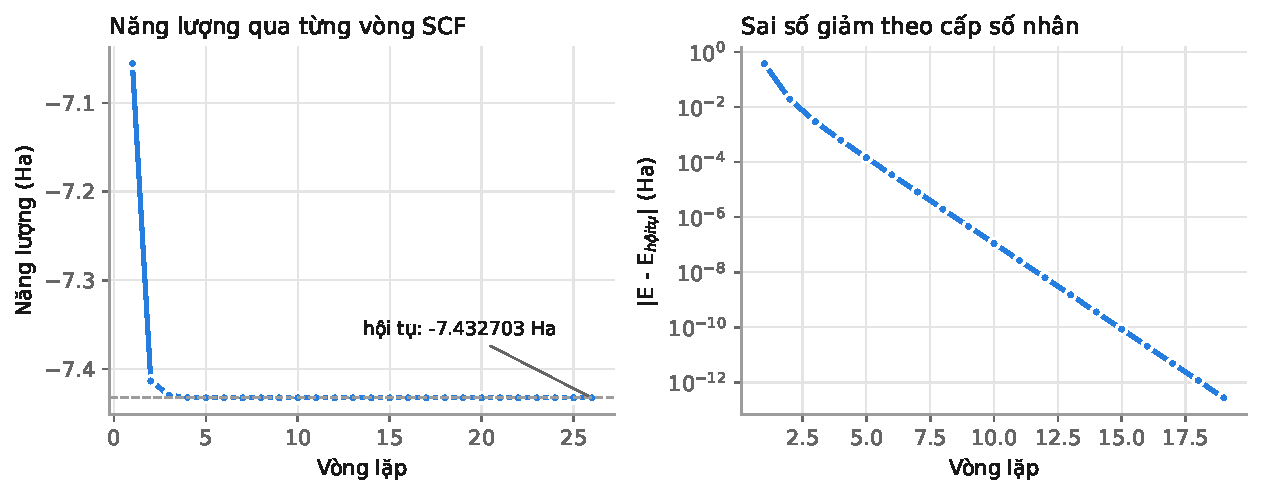
\includegraphics[width=\textwidth]{02_scf_hoi_tu.pdf}
\caption{Vòng lặp SCF tự viết cho Li (UHF/cc-pCVTZ). Trái: năng lượng giảm từ $-7.056\Ha$ (vòng 1) và ổn định gần như ngay lập tức. Phải: sai số so với giá trị hội tụ giảm theo cấp số nhân, mỗi vòng khoảng 3--4 lần, cho tới giới hạn làm tròn của máy tính. (Script \code{02\_hartree\_fock.py})}
\label{fig:scf}
\end{figure}

\begin{hieulam}[``tự hợp'' nghĩa là ``đúng'']
Tự hợp chỉ có nghĩa là lời giải tạo ra đúng cái trường mà nó đã giả định. Lời giải tự hợp của HF vẫn thiếu năng lượng tương quan. Ngoài ra vòng lặp có thể dao động hoặc rơi vào một nghiệm không phải thấp nhất. Các chương trình thực tế dùng kỹ thuật tăng tốc như DIIS \cite{Pulay1980} để hội tụ nhanh và ổn định hơn.
\end{hieulam}

\section{Tập cơ sở: xếp Lego để vẽ orbital}\label{sec:tapcoso}

\begin{eli5}[Lego]
Thay vì vẽ hình dạng orbital tự do (cần vô số điểm), ta ``xếp Lego'': orbital là tổng của một số khối có hình dạng cố định, nhân với các hệ số điều chỉnh được. Bộ khối đó gọi là \textbf{tập cơ sở} \en{basis set}. Càng nhiều khối và khối càng đa dạng, hình vẽ càng sát thật. Bài toán vi phân trở thành bài toán ma trận, loại bài toán máy tính giải rất giỏi.
\end{eli5}

\paragraph{Hàm Slater và hàm Gauss.}
Lựa chọn tự nhiên là \textbf{hàm kiểu Slater} (STO) $r^{n-1}e^{-\zeta r}Y_{lm}$, có đúng mũi nhọn ở hạt nhân và đuôi suy giảm như nghiệm thật. Nhưng tích phân bốn tâm của STO rất khó tính. Năm 1950, Boys đề xuất dùng \textbf{hàm kiểu Gauss} (GTO) $x^ay^bz^c\,e^{-\alpha r^2}$ \cite{Boys1950}. Hàm Gauss có hình dạng ``sai'' (đỉnh tròn thay vì nhọn, đuôi tắt quá nhanh), nhưng có một tính chất thần kỳ:
\[
e^{-\alpha|\vr-\mathbf A|^2}\,e^{-\beta|\vr-\mathbf B|^2}=e^{-\frac{\alpha\beta}{\alpha+\beta}|\mathbf A-\mathbf B|^2}\;e^{-(\alpha+\beta)|\vr-\mathbf P|^2},\quad \mathbf P=\frac{\alpha\mathbf A+\beta\mathbf B}{\alpha+\beta}.
\]
Tích của hai hàm Gauss đặt ở hai tâm là một hàm Gauss đặt ở tâm thứ ba. Nhờ vậy mọi tích phân đều tính được bằng công thức, rất nhanh. Dùng nhiều hàm Gauss vẫn rẻ hơn dùng ít hàm Slater. Gần như mọi chương trình hóa lượng tử hiện nay dùng hàm Gauss.

\paragraph{Các họ tập cơ sở.}
\begin{itemize}
\item \textbf{STO-3G} \cite{Hehre1969}: tập ``cực tiểu''. Mỗi orbital nguyên tử được xấp xỉ bằng 3 hàm Gauss. Li có 5 hàm (1s, 2s, 2p$_{x,y,z}$).
\item \textbf{6-31G}: lớp hóa trị được ``tách đôi'' để linh hoạt hơn. Li có 9 hàm.
\item \textbf{cc-pVXZ} (X = D, T, Q, 5 ứng với 2, 3, 4, 5) \cite{Dunning1989,Prascher2011}: họ ``tương quan nhất quán'' \en{correlation-consistent} của Dunning. Mỗi bậc X thêm một lớp hàm có mômen động lượng cao hơn. Li có 14, 30, 55, 91 hàm.
\item \textbf{cc-pCVXZ}: thêm các hàm ``chặt'' (tập trung gần hạt nhân) để mô tả tương quan của electron lõi. Li có 18, 43, 84 hàm. Chương~\ref{ch:sauhf} sẽ cho thấy với Li, loại này là \emph{bắt buộc}.
\end{itemize}

\begin{figure}[h]
\centering
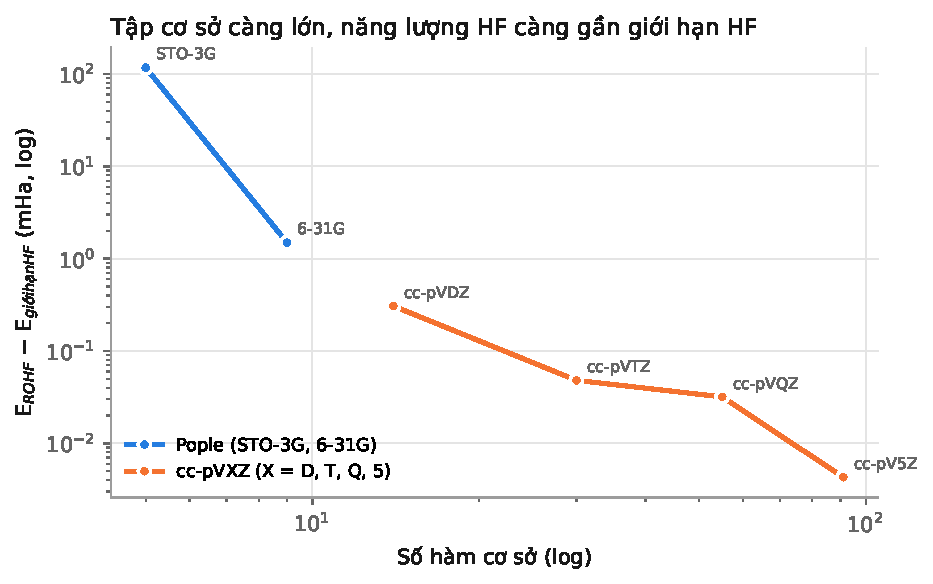
\includegraphics[width=0.82\textwidth]{02_hoi_tu_tap_co_so.pdf}
\caption{Năng lượng ROHF của Li hội tụ về giới hạn HF ($-7.432\,727\Ha$) khi tập cơ sở lớn dần. STO-3G sai $117\mHa$, cc-pV5Z chỉ còn sai $0.004\mHa$. (Script \code{02\_hartree\_fock.py})}
\label{fig:coso}
\end{figure}

\begin{table}[h]
\centering\small
\caption{Năng lượng ROHF của Li theo tập cơ sở (tính bằng code đi kèm). Các hàm lõi (cc-pCVXZ) hầu như không đổi năng lượng HF.}
\label{tab:hfcoso}
\begin{tabular}{@{}lrrr@{}}
\toprule
Tập cơ sở & Số hàm & $E_{\rm ROHF}$ (Ha) & Sai số so với giới hạn HF (mHa) \\
\midrule
STO-3G & 5 & $-7.315\,526$ & $117.20$ \\
6-31G & 9 & $-7.431\,235$ & $1.49$ \\
cc-pVDZ & 14 & $-7.432\,420$ & $0.307$ \\
cc-pVTZ & 30 & $-7.432\,679$ & $0.048$ \\
cc-pVQZ & 55 & $-7.432\,695$ & $0.032$ \\
cc-pV5Z & 91 & $-7.432\,723$ & $0.004$ \\
cc-pCVQZ & 84 & $-7.432\,695$ & $0.032$ \\
aug-cc-pCVQZ & 109 & $-7.432\,696$ & $0.031$ \\
\midrule
Giới hạn HF \cite{KogaThakkar1996} & $\infty$ & $-7.432\,727$ & 0 \\
\bottomrule
\end{tabular}
\end{table}

Năng lượng HF hội tụ rất nhanh theo tập cơ sở (gần như theo hàm mũ của X). Ta sẽ thấy ở chương sau rằng năng lượng tương quan hội tụ \emph{chậm hơn nhiều}, chỉ như $X^{-3}$, vì phải vẽ mũi nhọn electron--electron bằng các ``khối Lego'' tròn trịa.

\section{Vỏ mở: ROHF và UHF}

Li có một electron lẻ, nên có hai cách làm HF:
\begin{itemize}
\item \textbf{ROHF} \en{restricted open-shell}: hai electron 1s dùng \emph{chung} một orbital không gian. Hàm sóng có spin toàn phần đúng bằng $\tfrac12$.
\item \textbf{UHF} \en{unrestricted}: cho phép orbital của electron spin lên và spin xuống khác nhau. Năng lượng thấp hơn (vì linh hoạt hơn), nhưng hàm sóng không còn là trạng thái spin ``sạch''.
\end{itemize}

Trong UHF, electron 2s$\uparrow$ có tương tác trao đổi với 1s$\uparrow$ nhưng không với 1s$\downarrow$, nên hai orbital 1s tách nhau một chút. Năng lượng orbital tính được: $\varepsilon_{1s\uparrow}=-2.4867\Ha$ và $\varepsilon_{1s\downarrow}=-2.4687\Ha$. Hiện tượng này gọi là \textbf{phân cực spin lõi}. Nó có thật: nó làm mật độ spin tại hạt nhân khác 0 và ảnh hưởng tới phổ siêu tinh tế đo được của Li \cite{Sachs1960}.

\begin{congthuc}[nhiễm bẩn spin]
Với trạng thái doublet thuần, $\langle\hat S^2\rangle=S(S+1)=0.75$. Hàm UHF có thể lẫn một chút trạng thái quartet ($S=\tfrac32$), làm $\langle\hat S^2\rangle>0.75$. Với Li/aug-cc-pCVQZ, code cho:
\[
E_{\rm ROHF}=-7.432\,696\Ha,\quad E_{\rm UHF}=-7.432\,720\Ha,\quad \langle\hat S^2\rangle_{\rm UHF}=0.750\,016 .
\]
Nhiễm bẩn rất nhỏ, và UHF chỉ thấp hơn ROHF $0.024\mHa$. Với Li, chọn cách nào cũng được. Với các hệ khác (phân tử bị kéo giãn, gốc tự do) nhiễm bẩn spin có thể lớn và gây sai lệch nghiêm trọng.
\end{congthuc}

\section{Định lý Koopmans: năng lượng orbital có nghĩa gì?}

\begin{eli5}[chụp ảnh tập thể]
Bạn muốn ước tính ``giá'' của việc rút một người ra khỏi bức ảnh tập thể. Cách nhanh nhất: giả sử những người còn lại đứng yên không nhúc nhích. Đó là ý tưởng của định lý Koopmans. Ngoài đời, khi một người rời đi, những người còn lại sẽ xê dịch (gọi là \emph{hồi phục orbital}), và cách họ né nhau cũng thay đổi (tương quan).
\end{eli5}

\begin{congthuc}[định lý Koopmans]
Nếu các orbital còn lại ``đông cứng'' khi lấy electron khỏi orbital $a$, năng lượng ion hóa bằng trừ năng lượng orbital \cite{Koopmans1934}:
\[
\text{IE}_a\approx-\varepsilon_a .
\]
\end{congthuc}

\begin{table}[h]
\centering\small
\caption{Năng lượng ion hóa thứ nhất của Li (tính bằng code, tập cơ sở aug-cc-pCVQZ).}
\label{tab:koopmans}
\begin{tabular}{@{}lrr@{}}
\toprule
Cách tính & IE (eV) & Sai số (eV) \\
\midrule
Koopmans: $-\varepsilon_{2s}$ (UHF) & 5.343 & $-0.049$ \\
$\Delta$SCF: $E_{\rm HF}(\text{Li}^+)-E_{\rm HF}(\text{Li})$ & 5.343 & $-0.049$ \\
Từ năng lượng chính xác: $E(\text{Li}^+)-E(\text{Li})$ & 5.392 & $+0.000$ \\
Thực nghiệm \cite{NIST-ASD} & 5.392 & --- \\
\bottomrule
\end{tabular}
\end{table}

Bảng~\ref{tab:koopmans} kể một câu chuyện thú vị. Koopmans và $\Delta$SCF gần như trùng nhau, nghĩa là hiệu ứng hồi phục orbital rất nhỏ: rút electron 2s ở xa ra hầu như không làm lõi 1s$^2$ co lại. Cả hai đều thiếu đúng $0.050\eV$. Con số này chính là \emph{hiệu năng lượng tương quan} giữa Li và Li$^+$: $\Ecorr(\text{Li})-\Ecorr(\text{Li}^+)=-45.33-(-43.50)=-1.83\mHa=-0.050\eV$. Khi dùng năng lượng chính xác, sai số biến mất. Năm 1936, James và Coolidge đã nhận ra đúng sai số $0.05\eV$ này khi dùng hàm sóng không tính tới chuyển động tương đối giữa electron lớp K và lớp L \cite{JamesCoolidge1936}.

\section{Hartree--Fock bỏ sót gì?}
HF cho Li năng lượng $-7.432\,727\Ha$, đúng 99.4\% năng lượng toàn phần. Nhưng như đã nói ở chương~\ref{ch:hatdongnhat}, phần 0.6\% còn thiếu ($45.3\mHa$) gấp 28 lần độ chính xác hóa học. Phần thiếu đến từ việc các electron \emph{khác spin} chuyển động hoàn toàn độc lập trong HF: hai electron 1s có thể ``đứng'' cùng một chỗ với xác suất bằng tích xác suất riêng lẻ, trong khi thực tế chúng né nhau. Chương tiếp theo trình bày các cách sửa lỗi này một cách có hệ thống.

\begin{ghinho}
\begin{itemize}
\item HF tìm định thức Slater tốt nhất. Mỗi electron chuyển động trong trường trung bình của hạt nhân và các electron khác. Phương trình phi tuyến nên phải lặp tới tự hợp (SCF).
\item Năng lượng gồm phần Coulomb $J$ (cổ điển) và phần trao đổi $-K$ (chỉ giữa electron cùng spin, thuần lượng tử). HF không có lỗi tự tương tác.
\item Orbital được biểu diễn bằng tập cơ sở Gauss; phương trình thành bài toán ma trận $\mathbf{FC}=\mathbf{SC}\boldsymbol\varepsilon$. HF hội tụ nhanh theo tập cơ sở.
\item Với Li: $\EHF=-7.432\,727\Ha$; Koopmans cho IE $=5.34\eV$ (thực nghiệm 5.39). Phần thiếu là tương quan, chủ yếu giữa hai electron 1s khác spin.
\end{itemize}
\end{ghinho}

\chapter{Sau Hartree--Fock: CI, MP2 và Coupled Cluster}
\label{ch:sauhf}

Hartree--Fock cho ta một định thức Slater tốt nhất. Các phương pháp ``sau Hartree--Fock'' \en{post-Hartree--Fock} đi tiếp từ đó và cố gắng thu lại năng lượng tương quan còn thiếu. Chương này trình bày ba ý tưởng chính: trộn thêm nhiều định thức (CI), coi tương quan như một nhiễu loạn nhỏ (MP2), và ``lãi kép'' các kích thích (Coupled Cluster).

\section{Tương tác cấu hình (CI): pha màu}

\begin{eli5}[pha màu]
Màu thật (hàm sóng đúng) được pha từ một màu nền (định thức HF) với một chút các màu khác. Mỗi ``màu khác'' là một \textbf{định thức kích thích} \en{excited determinant}: lấy 1, 2 hoặc 3 electron từ orbital đang có người lên các orbital còn trống (orbital ``ảo'' \en{virtual}). Dùng \emph{tất cả} các màu trong hộp gọi là \textbf{Full CI}: chính xác tuyệt đối \emph{với hộp màu đó} (tức là với tập cơ sở đã chọn). Hộp càng nhiều màu (tập cơ sở lớn) thì càng gần màu thật.

\emph{Chỗ ví dụ ``gãy'':} hệ số pha có thể âm (các định thức giao thoa triệt tiêu nhau), điều không xảy ra với sơn. Và số ``màu'' tăng nhanh khủng khiếp.
\end{eli5}

\begin{congthuc}[khai triển CI]
\[
|\Psi_{\rm CI}\rangle=c_0|\Phi_0\rangle+\sum_{a,r}c_a^r|\Phi_a^r\rangle+\sum_{\substack{a<b\\ r<s}}c_{ab}^{rs}|\Phi_{ab}^{rs}\rangle+\sum_{\substack{a<b<c\\ r<s<t}}c_{abc}^{rst}|\Phi_{abc}^{rst}\rangle+\cdots
\]
\begin{itemize}
\item $\Phi_0$: định thức HF. $\Phi_a^r$: định thức trong đó electron ở orbital chiếm $a$ được chuyển lên orbital ảo $r$ (kích thích đơn). $\Phi_{ab}^{rs}$: kích thích đôi, v.v.
\item Các hệ số $c$ tìm bằng cách chéo hóa ma trận $H_{IJ}=\langle\Phi_I|\Hhat|\Phi_J\rangle$. Trị riêng nhỏ nhất là năng lượng. Đây là phương pháp biến phân nên cho cận trên.
\item Cắt bớt theo bậc kích thích: CIS (đơn), CISD (đơn + đôi), CISDT\ldots{} Giữ tất cả là \textbf{Full CI} (FCI).
\item \textbf{Định lý Brillouin}: với định thức HF, $\langle\Phi_0|\Hhat|\Phi_a^r\rangle=0$. Kích thích đơn không trực tiếp hạ năng lượng; tương quan bắt đầu từ kích thích đôi, tức là \emph{từng cặp} electron cùng né nhau.
\end{itemize}
Với Li chỉ có 3 electron, bậc kích thích cao nhất là 3, nên CISDT đã là Full CI.
\end{congthuc}

\subsection{Bùng nổ tổ hợp}
Có bao nhiêu định thức? Với $M$ orbital không gian, $N_\alpha$ electron spin lên và $N_\beta$ electron spin xuống, số cách chọn là
\[
N_{\rm det}=\binom{M}{N_\alpha}\binom{M}{N_\beta}.
\]
Với Li ($N_\alpha=2,N_\beta=1$) trong tập cc-pCVQZ ($M=84$): $\binom{84}{2}\times84=3486\times84=292\,824$ định thức, một con số máy tính xách tay xử lý trong vài phút. Nhưng hình~\ref{fig:dinhthuc} cho thấy chuyện gì xảy ra khi số electron tăng: với Ne (10 electron) và 100 orbital đã có $\sim10^{15}$ định thức, còn với Fe là $\sim10^{31}$. Đây chính là bức tường hàm mũ của chương~\ref{ch:baitoan}, trong một bộ áo khác. Năm 2017, một nhóm nghiên cứu đã chạy được một vòng lặp CI với khoảng $10^{12}$ định thức trên siêu máy tính \cite{Vogiatzis2017}, cỡ giới hạn của công nghệ hiện nay.

\begin{figure}[h]
\centering
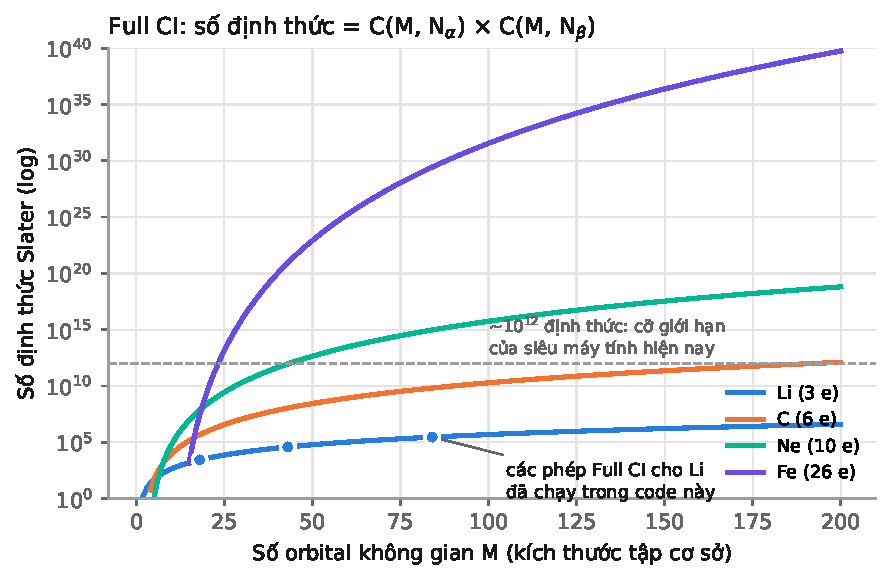
\includegraphics[width=0.84\textwidth]{03_bung_no_dinh_thuc.pdf}
\caption{Số định thức của Full CI theo số orbital, cho các nguyên tử có số electron khác nhau (trục tung thang log). Các chấm xanh là ba phép Full CI cho Li chạy trong code đi kèm. (Script \code{03\_sau\_hartree\_fock.py})}
\label{fig:dinhthuc}
\end{figure}

\subsection{Vấn đề ``nhất quán kích thước''}
CI cắt bớt (như CISD) có một khuyết tật tinh tế. Xét hai nguyên tử Li đặt cách nhau 50\,Å, xa tới mức không tương tác. Năng lượng của cặp phải đúng bằng hai lần năng lượng một nguyên tử. Nhưng hàm sóng đúng của cặp chứa số hạng ``kích thích đôi trên nguyên tử A \emph{nhân} kích thích đôi trên nguyên tử B'', tức là kích thích bậc 4 của cả hệ, mà CISD không có. Subagent nghiên cứu đã kiểm tra trực tiếp bằng PySCF (tập cc-pCVDZ): CISD cho năng lượng cặp cao hơn hai lần năng lượng một nguyên tử $0.19\mHa$, trong khi MP2 và CCSD cho đúng sai lệch bằng 0. Tính chất ``năng lượng của các mảnh không tương tác thì cộng được'' gọi là \textbf{nhất quán kích thước} \en{size-consistency}. Với hệ lớn, sai số của CISD tăng như $\sqrt{N}$ thay vì $N$, và tỉ lệ tương quan thu được trên mỗi phân tử tiến về 0 \cite{Szabo1996}. Đó là lý do CISD hầu như không còn được dùng.

\section{Lý thuyết nhiễu loạn Møller--Plesset (MP2)}

\begin{eli5}[giá khởi điểm và phụ phí]
Lấy năng lượng HF làm ``giá khởi điểm'', rồi cộng thêm một khoản ``phụ phí'' cho từng cặp electron, tính xem chúng muốn né nhau bao nhiêu. Phụ phí bậc 2 thường là phần lớn nhất. Nhanh, rẻ, nhưng nếu giá khởi điểm tệ (khi HF là bức tranh sai về chất) thì phụ phí có thể không còn ``nhỏ''.
\end{eli5}

\begin{congthuc}[MP2]
Coi Hamiltonian là tổng các toán tử Fock (bài toán đã giải được) cộng một nhiễu loạn $\hat V$. Bổ chính bậc 2 \cite{MollerPlesset1934}:
\[
E^{(2)}=\frac14\sum_{a,b}^{\text{chiếm}}\sum_{r,s}^{\text{ảo}}\frac{|\langle ab\|rs\rangle|^2}{\varepsilon_a+\varepsilon_b-\varepsilon_r-\varepsilon_s}\;<0 .
\]
\begin{itemize}
\item $\langle ab\|rs\rangle$: ``độ mạnh'' của việc đẩy cặp electron từ orbital $a,b$ lên $r,s$ (tích phân đẩy đã phản đối xứng hóa).
\item Mẫu số: chênh lệch năng lượng orbital, luôn âm. Kích thích càng ``đắt'' thì đóng góp càng nhỏ.
\end{itemize}
MP2 không cần lặp, chi phí tăng như $N^5$, nhất quán kích thước, nhưng \emph{không biến phân}: có thể cho năng lượng thấp hơn giá trị đúng.
\end{congthuc}

\section{Coupled Cluster: lãi kép thay vì lãi đơn}

\begin{eli5}[lãi kép]
CI cộng mỗi kích thích đúng một lần, giống ``lãi đơn''. Coupled Cluster đặt các kích thích vào \emph{số mũ}, giống ``lãi kép'': $e^{\hat T}=1+\hat T+\tfrac12\hat T^2+\tfrac16\hat T^3+\ldots$ Nhờ vậy nó tự động sinh ra mọi tổ hợp của các kích thích độc lập, ví dụ ``cặp này né nhau \emph{và đồng thời} cặp kia né nhau''. Hai phân tử ở xa nhau được mô tả đúng như hai hệ riêng biệt, tức là nhất quán kích thước.

\emph{Chỗ ví dụ ``gãy'':} CC không biến phân. Và nếu ``vốn ban đầu'' (định thức HF) sai về bản chất (khi cần nhiều định thức ngang nhau), thì lãi kép từ một số vốn sai vẫn sai.
\end{eli5}

\begin{congthuc}[Coupled Cluster]
\[
|\Psi_{\rm CC}\rangle=e^{\hat T}|\Phi_0\rangle,\qquad \hat T=\hat T_1+\hat T_2+\hat T_3+\ldots
\]
\begin{itemize}
\item $\hat T_1=\sum_{ar}t_a^r\,\hat a_r^\dagger\hat a_a$ tạo kích thích đơn với ``biên độ'' $t_a^r$; $\hat T_2=\tfrac14\sum t_{ab}^{rs}\hat a_r^\dagger\hat a_s^\dagger\hat a_b\hat a_a$ tạo kích thích đôi. ($\hat a^\dagger$, $\hat a$: toán tử ``đặt'' và ``nhấc'' một electron.)
\item Khai triển $e^{\hat T_2}=1+\hat T_2+\tfrac12\hat T_2^2+\ldots$: số hạng $\tfrac12\hat T_2^2$ là kích thích bậc 4 dạng ``đôi nhân đôi''. Đây đúng là thứ CISD thiếu.
\item Các biên độ $t$ được tìm bằng cách giải hệ phương trình phi tuyến (lặp). \textbf{CCSD} giữ $\hat T_1+\hat T_2$ \cite{PurvisBartlett1982}, chi phí $\sim N^6$.
\item \textbf{CCSD(T)} thêm ước lượng nhiễu loạn cho kích thích ba, chi phí $\sim N^7$ \cite{Raghavachari1989}. Đây được gọi là ``tiêu chuẩn vàng'' \en{gold standard} của hóa lượng tử cho các phân tử có một cấu hình chiếm ưu thế \cite{BartlettMusial2007}.
\end{itemize}
\end{congthuc}

\begin{table}[h]
\centering\small
\caption{Thứ bậc các phương pháp hàm sóng. $N$ là kích thước hệ (số electron hoặc số hàm cơ sở) \cite{BartlettMusial2007,Szabo1996}.}
\label{tab:chiphi}
\begin{tabular}{@{}llccl@{}}
\toprule
Phương pháp & Chi phí & Biến phân? & Nhất quán kích thước? & Ghi chú \\
\midrule
HF & $N^4$ & có & có & không có tương quan \\
MP2 & $N^5$ & không & có & rẻ, thường thu 80--95\% tương quan \\
CISD & $N^6$ & có & \textbf{không} & ít dùng vì lỗi kích thước \\
CCSD & $N^6$ & không & có & lặp \\
CCSD(T) & $N^7$ & không & có & ``tiêu chuẩn vàng'' \\
Full CI & tổ hợp ($\sim e^N$) & có & có & chính xác trong tập cơ sở \\
\bottomrule
\end{tabular}
\end{table}

\begin{figure}[h]
\centering
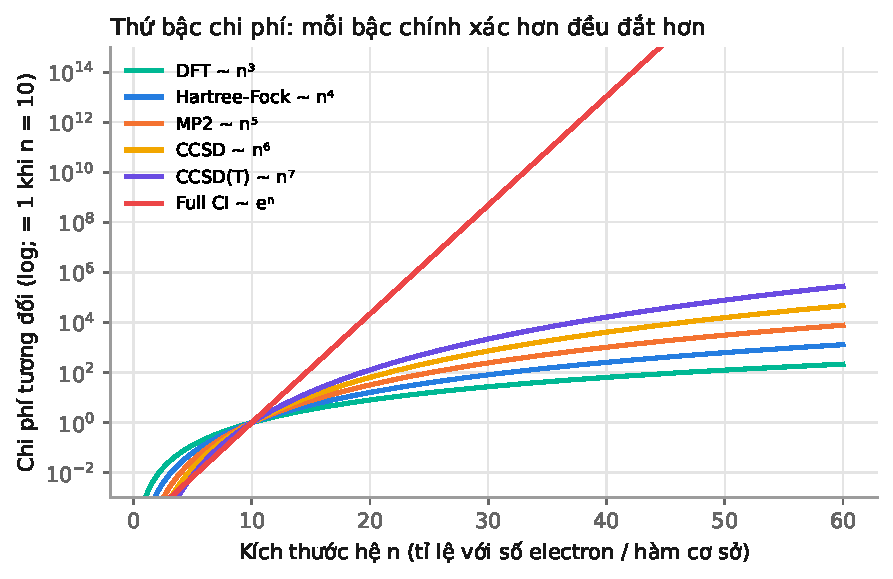
\includegraphics[width=0.8\textwidth]{03_chi_phi.pdf}
\caption{Chi phí tương đối theo kích thước hệ. Tăng kích thước 2 lần thì HF đắt hơn 16 lần, CCSD(T) đắt hơn 128 lần, còn Full CI thì tăng theo hàm mũ. (Minh họa theo bậc lý thuyết, script \code{03\_sau\_hartree\_fock.py})}
\label{fig:chiphi}
\end{figure}

\section{Kết quả cho Li}\label{sec:ketquasauhf}

\begin{chaycode}[chạy mọi phương pháp trên Li]
Script \code{03\_sau\_hartree\_fock.py} chạy UHF, MP2, CISD, CCSD, CCSD(T) và Full CI cho Li với ba tập cơ sở lõi--hóa trị cc-pCVDZ, cc-pCVTZ, cc-pCVQZ (18, 43, 84 hàm), đo thời gian chạy, rồi ngoại suy về tập cơ sở vô hạn. Cả 6 phương pháp chạy hết trong vài phút trên máy tính xách tay.
\end{chaycode}

\begin{table}[h]
\centering\small
\caption{Năng lượng của Li (Ha) tính bằng code đi kèm. Trong ngoặc: sai số so với năng lượng chính xác (mHa). Dòng cuối: phần trăm năng lượng tương quan thu được ở cc-pCVQZ. Cột CBS: HF giới hạn cộng năng lượng tương quan ngoại suy từ T và Q.}
\label{tab:sauhf}
\begin{tabular}{@{}lllll@{}}
\toprule
Phương pháp & cc-pCVDZ & cc-pCVTZ & cc-pCVQZ & CBS (T,Q) \\
\midrule
UHF & $-7.43244$ (45.62) & $-7.43270$ (45.36) & $-7.43272$ (45.34) & --- \\
MP2 & $-7.46145$ (16.61) & $-7.46987$ (8.19) & $-7.47227$ (5.79) & $-7.47401$ (4.05) \\
CISD & $-7.46602$ (12.04) & $-7.47422$ (3.84) & $-7.47633$ (1.73) & --- \\
CCSD & $-7.46602$ (12.04) & $-7.47423$ (3.83) & $-7.47633$ (1.73) & $-7.47787$ (0.19) \\
CCSD(T) & $-7.46602$ (12.04) & $-7.47425$ (3.81) & $-7.47637$ (1.69) & $-7.47791$ (0.15) \\
FCI & $-7.46603$ (12.04) & $-7.47425$ (3.81) & $-7.47637$ (1.69) & $-7.47794$ (0.12) \\
\midrule
Số hàm cơ sở & 18 & 43 & 84 & $\infty$ \\
Số định thức FCI & 2\,754 & 38\,829 & 292\,824 & --- \\
\% tương quan (QZ) & \multicolumn{4}{l}{MP2 87.2\%, CISD 96.2\%, CCSD 96.2\%, CCSD(T) 96.3\%, FCI 96.3\%} \\
\bottomrule
\end{tabular}
\end{table}


Bảng~\ref{tab:sauhf} và hình~\ref{fig:tuongquan} cho ba bài học quan trọng.

\paragraph{Bài học 1: với Li, tập cơ sở quan trọng hơn phương pháp.} Trong cùng một tập cơ sở, CISD, CCSD, CCSD(T) và FCI gần như trùng nhau (chênh nhau dưới $0.1\mHa$), vì với 3 electron, phần thiếu của CISD hay CCSD chỉ là kích thích ba, mà phần này rất nhỏ. MP2 thiếu khoảng 10\% (ở cc-pCVQZ, MP2 thu \PctMPtwoQZ\% năng lượng tương quan đúng). Nhưng cùng một phương pháp FCI, đổi từ cc-pCVDZ sang cc-pCVQZ làm năng lượng thay đổi tới $10\mHa$. Sai số còn lại của FCI/cc-pCVQZ ($\ErrFciQZ\mHa$) hoàn toàn do tập cơ sở chưa đủ lớn.

\paragraph{Bài học 2: năng lượng tương quan hội tụ chậm, nhưng ngoại suy được.} Lý thuyết (gắn với mũi nhọn Kato, mục~\ref{sec:cusp}) cho biết sai số tương quan giảm như $X^{-3}$, với $X$ là ``bậc'' tập cơ sở \cite{Helgaker1997}. Từ hai giá trị ở $X=3$ (T) và $X=4$ (Q) có thể ngoại suy về tập cơ sở vô hạn:
\[
E_{\rm corr}(\infty)\approx\frac{4^3E_{\rm corr}(4)-3^3E_{\rm corr}(3)}{4^3-3^3}.
\]
Ngoại suy FCI theo cách này thu được \PctFciCBS\% năng lượng tương quan đúng của Li, sai số chỉ còn $\ErrFciCBS\mHa$, tốt hơn độ chính xác hóa học hơn 10 lần.

\begin{figure}[h]
\centering
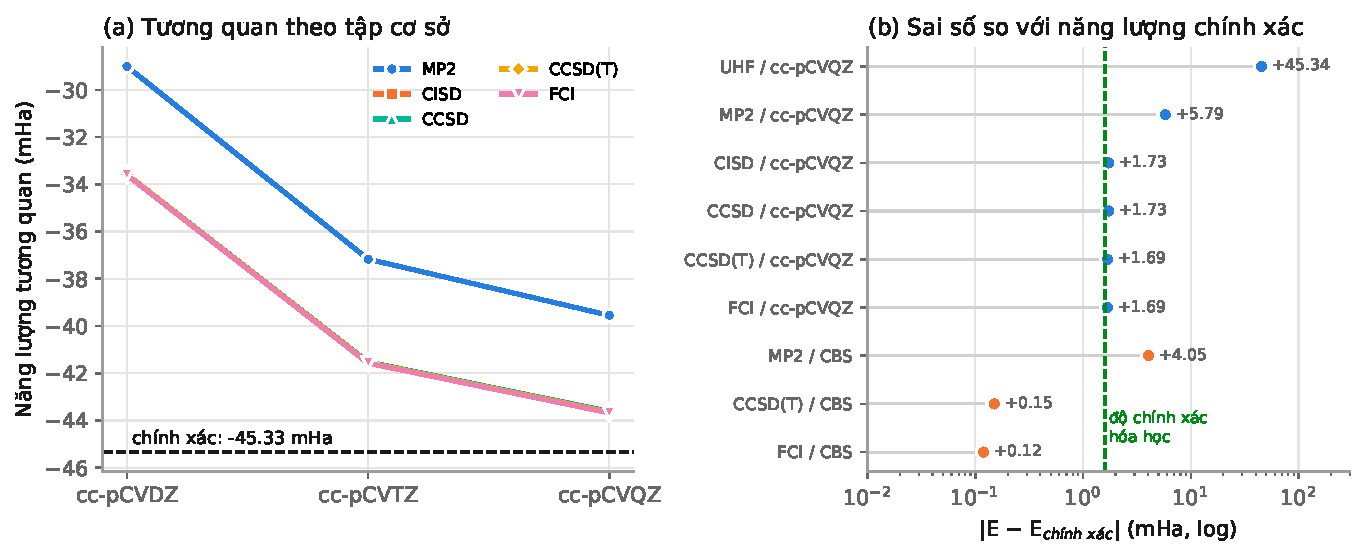
\includegraphics[width=\textwidth]{03_tuong_quan_theo_tap_co_so.pdf}
\caption{(a) Năng lượng tương quan thu được theo tập cơ sở: mọi phương pháp tương quan đầy đủ gần như trùng nhau, MP2 thấp hơn một chút; tất cả đều tiến dần về giá trị đúng $-45.33\mHa$ nhưng chậm. (b) Sai số so với năng lượng chính xác (thang log). Ngoại suy CBS kéo sai số FCI xuống dưới độ chính xác hóa học (vạch xanh lá). (Script \code{03\_sau\_hartree\_fock.py})}
\label{fig:tuongquan}
\end{figure}

\paragraph{Bài học 3: phải có hàm ``lõi''.} Tương quan của Li nằm chủ yếu ở cặp 1s$^2$ (chương~\ref{ch:hatdongnhat}). Tập cc-pVXZ chuẩn được thiết kế cho electron hóa trị, hầu như không có hàm nào ``chạm'' tới vùng lõi. Kết quả trong bảng~\ref{tab:loi} khá sốc: FCI với cc-pVQZ (55 hàm) chỉ thu \PctCorePVQZ\% năng lượng tương quan, trong khi cc-pCVQZ thu \PctCoreCVQZ\%. \emph{Loại} hàm quan trọng hơn \emph{số lượng} hàm. Một lỗi thực hành nguy hiểm khác là ``đóng băng lõi'' \en{frozen core}, một tùy chọn mặc định ở nhiều chương trình. Với Li, đóng băng 1s$^2$ là xóa sạch gần như toàn bộ tương quan.

\begin{table}[h]
\centering\small
\caption{Full CI cho Li với hai tập cơ sở cỡ QZ: không có và có hàm lõi.}
\label{tab:loi}
\begin{tabular}{@{}lrrr@{}}
\toprule
Tập cơ sở & Số hàm & $\Ecorr$ (FCI, mHa) & \% của giá trị đúng \\
\midrule
cc-pVQZ & 55 & $-17.14$ & 37.8\% \\
cc-pCVQZ & 84 & $-43.68$ & 96.3\% \\
\midrule
Giá trị đúng & $\infty$ & $-45.33$ & 100\% \\
\bottomrule
\end{tabular}
\end{table}


\subsection{Hàm sóng Full CI trông như thế nào?}
Code cũng ``mổ xẻ'' hàm sóng FCI/cc-pCVQZ của Li. Định thức HF có hệ số $c_0$ với $c_0^2=\czeroSq$: hàm sóng thật gần như hoàn toàn là ``Hartree--Fock''. Tất cả hơn 290\,000 định thức còn lại chỉ chia nhau phần nhỏ còn lại (dưới 1\%), phần lớn là kích thích đôi của cặp 1s$^2$ lên các orbital ảo. Vậy là chưa tới 1\% ``trọng lượng'' hàm sóng gánh toàn bộ $45\mHa$ năng lượng tương quan. Li là một hệ \textbf{đơn tham chiếu} \en{single-reference} điển hình: một định thức chiếm ưu thế tuyệt đối, nên các phương pháp dựa trên HF (MP2, CC) hoạt động rất tốt.

\section{Khi một định thức không đủ: phương pháp đa tham chiếu}
Có những hệ mà định thức HF \emph{không} chiếm ưu thế, ví dụ khi bẻ gãy liên kết hóa học, ở nhiều hợp chất kim loại chuyển tiếp, hay ở nguyên tử Be (cấu hình 1s$^2$2p$^2$ trộn mạnh với 1s$^2$2s$^2$). Khi đó cần \textbf{phương pháp đa tham chiếu}, phổ biến nhất là CASSCF \cite{Roos1980}: chọn một ``không gian hoạt động'' gồm vài electron và vài orbital quan trọng, làm Full CI trong không gian nhỏ đó, đồng thời tối ưu luôn các orbital. Sau đó thường thêm tương quan động bằng nhiễu loạn (CASPT2) hoặc CI (MRCI). Li ở trạng thái cơ bản không cần những phương pháp này.

\section{Đưa thẳng $r_{12}$ vào hàm sóng}
Vì sao FCI với gần 300\,000 định thức vẫn sai $\ErrFciQZ\mHa$? Vì tổ hợp các orbital mượt rất khó tạo ra mũi nhọn $\Psi\approx\Psi(0)(1+\tfrac12r_{12})$. Năm 1929, Hylleraas đưa thẳng khoảng cách $r_{12}$ vào hàm thử cho He \cite{Hylleraas1929}. Với Li, hàm Hylleraas có dạng
\[
\phi=r_{23}^{n_1}r_{31}^{n_2}r_{12}^{n_3}\,r_1^{n_4}r_2^{n_5}r_3^{n_6}\,e^{-\alpha r_1-\beta r_2-\gamma r_3}\times(\text{hàm spin}).
\]
Hiệu quả rất lớn: 60 hàm Hylleraas (Larsson 1968) đã cho sai số $0.035\mHa$ \cite{Larsson1968}, nhỏ hơn 50 lần sai số của FCI với 292\,824 định thức Gauss. Với 34\,020 hàm, Wang và cộng sự (2012) đạt 15 chữ số \cite{Wang2012}. Cái giá phải trả là các tích phân 3 electron, 4 electron trở nên cực kỳ khó, nên phương pháp Hylleraas thuần chỉ dùng được cho hệ rất nhỏ.

Phiên bản ``thực dụng'' cho phân tử là các phương pháp \textbf{F12} (hay R12): giữ khung CI/CC thông thường nhưng thêm cho mỗi cặp electron một số hạng phụ thuộc $r_{12}$ \cite{Kutzelnigg1985,Hattig2012}. CCSD(T)-F12 với tập cơ sở cỡ TZ thường chính xác ngang CCSD(T) thông thường với tập 5Z, trong khi nhanh hơn khoảng 100 lần \cite{Adler2007}.

\begin{ghinho}
\begin{itemize}
\item CI trộn định thức HF với các định thức kích thích. Full CI chính xác \emph{trong tập cơ sở}, nhưng số định thức tăng theo tổ hợp: bức tường hàm mũ lại xuất hiện.
\item CI cắt bớt (CISD) không nhất quán kích thước. MP2 ($N^5$) và Coupled Cluster ($e^{\hat T}$, CCSD $N^6$, CCSD(T) $N^7$) nhất quán kích thước nhưng không biến phân.
\item Với Li, mọi phương pháp tương quan đầy đủ gần như trùng nhau; sai số chủ yếu do tập cơ sở. Cần hàm lõi (cc-pCVXZ); ngoại suy $X^{-3}$ đưa FCI về sai số $\sim0.1\mHa$.
\item Mũi nhọn Kato làm khai triển theo orbital hội tụ chậm. Đưa $r_{12}$ vào hàm sóng (Hylleraas, F12) khắc phục điều này.
\end{itemize}
\end{ghinho}

\chapter{Lý thuyết phiếm hàm mật độ (DFT)}
\label{ch:dft}

Các chương trước đều làm việc với hàm sóng, một hàm $3N$ chiều, và đều phải trả giá trước bức tường hàm mũ. DFT đặt một câu hỏi táo bạo: \emph{có thể bỏ hẳn hàm sóng, chỉ dùng mật độ electron, một hàm 3 chiều, không?} Câu trả lời ``có, về nguyên tắc'' đã mang về giải Nobel Hóa học 1998 cho Walter Kohn. Ngày nay DFT là phương pháp được dùng nhiều nhất trong hóa học và khoa học vật liệu.

\section{Ý tưởng: bản đồ mật độ thay cho danh sách tọa độ}

\begin{eli5}[bản đồ nhiệt của sân vận động]
Muốn biết một sân vận động đông người ``cư xử'' ra sao, thay vì theo dõi tọa độ của từng người, ta chỉ cần một \emph{bản đồ nhiệt} cho biết mỗi mét vuông có bao nhiêu người. Với 50\,000 người, danh sách tọa độ có 100\,000 con số và tăng theo số người; bản đồ nhiệt thì kích thước cố định. DFT khẳng định rằng với electron ở trạng thái cơ bản, ``bản đồ mật độ'' này, nếu đọc đúng cách, chứa \emph{toàn bộ} thông tin.
\end{eli5}

\begin{congthuc}[mật độ electron]
\[
n(\vr)=N\sum_{\text{spin}}\int|\Psi(\vr,\vx_2,\ldots,\vx_N)|^2\,d\vx_2\cdots d\vx_N ,\qquad \int n(\vr)\,d\vr=N .
\]
$n(\vr)\,d\vr$ là số electron trung bình trong thể tích nhỏ $d\vr$ quanh điểm $\vr$. Dù $N$ lớn bao nhiêu, $n$ chỉ phụ thuộc 3 biến. Đây là đại lượng đo được bằng nhiễu xạ tia X.
\end{congthuc}

\subsection{Phiếm hàm là gì?}
Một \textbf{hàm} nhận một \emph{số} và trả về một số: $f(x)=x^2$. Một \textbf{phiếm hàm} \en{functional} nhận cả một \emph{hàm} và trả về một số; ta viết với ngoặc vuông $F[n]$. Ví dụ đời thường: ``lượng sơn cần dùng'' là phiếm hàm của ``hàm độ dày lớp sơn trên tường''. Ví dụ trong DFT:
\begin{itemize}
\item Số electron: $N[n]=\int n(\vr)\,d\vr$.
\item Năng lượng hút hạt nhân: $V_{\rm ext}[n]=\int\big(-\tfrac{Z}{r}\big)\,n(\vr)\,d\vr$.
\item Năng lượng Hartree, tức lực đẩy cổ điển của ``đám mây'' điện tích với chính nó: $J[n]=\tfrac12\iint\dfrac{n(\vr)\,n(\vr')}{|\vr-\vr'|}\,d\vr\,d\vr'$.
\end{itemize}

\subsection{Tiền thân: mô hình Thomas--Fermi (1927)}
Thomas và Fermi coi electron trong mỗi ô nhỏ của nguyên tử như một ``khí electron đồng nhất'', và viết động năng là $C_F\int n^{5/3}d\vr$. Mô hình cho năng lượng nguyên tử $E_{\rm TF}=-0.7687\,Z^{7/3}\Ha$ \cite{ParrGhosh1986}. Với Li, con số này là $-9.98\Ha$, sai tới 33\%. Tệ hơn, mô hình không có cấu trúc lớp vỏ, và Teller (1962) chứng minh rằng trong mô hình Thomas--Fermi \emph{không phân tử nào bền}: năng lượng phân tử luôn cao hơn tổng năng lượng các nguyên tử \cite{Teller1962}. Một lý thuyết hóa học mà không có liên kết hóa học! Phải chờ gần 40 năm để ý tưởng ``dùng mật độ'' có nền móng vững chắc.

\section{Định lý Hohenberg--Kohn (1964)}

\begin{eli5}[cuốn sách công thức không ai tìm thấy]
Hãy tưởng tượng một ``máy dò'' chỉ nhìn được bản đồ mật độ electron. Định lý Hohenberg--Kohn nói: chỉ từ bản đồ đó, máy suy ra được \emph{nguyên tử nào} đang ở đâu, và do đó suy ra được \emph{mọi thứ khác}. Có một ``công thức'' biến mật độ thành năng lượng. Nhưng định lý chỉ nói công thức đó \emph{tồn tại}, không đưa cho ta công thức. Giống như biết chắc có một cuốn sách công thức nấu ăn hoàn hảo, nhưng chưa ai tìm thấy nó.
\end{eli5}

\begin{congthuc}[hai định lý Hohenberg--Kohn]
Hamiltonian của mọi nguyên tử, phân tử có dạng $\Hhat=\hat T+\hat V_{ee}+\sum_iv(\vr_i)$. Hai số hạng đầu (động năng, đẩy nhau) giống hệt nhau cho mọi hệ; chỉ có thế ngoài $v(\vr)$ (với nguyên tử là $-Z/r$) và số electron $N$ là khác.

\textbf{Định lý 1.} Mật độ cơ bản $n_0(\vr)$ xác định duy nhất thế ngoài $v(\vr)$ (sai khác một hằng số). Do đó $n_0$ xác định $\Hhat$, và mọi tính chất của hệ.

\emph{Chứng minh phản chứng.} Giả sử hai thế $v\neq v'$ cho cùng mật độ $n$, với hai hàm sóng cơ bản $\Psi\neq\Psi'$. Áp dụng nguyên lý biến phân hai lần:
\[
E_0<\langle\Psi'|\Hhat|\Psi'\rangle=E_0'+\!\int(v-v')\,n\,d\vr,\qquad
E_0'<\langle\Psi|\Hhat'|\Psi\rangle=E_0+\!\int(v'-v)\,n\,d\vr .
\]
Cộng hai vế: $E_0+E_0'<E_0+E_0'$, vô lý. Vậy không thể có hai thế khác nhau cho cùng một mật độ.

\textbf{Định lý 2.} Tồn tại một phiếm hàm \emph{phổ quát} $F[n]$ (giống nhau cho mọi nguyên tử, phân tử) sao cho
\[
E_v[n]=F[n]+\int v(\vr)\,n(\vr)\,d\vr\;\ge\;E_0,
\]
dấu bằng khi $n$ là mật độ cơ bản đúng. Tức là có một nguyên lý biến phân cho mật độ \cite{HohenbergKohn1964}.
\end{congthuc}

Điều định lý \emph{không} nói: dạng cụ thể của $F[n]$. Mọi khó khăn của bài toán nhiều electron giờ được dồn vào việc tìm $F[n]$.

\section{Lược đồ Kohn--Sham (1965)}

Thử viết $F[n]$ trực tiếp bằng mật độ (như Thomas--Fermi) thì phần động năng sai rất nặng. Kohn và Sham nghĩ ra một mẹo thông minh \cite{KohnSham1965}.

\begin{eli5}[diễn viên đóng thế]
Thay vì giải bài toán các electron ``cãi nhau'' với nhau, Kohn và Sham thuê một đoàn ``diễn viên đóng thế'' \emph{không hề tương tác}, đặt họ trên một ``sân khấu'' (một thế hiệu dụng) được thiết kế khéo tới mức ảnh chụp đám đông diễn viên (mật độ) giống hệt ảnh chụp đám electron thật. Diễn viên không tương tác thì dễ mô tả: mỗi người chiếm một orbital, và động năng của họ tính chính xác được. Mọi phần khó, tức là việc electron né nhau, được gói vào \emph{một} số hạng duy nhất: năng lượng trao đổi--tương quan $E_{xc}$.
\end{eli5}

\begin{congthuc}[phương trình Kohn--Sham]
Năng lượng toàn phần được tách thành
\[
E[n]=\underbrace{T_s[n]}_{\text{động năng hệ không tương tác}}+\underbrace{\int v_{\rm ext}\,n\,d\vr}_{\text{hút hạt nhân}}+\underbrace{J[n]}_{\text{Hartree}}+\underbrace{E_{xc}[n]}_{\text{mọi thứ còn lại}} .
\]
Các orbital Kohn--Sham thỏa phương trình kiểu Schrödinger một electron:
\[
\Big[-\tfrac12\nabla^2+v_{\rm ext}(\vr)+v_H(\vr)+v_{xc}(\vr)\Big]\varphi_i(\vr)=\varepsilon_i\varphi_i(\vr),\qquad n(\vr)=\sum_{i}^{\text{chiếm}}|\varphi_i(\vr)|^2,
\]
với thế Hartree $v_H(\vr)=\int\frac{n(\vr')}{|\vr-\vr'|}d\vr'$ và thế trao đổi--tương quan $v_{xc}(\vr)=\delta E_{xc}/\delta n(\vr)$ (đạo hàm phiếm hàm: ``thêm một chút mật độ tại $\vr$ thì $E_{xc}$ đổi bao nhiêu'').
\begin{itemize}
\item $E_{xc}=(T-T_s)+(V_{ee}-J)$: gồm phần động năng tương quan, và phần tương tác electron ``phi cổ điển'' (trao đổi, tương quan, và việc sửa lỗi electron tự đẩy chính mình chứa trong $J$).
\item Vì thế phụ thuộc mật độ, mật độ phụ thuộc thế, nên phải giải lặp tới tự hợp, đúng như Hartree--Fock.
\item Với Li (phân cực spin): orbital 1s$\uparrow$, 2s$\uparrow$, 1s$\downarrow$; mỗi spin có thế $v_{xc}^\sigma$ riêng.
\end{itemize}
\end{congthuc}

Nếu biết $E_{xc}$ chính xác, Kohn--Sham cho năng lượng và mật độ \emph{chính xác}. Với Li, $E_{xc}\approx-1.83\Ha$ trên tổng $-7.48\Ha$; riêng phần tương quan chỉ $-0.045\Ha$. Toàn bộ nghệ thuật của DFT hiện đại là xấp xỉ $E_{xc}$.

\begin{hieulam}[orbital Kohn--Sham là orbital ``thật'']
Định thức dựng từ orbital Kohn--Sham \emph{không} phải hàm sóng thật của hệ; orbital KS là công cụ phụ trợ để tính đúng mật độ. Chỉ có một ngoại lệ quan trọng: với phiếm hàm chính xác, năng lượng orbital cao nhất bằng đúng trừ năng lượng ion hóa, $\varepsilon_{\rm HOMO}=-I$ (định lý năng lượng ion hóa \cite{PPLB1982}). Với Li, thế xc chính xác dựng ngược từ mật độ rất chính xác cho $\varepsilon_{\rm HOMO}=-0.197\Ha$, so với $-I=-0.198\Ha$ \cite{Kanungo2023}.
\end{hieulam}

\section{Bậc thang Jacob của các phiếm hàm}

Perdew (2001) mô tả các phiếm hàm xấp xỉ như những bậc trên \textbf{``chiếc thang Jacob''} \cite{PerdewSchmidt2001}, đi từ ``thế giới Hartree'' (không có trao đổi--tương quan) lên ``thiên đường độ chính xác hóa học''. Mỗi bậc thêm một ``nguyên liệu'' mới:

\begin{table}[h]
\centering\small
\caption{Bậc thang Jacob \cite{PerdewSchmidt2001}.}
\label{tab:jacob}
\begin{tabularx}{\textwidth}{@{}clXl@{}}
\toprule
Bậc & Tên & Nguyên liệu thêm vào & Ví dụ \\
\midrule
1 & LDA (LSDA) & mật độ tại chỗ $n_\uparrow(\vr),n_\downarrow(\vr)$ & SVWN, PW92 \\
2 & GGA & thêm độ dốc của mật độ $\nabla n$ & PBE, BLYP \\
3 & meta-GGA & thêm mật độ động năng $\tau=\tfrac12\sum_i|\nabla\varphi_i|^2$ & TPSS, SCAN, r$^2$SCAN \\
4 & hybrid & thêm một phần trao đổi chính xác (kiểu HF) & B3LYP, PBE0 \\
5 & double hybrid, RPA & thêm cả orbital ảo (kiểu MP2) & B2PLYP \\
\bottomrule
\end{tabularx}
\end{table}

\begin{congthuc}[các bậc chính]
\textbf{LDA:} $E_{xc}^{\rm LDA}=\int n(\vr)\,\varepsilon_{xc}^{\rm unif}\big(n(\vr)\big)\,d\vr$. Tại mỗi điểm, dùng năng lượng của \emph{khí electron đồng nhất} có cùng mật độ. Phần trao đổi có công thức chính xác $\varepsilon_x^{\rm unif}=-\tfrac34(3n/\pi)^{1/3}$; phần tương quan lấy từ mô phỏng Monte Carlo lượng tử của Ceperley và Alder (1980) \cite{CeperleyAlder1980}, được khớp thành công thức bởi Vosko--Wilk--Nusair (VWN) và Perdew--Wang.

\textbf{GGA:} $E_{xc}^{\rm GGA}=\int n\,\varepsilon_x^{\rm unif}(n)\,F_{xc}(n,s)\,d\vr$ với độ dốc rút gọn $s=|\nabla n|/(2k_Fn)$. PBE \cite{PBE1996} chọn ``hệ số tăng cường'' $F_{xc}$ chỉ từ các ràng buộc vật lý chính xác, không khớp dữ liệu thực nghiệm.

\textbf{Hybrid:} trộn một phần trao đổi HF. Ví dụ PBE0: $E_{xc}^{\rm PBE0}=E_{xc}^{\rm PBE}+\tfrac14\big(E_x^{\rm HF}-E_x^{\rm PBE}\big)$ \cite{AdamoBarone1999}. B3LYP \cite{Becke1993,Stephens1994} dùng 3 tham số khớp từ dữ liệu thực nghiệm (20\% trao đổi HF).
\end{congthuc}

Có hai ``triết lý'' xây dựng phiếm hàm: \emph{thỏa các ràng buộc chính xác} (PBE, SCAN: tham số là hằng số vật lý) và \emph{khớp dữ liệu thực nghiệm} (B3LYP, họ Minnesota). Thang Jacob chỉ thể hiện xu hướng trung bình, không phải đảm bảo cho từng tính chất. Ngay với Li, ta sẽ thấy phiếm hàm bậc cao hơn không luôn tốt hơn.

\section{DFT cho Li: kết quả}

\begin{chaycode}[sáu phiếm hàm, ba hệ]
Script \code{04\_dft.py} tính Li, Li$^+$ và nguyên tử H với LDA (SVWN5), PBE, BLYP, r$^2$SCAN, B3LYP, PBE0 và so với HF, dùng Kohn--Sham không hạn chế với tập cơ sở aug-cc-pCVQZ. Hai bẫy thực hành do subagent nghiên cứu phát hiện: trong PySCF, \code{xc="lda"} \emph{chỉ có phần trao đổi}, muốn có tương quan phải viết \code{"lda,vwn"}; và phiếm hàm SCAN gốc không hội tụ với Li, nên dùng phiên bản ổn định hơn là r$^2$SCAN \cite{Lehtola2023}.
\end{chaycode}

\begin{table}[h]
\centering\small
\caption{Li với các phiếm hàm (tập cơ sở aug-cc-pCVQZ, tính bằng code đi kèm). Cột cuối: nguyên tử H, nơi đáp án đúng là $-0.5\Ha$; mọi sai số ở đó là lỗi tự tương tác.}
\label{tab:dft}
\begin{tabular}{@{}llrrrr@{}}
\toprule
Phương pháp & Bậc & $E-E_{\text{chính xác}}$ & IE ($\Delta$SCF) & $-\varepsilon_{\rm HOMO}$ & H: $E+0.5$ \\
 & & (mHa) & (eV) & (eV) & (mHa) \\
\midrule
Hartree-Fock & HF & $+45.3$ & 5.343 & 5.343 & $+0.0$ \\
LDA (SVWN5) & LDA & $+134.1$ & 5.473 & 3.165 & $+21.3$ \\
PBE & GGA & $+15.9$ & 5.589 & 3.227 & $+0.0$ \\
BLYP & GGA & $-4.6$ & 5.530 & 3.030 & $+2.1$ \\
r²SCAN & meta-GGA & $-1.6$ & 5.391 & 3.263 & $-0.2$ \\
B3LYP & hybrid & $-14.9$ & 5.627 & 3.649 & $-2.4$ \\
PBE0 & hybrid & $+10.9$ & 5.571 & 3.831 & $-1.3$ \\
\midrule
Chính xác / thực nghiệm & & 0 & 5.392 / 5.392 & 5.392 & 0 \\
\bottomrule
\end{tabular}
\end{table}


\begin{figure}[h]
\centering
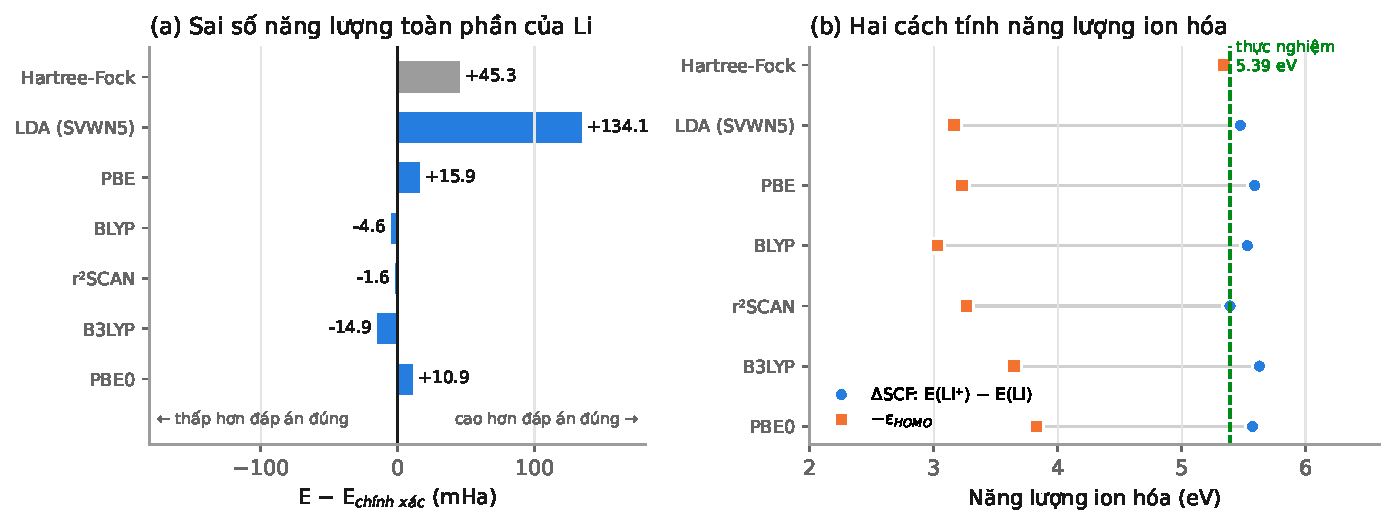
\includegraphics[width=\textwidth]{04_dft_li.pdf}
\caption{(a) Sai số năng lượng toàn phần của Li với từng phiếm hàm (thanh xám: HF). Một số phiếm hàm cho năng lượng \emph{thấp hơn} đáp án đúng. (b) Năng lượng ion hóa tính bằng hiệu năng lượng (tròn xanh) và bằng $-\varepsilon_{\rm HOMO}$ (vuông cam); vạch xanh lá là thực nghiệm. (Script \code{04\_dft.py})}
\label{fig:dftli}
\end{figure}

Bảng~\ref{tab:dft} và hình~\ref{fig:dftli} cho bốn bài học.

\paragraph{1. LDA sai năng lượng toàn phần rất nhiều.} LDA cao hơn đáp án $\ErrLDA\mHa$ (khoảng 3.7\,eV), tệ hơn cả HF. Nguyên tử khác xa một ``khí electron đồng nhất''.

\paragraph{2. DFT xấp xỉ không cho cận trên.} B3LYP cho năng lượng thấp hơn đáp án đúng ($\ErrBthreeLYP\mHa$). Khác với HF hay CI, năng lượng DFT với phiếm hàm xấp xỉ \emph{không} tuân theo nguyên lý biến phân đối với năng lượng thật. ``Thấp hơn'' không có nghĩa ``tốt hơn''.

\paragraph{3. Hiệu năng lượng tốt hơn năng lượng.} Dù LDA sai năng lượng toàn phần tới $\ErrLDA\mHa$, năng lượng ion hóa tính bằng hiệu $E(\text{Li}^+)-E(\text{Li})$ chỉ là $\IEdeltaLDA\eV$, so với thực nghiệm $5.39\eV$. Sai số của Li và Li$^+$ (cùng lõi 1s$^2$) \textbf{triệt tiêu nhau}. Đây là lý do DFT hữu ích trong hóa học: hóa học quan tâm tới \emph{hiệu} năng lượng (năng lượng phản ứng, liên kết), và sai số thường triệt tiêu một phần.

Riêng r$^2$SCAN cho năng lượng ion hóa trùng thực nghiệm tới $0.01\eV$. Đừng vội coi đó là thành công: với Li, các phiếm hàm meta-GGA rất nhạy với lưới tích phân và tập cơ sở, và nghiên cứu chuẩn của Lehtola (2023) thậm chí không đạt được hội tụ SCF cho r$^2$SCAN ở giới hạn tập cơ sở \cite{Lehtola2023}. Sự trùng khớp này nhiều khả năng là ngẫu nhiên.

\paragraph{4. Năng lượng orbital cao nhất sai nặng.} Với phiếm hàm chính xác, $-\varepsilon_{\rm HOMO}$ phải bằng năng lượng ion hóa $5.39\eV$. LDA cho $\HomoLDA\eV$, PBE $\HomoPBE\eV$, B3LYP $\HomoBthreeLYP\eV$: thiếu khoảng 40\%. Trong khi đó HF (định lý Koopmans) cho $\HomoHF\eV$. Thủ phạm là \textbf{lỗi tự tương tác}.

\section{Lỗi tự tương tác}

\begin{eli5}[sợ chính cái bóng của mình]
Một electron đơn lẻ không thể tự đẩy chính mình. Nhưng số hạng Hartree $J[n]$ tính lực đẩy của \emph{toàn bộ} đám mây điện tích lên chính nó, kể cả phần ``electron tự đẩy mình''. Với phiếm hàm chính xác, phần trao đổi xóa sạch sự tự đẩy giả tạo này (như Hartree--Fock làm được, chương~\ref{ch:hf}). Phiếm hàm xấp xỉ chỉ xóa được phần lớn, giống như một người soi gương rồi sợ chính cái bóng của mình.
\end{eli5}

Phép thử sạch nhất là nguyên tử H: chỉ có một electron, không có tương quan, đáp án đúng $E=-0.5\Ha$ và $-\varepsilon_{\rm HOMO}=13.6\eV$. Cột cuối của bảng~\ref{tab:dft} cho thấy LDA sai $\HerrLDA\mHa$, PBE sai $\HerrPBE\mHa$ (gần đúng nhờ may mắn: sai số trao đổi và tương quan gần triệt tiêu nhau), B3LYP sai $\HerrBthreeLYP\mHa$, trong khi HF chỉ sai $\HerrHF\mHa$ (do tập cơ sở). Về năng lượng orbital, $-\varepsilon$ của H theo LDA chỉ khoảng $\HhomoLDA\eV$, theo PBE $\HhomoPBE\eV$, so với $13.6\eV$. Thế trao đổi--tương quan của LDA và GGA tắt quá nhanh khi ra xa (theo hàm mũ thay vì $-1/r$), làm electron ngoài cùng bị ``giữ'' quá lỏng. Đây là gốc rễ của nhiều thất bại khác của DFT: khe năng lượng của chất bán dẫn bị đánh giá thấp, điện tích bị trải quá rộng \cite{Cohen2008}.

\begin{figure}[h]
\centering
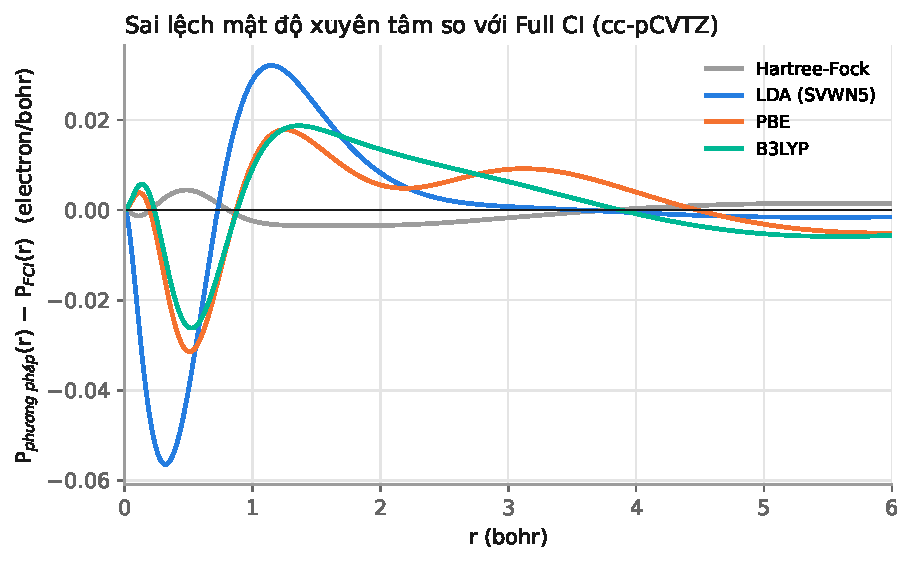
\includegraphics[width=0.8\textwidth]{04_sai_lech_mat_do.pdf}
\caption{Mật độ xuyên tâm của HF, LDA, PBE và B3LYP trừ đi mật độ Full CI (gần như chính xác), cùng tập cơ sở cc-pCVTZ. Cả ba phiếm hàm đều ``rút'' mật độ khỏi đỉnh lớp 1s ($r\approx0.3$--$0.5\bohr$) và dồn ra vùng giữa hai lớp vỏ ($r\approx1$--$2\bohr$), LDA mạnh nhất. Tổng sai lệch $\int|\Delta P|\,dr$ là 0.014 electron cho HF và khoảng 0.06 electron cho cả ba phiếm hàm: với nguyên tử nhỏ này, mật độ HF gần mật độ chính xác hơn mật độ DFT. (Script \code{04\_dft.py})}
\label{fig:matdodft}
\end{figure}

\section{Các thất bại khác đã biết}
\begin{itemize}
\item \textbf{Lực phân tán (van der Waals):} lực hút yếu giữa các phân tử trung hòa đến từ dao động mật độ tương quan ở hai nơi xa nhau. LDA và GGA chỉ ``nhìn'' mật độ tại chỗ nên bỏ sót. Thực tế người ta cộng thêm hiệu chỉnh kiểu DFT-D3 \cite{Grimme2010}.
\item \textbf{Tương quan mạnh:} khi nhiều cấu hình gần suy biến (kéo giãn liên kết, nhiều oxit kim loại chuyển tiếp), một định thức Kohn--Sham với phiếm hàm xấp xỉ thất bại. Đây là bài toán ``ít được giải quyết nhất'' của DFT \cite{Mardirossian2017}.
\item \textbf{Khe năng lượng:} LDA và GGA đánh giá thấp khe năng lượng của chất bán dẫn và cách điện khoảng 40\% \cite{PerdewLevy1983}.
\item \textbf{Không có cách cải thiện có hệ thống:} khác với chuỗi HF $\to$ MP2 $\to$ CCSD $\to$ CCSD(T) $\to$ FCI, không có ``núm vặn'' nào đảm bảo phiếm hàm mới tốt hơn cho mọi hệ. Có hàng trăm phiếm hàm khác nhau.
\end{itemize}

\section{Vì sao DFT vẫn thống trị?}
\begin{itemize}
\item \textbf{Chi phí:} Kohn--Sham với LDA hoặc GGA tăng như $N^3$ theo kích thước hệ, rẻ hơn HF một bậc, và rất rẻ so với CCSD(T) ($N^7$). DFT xử lý được hàng trăm tới hàng nghìn nguyên tử.
\item \textbf{Độ chính xác ``đủ dùng'':} với hiệu năng lượng (phản ứng, cấu trúc, tần số dao động), các hybrid tốt thường sai vài kcal/mol.
\item \textbf{Tầm ảnh hưởng:} theo danh sách 100 bài báo được trích dẫn nhiều nhất mọi thời đại của tạp chí Nature (2014), 12 bài liên quan tới DFT; bài của Lee--Yang--Parr (1988) đứng thứ 7 và bài B3 của Becke (1993) đứng thứ 8 \cite{VanNoorden2014}.
\end{itemize}

\begin{ghinho}
\begin{itemize}
\item DFT thay hàm sóng $3N$ chiều bằng mật độ 3 chiều. Định lý Hohenberg--Kohn đảm bảo mật độ chứa mọi thông tin, nhưng không cho dạng của phiếm hàm.
\item Kohn--Sham dùng một hệ ``diễn viên'' không tương tác có cùng mật độ; mọi phần khó gói vào $E_{xc}$, thứ phải xấp xỉ (LDA, GGA, meta-GGA, hybrid\ldots).
\item Với Li: năng lượng toàn phần có thể sai nhiều (LDA $\ErrLDA\mHa$) và có thể thấp hơn đáp án (B3LYP), nhưng hiệu năng lượng như năng lượng ion hóa thì tốt nhờ triệt tiêu sai số.
\item Lỗi tự tương tác làm $-\varepsilon_{\rm HOMO}$ của LDA/GGA thiếu khoảng 40\% năng lượng ion hóa. Không có cách cải thiện phiếm hàm có hệ thống như chuỗi CC.
\end{itemize}
\end{ghinho}

\chapter{Monte Carlo lượng tử: giải bằng ngẫu nhiên}
\label{ch:qmc}

Các chương trước đều \emph{viết} hàm sóng ra dưới dạng tổ hợp các hàm cơ sở, và đều gặp bức tường tổ hợp hoặc phải xấp xỉ. Monte Carlo lượng tử (QMC) đi một con đường khác: \emph{không lưu hàm sóng}, mà chỉ lấy mẫu những cấu hình electron ``điển hình'' một cách ngẫu nhiên. Phương pháp này làm việc trực tiếp với tọa độ thật của electron, không cần tập cơ sở, và có thể dùng hàm sóng chứa $r_{12}$ tường minh.

\section{Ý tưởng Monte Carlo}

\begin{eli5}[đo diện tích hồ bằng cách ném đá]
Muốn đo diện tích một cái hồ có hình thù kỳ quặc nằm trong một mảnh đất hình vuông, bạn ném thật nhiều viên đá ngẫu nhiên vào mảnh đất và đếm tỉ lệ viên rơi xuống nước. Tỉ lệ đó nhân với diện tích mảnh đất cho diện tích hồ. Ném càng nhiều, kết quả càng chính xác.

Điều kỳ diệu: sai số chỉ phụ thuộc vào \emph{số viên đá}, không phụ thuộc vào \emph{số chiều} của ``mảnh đất''. Hàm sóng Li sống trong 9 chiều, Fe trong 78 chiều, nhưng sai số Monte Carlo vẫn giảm như $1/\sqrt{\text{số mẫu}}$. Đây chính là cách đi vòng qua bức tường hàm mũ.

\emph{Chỗ ví dụ ``gãy'':} ném đá \emph{đều} khắp nơi rất lãng phí khi hàm sóng chỉ lớn ở một vùng nhỏ. QMC ném đá \emph{thông minh}: nhiều hơn ở chỗ electron hay có mặt.
\end{eli5}

\begin{congthuc}[sai số Monte Carlo]
Trung bình của $M$ mẫu ngẫu nhiên độc lập có sai số chuẩn
\[
\sigma_{\bar x}=\frac{\sigma}{\sqrt M},
\]
với $\sigma$ là độ lệch chuẩn của một mẫu. Muốn giảm sai số 10 lần phải tăng số mẫu 100 lần, nhưng con số này \emph{không phụ thuộc số chiều} của tích phân. Với lưới đều trong $d$ chiều, sai số giảm như $M^{-k/d}$ (với $k$ là bậc chính xác của quy tắc tích phân), nên lưới hoàn toàn vô dụng khi $d$ lớn.
\end{congthuc}

\section{Monte Carlo biến phân (VMC)}

\begin{congthuc}[năng lượng như một trung bình]
Với hàm thử $\Psi_T(\mathbf R)$, trong đó $\mathbf R=(\vr_1,\vr_2,\vr_3)$ là vị trí cả ba electron, năng lượng biến phân viết được thành
\[
E[\Psi_T]=\frac{\int|\Psi_T(\mathbf R)|^2\,E_L(\mathbf R)\,d\mathbf R}{\int|\Psi_T(\mathbf R)|^2\,d\mathbf R},\qquad
E_L(\mathbf R)=\frac{\Hhat\Psi_T(\mathbf R)}{\Psi_T(\mathbf R)} .
\]
\begin{itemize}
\item $|\Psi_T|^2/\!\int|\Psi_T|^2$ là một \textbf{phân bố xác suất} trên không gian 9 chiều: xác suất thấy ba electron ở ba vị trí $\vr_1,\vr_2,\vr_3$.
\item $E_L$ là \textbf{năng lượng cục bộ} \en{local energy}: một con số tính được tại từng cấu hình $\mathbf R$.
\item Vậy $E$ chỉ là \emph{trung bình} của $E_L$ trên các cấu hình lấy mẫu theo $|\Psi_T|^2$: $E\approx\frac1M\sum_{k=1}^M E_L(\mathbf R_k)$.
\end{itemize}
\textbf{Tính chất ``phương sai bằng không'':} nếu $\Psi_T$ là hàm sóng chính xác thì $\Hhat\Psi_T=E_0\Psi_T$, nên $E_L(\mathbf R)=E_0$ \emph{tại mọi điểm}. Mọi mẫu cho cùng một giá trị và sai số thống kê bằng 0. Hàm thử càng tốt, $E_L$ càng ít dao động. Đây là một ``đồng hồ đo chất lượng'' rất hữu ích.
\end{congthuc}

\subsection{Thuật toán Metropolis}
Làm sao lấy mẫu theo một phân bố 9 chiều phức tạp như $|\Psi_T|^2$? Thuật toán Metropolis (1953) \cite{Metropolis1953} cho một ``người đi bộ ngẫu nhiên'' \en{walker} đi lang thang sao cho lâu dần, thời gian nó ở mỗi vùng tỉ lệ với $|\Psi_T|^2$:
\begin{enumerate}
\item Từ cấu hình hiện tại $\mathbf R$, đề xuất bước mới $\mathbf R'=\mathbf R+\boldsymbol\delta$ ($\boldsymbol\delta$ ngẫu nhiên nhỏ).
\item Chấp nhận bước với xác suất $\min\!\big(1,\,|\Psi_T(\mathbf R')|^2/|\Psi_T(\mathbf R)|^2\big)$; nếu không chấp nhận thì đứng yên.
\item Lặp lại. Sau một thời gian ``làm nóng'', các cấu hình là mẫu của $|\Psi_T|^2$.
\end{enumerate}
Điểm hay: chỉ cần \emph{tỉ số} $\Psi_T(\mathbf R')/\Psi_T(\mathbf R)$, không cần biết hằng số chuẩn hóa (một tích phân 9 chiều mà ta không tính được).

\begin{figure}[h]
\centering
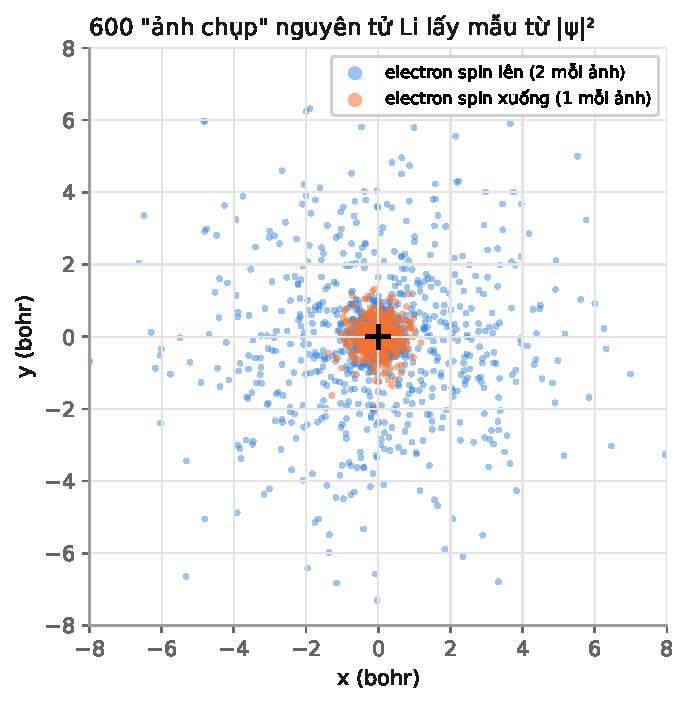
\includegraphics[width=0.6\textwidth]{05_dam_may_electron.pdf}
\caption{600 ``ảnh chụp'' nguyên tử Li do thuật toán Metropolis lấy mẫu từ $|\Psi_T|^2$ (chiếu xuống mặt phẳng $xy$). Mỗi ảnh có 2 electron spin lên (xanh) và 1 electron spin xuống (cam). Electron spin xuống hầu như luôn ở lớp trong; hai electron spin lên thường có một ở lớp trong và một ở lớp ngoài: đúng bức tranh 1s$^2$2s. (Script \code{05\_monte\_carlo\_luong\_tu.py})}
\label{fig:dammay}
\end{figure}

\subsection{Hàm thử Slater--Jastrow}
Hàm thử phổ biến nhất trong QMC là \textbf{định thức Slater nhân thừa số Jastrow} \cite{Jastrow1955}:
\[
\Psi_T(\mathbf R)=D_\uparrow(\vr_1,\vr_2)\,D_\downarrow(\vr_3)\,e^{J(\mathbf R)} .
\]
Phần định thức lo việc phản đối xứng (và nguyên lý Pauli). Phần Jastrow $e^J$ luôn dương, nên không làm thay đổi dấu của hàm sóng, nhưng mô tả việc các electron ``né nhau''. Đây đúng là thứ Hartree--Fock thiếu.

\begin{congthuc}[hàm thử dùng trong code]
\begin{itemize}
\item Orbital: $\phi_1(r)=e^{-z_1r}$ (kiểu 1s) và $\phi_2(r)=(1-cr)e^{-z_2r}$ (kiểu 2s, có một nút), với $c=z_1-z_2$.
\item Định thức spin lên: $D_\uparrow=\phi_1(r_1)\phi_2(r_2)-\phi_1(r_2)\phi_2(r_1)$. Spin xuống: $D_\downarrow=\phi_1(r_3)$.
\item Jastrow electron--electron: $J_{ee}=\sum_{i<j}\dfrac{a_{ij}\,r_{ij}}{1+b\,r_{ij}}$, với $a_{ij}=\tfrac12$ cho cặp ngược spin và $\tfrac14$ cho cặp cùng spin. Khi $r_{ij}\to0$, $e^{J}\approx1+a_{ij}r_{ij}$: đúng điều kiện cusp của Kato (mục~\ref{sec:cusp}).
\item Jastrow electron--hạt nhân: $J_{en}=-\sum_i\dfrac{(Z-z_1)\,r_i}{1+d\,r_i}$. Cộng với đạo hàm của orbital tại gốc ($-z_1$), đạo hàm log của $\Psi_T$ khi electron chạm hạt nhân đúng bằng $-Z$: thỏa cusp electron--hạt nhân.
\end{itemize}
Bốn tham số $(z_1,z_2,d,b)$ được tối ưu để năng lượng nhỏ nhất. Gradient và laplacian của $\Psi_T$ (cần cho $E_L$) được tính bằng công thức giải tích và kiểm tra lại bằng sai phân hữu hạn (khớp tới $10^{-7}$).
\end{congthuc}

\begin{hieulam}[bỏ qua điều kiện cusp]
Phiên bản đầu tiên của code \emph{không} thỏa điều kiện cusp electron--hạt nhân. VMC vẫn chạy được, nhưng năng lượng cục bộ $E_L$ tiến ra vô cùng mỗi khi một electron tới sát hạt nhân. Với DMC (mục sau), điều này làm quần thể walker ``bùng nổ'' và cho năng lượng $-50\Ha$, một con số vô nghĩa. Điều kiện cusp không phải chi tiết toán học cho đẹp: nó quyết định phương pháp có chạy được hay không.
\end{hieulam}

Kết quả VMC (bảng~\ref{tab:qmc}): chỉ dùng định thức Slater với các orbital đơn giản chưa tối ưu, $E=\EvmcSlater\Ha$, còn cao hơn cả giới hạn Hartree--Fock. Thêm Jastrow và tối ưu 4 tham số, $E=\Evmc\Ha$, thu \PctVmc\% năng lượng tương quan, chỉ với 4 tham số. Để so sánh: Full CI cần gần 300\,000 định thức mới thu được khoảng 96\%.

\section{Monte Carlo khuếch tán (DMC)}

VMC chỉ tốt bằng hàm thử. DMC đi xa hơn: nó \emph{tự động} lọc hàm thử để tiến về trạng thái cơ bản thật.

\begin{eli5}[mực loang trong nước]
Thay $t$ trong phương trình Schrödinger phụ thuộc thời gian bằng ``thời gian ảo'' $\tau=it$. Phương trình trở thành giống phương trình \emph{khuếch tán}, mô tả mực loang trong nước, cộng thêm một số hạng ``sinh--diệt''. Thả một đám walker; mỗi walker khuếch tán ngẫu nhiên. Walker ở vùng thế năng thấp (gần hạt nhân) thì ``sinh sôi'' (nhân bản), walker ở vùng thế năng cao thì ``chết'' (biến mất). Sau đủ lâu, đám walker phân bố đúng theo hàm sóng của trạng thái cơ bản, bất kể ban đầu thả thế nào.
\end{eli5}

\begin{congthuc}[phép chiếu bằng thời gian ảo]
Khai triển hàm ban đầu theo các trạng thái riêng, $\Psi(0)=\sum_n c_n\Psi_n$, rồi ``tiến hóa'' theo thời gian ảo:
\[
\Psi(\tau)=e^{-(\Hhat-E_T)\tau}\Psi(0)=\sum_n c_n\,e^{-(E_n-E_T)\tau}\,\Psi_n
\;\xrightarrow{\tau\to\infty}\;c_0\,e^{-(E_0-E_T)\tau}\,\Psi_0 .
\]
Mọi trạng thái kích thích tắt dần theo $e^{-(E_n-E_0)\tau}$ nhanh hơn trạng thái cơ bản, nên chỉ còn lại $\Psi_0$. Năng lượng thử $E_T$ được điều chỉnh liên tục để giữ số walker ổn định. Phương trình tương ứng
\[
-\frac{\partial\Psi}{\partial\tau}=-\tfrac12\nabla^2\Psi+(V-E_T)\Psi
\]
có hai phần: $-\tfrac12\nabla^2$ là khuếch tán (walker đi ngẫu nhiên), $(V-E_T)$ là sinh--diệt (walker nhân bản hay biến mất với trọng số $e^{-(V-E_T)\delta\tau}$). Thực tế người ta dùng \textbf{lấy mẫu theo tầm quan trọng} \en{importance sampling}: walker còn ``trôi'' theo vận tốc $\nabla\ln|\Psi_T|$ về phía hàm thử lớn, và trọng số dùng $E_L$ thay cho $V$, nên dao động nhỏ hơn rất nhiều \cite{Reynolds1982,Umrigar1993}.
\end{congthuc}

\section{Bài toán dấu và gần đúng nút cố định}

DMC coi hàm sóng như \emph{mật độ} của walker, mà mật độ thì không âm. Nhưng hàm sóng fermion bắt buộc đổi dấu (phản đối xứng)! Nếu cứ để walker tự do, đám walker sẽ hội tụ về trạng thái thấp nhất \emph{không có ràng buộc đối xứng}, tức là ``trạng thái boson'', như cái bẫy boson ở hình~\ref{fig:bacthang}.

\begin{eli5}[cộng những số khổng lồ trái dấu]
Muốn tính một con số nhỏ bằng cách cộng hàng triệu số dương khổng lồ với hàng triệu số âm khổng lồ gần bằng chúng: chỉ một sai số nhỏ trong mỗi số cũng làm kết quả cuối cùng vô nghĩa. Mô phỏng fermion bằng walker mang dấu $+$ và $-$ gặp đúng tình trạng này: tín hiệu (hiệu của hai đám walker) tắt dần theo hàm mũ, còn nhiễu thì không. Đó là \textbf{bài toán dấu} \en{sign problem}.
\end{eli5}

Troyer và Wiese (2005) đã chứng minh rằng một lời giải tổng quát cho bài toán dấu sẽ kéo theo việc giải được cả lớp bài toán NP-khó \cite{TroyerWiese2005}, nên khó có hy vọng tìm ra ``thuốc chữa'' tổng quát. Cách làm thực tế là \textbf{gần đúng nút cố định} \en{fixed-node approximation} \cite{Reynolds1982}: lấy \emph{nút} (mặt $\Psi_T=0$) của hàm thử làm ``tường'', cấm walker đi xuyên qua. Trong mỗi vùng kẹp giữa các nút, hàm sóng không đổi dấu nên DMC chạy bình thường. Kết quả là năng lượng thấp nhất có cùng mặt nút với $\Psi_T$. Đây vẫn là một cận trên biến phân: nếu nút đúng thì năng lượng đúng, nếu nút sai thì năng lượng cao hơn một chút.

Với hàm thử của chúng ta, nút có dạng rất đơn giản. $D_\uparrow=0$ khi $\phi_2(r_1)/\phi_1(r_1)=\phi_2(r_2)/\phi_1(r_2)$. Vì tỉ số $\phi_2/\phi_1=(1-cr)e^{(z_1-z_2)r}$ là hàm giảm đơn điệu theo $r$ (có thể kiểm tra bằng đạo hàm), nút chính là mặt $r_1=r_2$: \emph{hai electron cùng spin cách hạt nhân bằng nhau}. Đây cũng chính là nút của hàm Hartree--Fock, và các nghiên cứu cho thấy nó trùng gần như hoàn toàn với nút của hàm sóng chính xác \cite{Bressanini2001,Brown2007}. (Với Be, chỉ thêm một electron, nút của Hartree--Fock đã sai về hình dạng tô-pô và gây sai số khoảng $10\mHa$.)

\section{Kết quả cho Li}

\begin{chaycode}[QMC trong 300 dòng numpy]
Script \code{05\_monte\_carlo\_luong\_tu.py} cài đặt VMC (Metropolis, tối ưu tham số bằng lấy mẫu tương quan) và DMC (lấy mẫu theo tầm quan trọng, chấp nhận Metropolis--Hastings, nút cố định, giới hạn vận tốc trôi theo Umrigar và cộng sự \cite{Umrigar1993}) với 4000 walker. DMC chạy với 4 bước thời gian $\tau$ khác nhau rồi ngoại suy về $\tau\to0$, vì phép chia thời gian thành các bước hữu hạn gây ra một sai số hệ thống tỉ lệ với $\tau$.
\end{chaycode}

\begin{table}[h]
\centering\small
\caption{Kết quả Monte Carlo lượng tử tự viết cho Li (script \code{05\_monte\_carlo\_luong\_tu.py}). Sai số thống kê ($1\sigma$) ghi sau dấu $\pm$.}
\label{tab:qmc}
\begin{tabular}{@{}lrrr@{}}
\toprule
Phương pháp & $E$ (Ha) & $E-E_{\text{chính xác}}$ (mHa) & \% tương quan \\
\midrule
VMC, chỉ định thức Slater & $-7.4182\pm0.0017$ & $+59.9$ & -32\% \\
VMC, Slater--Jastrow tối ưu & $-7.47444\pm0.00021$ & $+3.63$ & 92.0\% \\
DMC, $\tau=0.04$ & $-7.47918\pm0.00010$ & $-1.12$ & 102.5\% \\
DMC, $\tau=0.02$ & $-7.47834\pm0.00009$ & $-0.28$ & 100.6\% \\
DMC, $\tau=0.01$ & $-7.47804\pm0.00009$ & $+0.02$ & 100.0\% \\
DMC, $\tau=0.005$ & $-7.47818\pm0.00008$ & $-0.12$ & 100.3\% \\
DMC, ngoại suy $\tau\to0$ & $-7.47787\pm0.00007$ & $+0.19$ & 99.6\% \\
\midrule
Chính xác & $-7.47806$ & 0 & 100\% \\
\bottomrule
\end{tabular}
\end{table}


\begin{figure}[h]
\centering
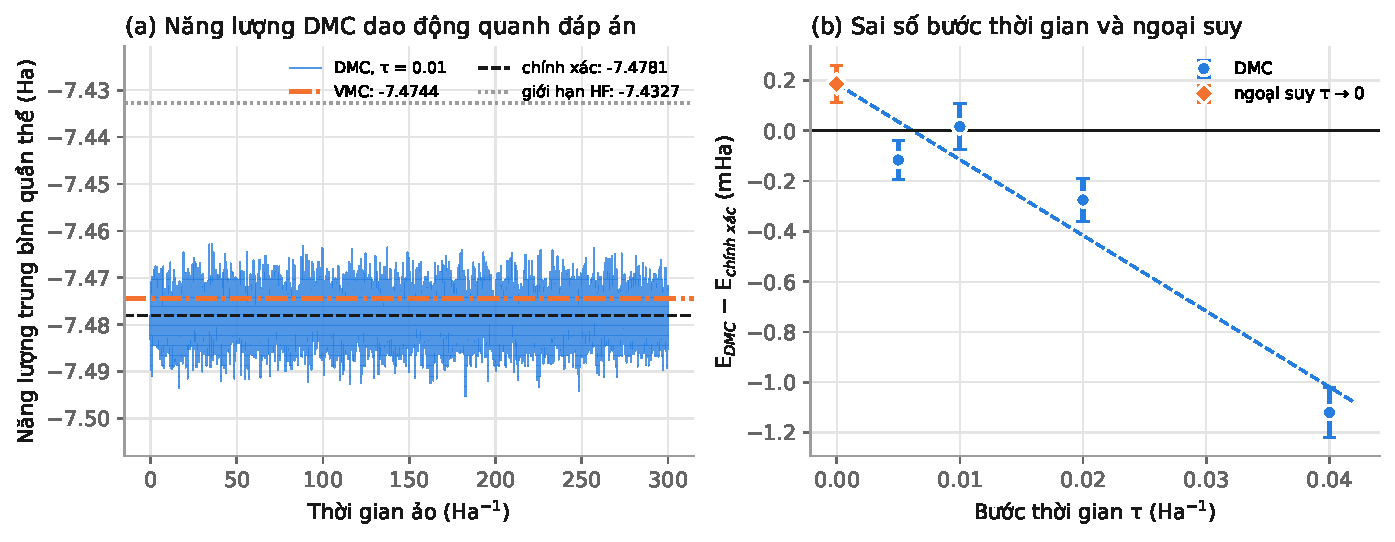
\includegraphics[width=\textwidth]{05_qmc_li.pdf}
\caption{(a) Năng lượng trung bình của quần thể walker DMC theo thời gian ảo ($\tau=0.01$): dao động thống kê quanh năng lượng chính xác (vạch đen), thấp hơn hẳn VMC (vạch cam) và giới hạn HF (vạch xám). (b) Năng lượng DMC theo bước thời gian $\tau$; đường nét đứt là ngoại suy tuyến tính về $\tau\to0$. (Script \code{05\_monte\_carlo\_luong\_tu.py})}
\label{fig:qmc}
\end{figure}

DMC ngoại suy về $\tau\to0$ cho $E=\Edmc\Ha$, tức lệch $\ErrDmc\mHa$ so với đáp án, với sai số thống kê $\pm\EdmcErr\mHa$. Ta thu được khoảng \PctDmc\% năng lượng tương quan bằng một chương trình vài trăm dòng, không cần tập cơ sở, với một hàm thử chỉ có 4 tham số. Đây là sức mạnh của QMC.

Cần nói thật một điều: độ lệch $\ErrDmc\mHa$ lớn hơn vài lần sai số thống kê ước tính, nên không thể coi hoàn toàn là nhiễu ngẫu nhiên. Có thể so với tài liệu: DMC chuyên nghiệp dùng \emph{đúng} mặt nút $r_1=r_2$ này (nút của hàm Hartree--Fock \cite{Bressanini2001}) cho $-7.47802(1)\Ha$, chỉ cao hơn đáp án $0.04\mHa$ \cite{Brown2007}. Vậy phần lớn độ lệch còn lại của ta \emph{không} do mặt nút, mà do cách cài đặt đơn giản: sai số bước thời gian chưa được khử hết (hình~\ref{fig:qmc}b cho thấy hai điểm có $\tau$ nhỏ nhất không thẳng hàng hoàn hảo), sai lệch nhỏ do cơ chế điều khiển số walker, và sai số thống kê bị ước tính hơi thấp vì các bước liên tiếp tương quan với nhau. Tách bạch các nguồn này là một bài tập hay cho người đọc. Dù vậy, sai số cỡ $0.2\mHa$ vẫn nhỏ hơn độ chính xác hóa học khoảng 8 lần.

\begin{table}[h]
\centering\small
\caption{So sánh với các kết quả QMC đã công bố cho Li.}
\label{tab:qmclit}
\begin{tabular}{@{}lrr@{}}
\toprule
Tính toán & $E$ (Ha) & \% tương quan \\
\midrule
VMC, Slater--Jastrow, 4 tham số (code đi kèm) & $\Evmc$ & \PctVmc \\
VMC, Slater--Jastrow chuyên nghiệp \cite{Brown2007} & $-7.47683(3)$ & 97.3 \\
VMC, nhiều định thức + Jastrow + backflow \cite{Seth2011} & $-7.478034(8)$ & 99.94 \\
DMC, nút $r_1=r_2$ (code đi kèm, $\tau\to0$) & $\Edmc$ & \PctDmc \\
DMC, nút Hartree--Fock \cite{Brown2007} & $-7.47802(1)$ & 99.91 \\
FermiNet, mạng nơ-ron (chương~\ref{ch:biengioi}) \cite{Pfau2020} & $-7.47798(1)$ & 99.82 \\
\midrule
Chính xác (Hylleraas) & $-7.478060$ & 100 \\
\bottomrule
\end{tabular}
\end{table}

Cũng cần nhớ: với Li, nút $r_1=r_2$ gần như chính xác; với các phân tử phức tạp hơn, sai số nút cố định thường cỡ vài mHa và là giới hạn chính của DMC \cite{Foulkes2001}.

\section{Ưu và nhược điểm}
\begin{itemize}
\item \textbf{Ưu:} chi phí tăng như $N^3$--$N^4$ theo số electron (cho mỗi mẫu); không cần tập cơ sở; dùng được hàm sóng chứa $r_{ij}$; song song hóa gần như hoàn hảo (mỗi walker độc lập), rất hợp với siêu máy tính; DMC thường chính xác ngang CCSD(T).
\item \textbf{Nhược:} kết quả luôn có sai số thống kê, muốn giảm 10 lần phải chạy lâu 100 lần; sai số nút cố định khó kiểm soát; tính lực (đạo hàm năng lượng theo vị trí hạt nhân) và các tính chất khác ngoài năng lượng khó hơn nhiều; cần nhiều kinh nghiệm để chọn hàm thử tốt.
\end{itemize}

\begin{ghinho}
\begin{itemize}
\item Monte Carlo tính tích phân nhiều chiều với sai số $\sim1/\sqrt M$, không phụ thuộc số chiều: một cách đi vòng bức tường hàm mũ.
\item VMC: năng lượng là trung bình của năng lượng cục bộ $E_L=\Hhat\Psi_T/\Psi_T$ trên các cấu hình lấy mẫu từ $|\Psi_T|^2$ bằng thuật toán Metropolis. Hàm Slater--Jastrow với 4 tham số thu \PctVmc\% tương quan của Li.
\item DMC: tiến hóa theo thời gian ảo để chiếu về trạng thái cơ bản. Fermion gây ra bài toán dấu; gần đúng nút cố định giải quyết bằng cách cấm walker vượt nút của hàm thử.
\item Điều kiện cusp là bắt buộc để DMC ổn định. Code tự viết đạt sai số $\ErrDmc\mHa$ so với đáp án 15 chữ số.
\end{itemize}
\end{ghinho}

\chapter{Biên giới: mạng nơ-ron, máy tính lượng tử, mạng tensor}
\label{ch:biengioi}

Chương này giới thiệu các hướng đang được nghiên cứu sôi động nhất (tính tới cuối năm 2026). Khác các chương trước, ở đây ta không tự chạy code, mà dựa vào kết quả đã công bố. Với các kết quả rất mới, tài liệu ghi rõ khi nào đó chỉ là bản thảo chưa qua bình duyệt \en{preprint}.

\section{Hàm sóng mạng nơ-ron}

\begin{eli5}[một hàm biến hình có hàng triệu núm vặn]
Mạng nơ-ron là một cỗ máy nhận vào vị trí của mọi electron và trả ra một con số: giá trị hàm sóng. Nó có hàng trăm nghìn tới hàng triệu ``núm vặn'' (tham số), nên có thể ``nặn'' thành gần như mọi hình dạng. Điều thú vị: ta \emph{không cần dữ liệu huấn luyện}. Chính phương trình Schrödinger là ``thầy giáo'': ta vặn núm sao cho năng lượng VMC (chương~\ref{ch:qmc}) thấp nhất. Nguyên lý biến phân đảm bảo năng lượng thấp hơn nghĩa là hàm sóng tốt hơn.

\emph{Chỗ ví dụ ``gãy'':} linh hoạt không có nghĩa là chắc chắn đúng. Huấn luyện tốn hàng trăm tới hàng chục nghìn giờ GPU, có yếu tố ngẫu nhiên, và có thể bị kẹt.
\end{eli5}

Ý tưởng dùng mạng nơ-ron làm hàm sóng xuất hiện năm 2017 với các mô hình spin \cite{Carleo2017}. Năm 2019--2020, hai nhóm độc lập áp dụng nó cho electron trong không gian thực: FermiNet của DeepMind \cite{Pfau2020} và PauliNet của nhóm Berlin \cite{Hermann2020}.

\begin{congthuc}[ý tưởng của FermiNet]
Hàm sóng vẫn có dạng định thức (để đảm bảo phản đối xứng), nhưng các ``orbital'' được thay bằng đầu ra của mạng nơ-ron:
\[
\Psi(\vr_1,\ldots,\vr_N)=\sum_{k}\omega_k\,\det\big[\phi^{k}_i(\vr_j;\{\vr_{/j}\})\big]_{\uparrow}\,\det\big[\phi^{k}_i(\vr_j;\{\vr_{/j}\})\big]_{\downarrow} .
\]
\begin{itemize}
\item Khác orbital thông thường $\phi_i(\vr_j)$ chỉ phụ thuộc vị trí electron $j$, ``orbital tổng quát'' $\phi_i(\vr_j;\{\vr_{/j}\})$ phụ thuộc vào electron $j$ \emph{và} vào mọi electron khác, nhưng đối xứng theo các electron khác đó. Nhờ vậy đổi chỗ hai electron cùng spin vẫn là đổi hai cột của ma trận, và định thức vẫn đổi dấu: phản đối xứng được đảm bảo chính xác.
\item Đầu vào của mạng là vị trí electron so với hạt nhân và khoảng cách giữa các electron ($|\vr_i-\vr_j|$). Nhờ có khoảng cách này, mạng ``học'' được cả tương quan lẫn điều kiện cusp.
\item Mạng được huấn luyện bằng cách cực tiểu hóa năng lượng VMC, với mẫu lấy bằng thuật toán Metropolis đúng như chương~\ref{ch:qmc}.
\item Chi phí một bước tối ưu tăng khoảng $N^4$ theo số electron, với hệ số rất lớn \cite{Pfau2020}.
\end{itemize}
\end{congthuc}

\begin{table}[h]
\centering\small
\caption{FermiNet (2020) cho các nguyên tử chu kỳ 2: sai số so với năng lượng chính xác và phần trăm năng lượng tương quan thu được \cite{Pfau2020}. Mọi nguyên tử đều đạt độ chính xác hóa học ($1.6\mHa$).}
\label{tab:ferminet}
\begin{tabular}{@{}lrrrr@{}}
\toprule
Nguyên tử & FermiNet (Ha) & Chính xác (Ha) & Sai số (mHa) & \% tương quan \\
\midrule
Li & $-7.47798(1)$ & $-7.47806$ & $+0.08$ & 99.82 \\
Be & $-14.66733(3)$ & $-14.66736$ & $+0.03$ & 99.97 \\
B & $-24.65370(3)$ & $-24.65391$ & $+0.21$ & 99.83 \\
C & $-37.84471(5)$ & $-37.8450$ & $+0.29$ & 99.81 \\
N & $-54.58882(6)$ & $-54.5892$ & $+0.38$ & 99.80 \\
O & $-75.06655(7)$ & $-75.0673$ & $+0.75$ & 99.70 \\
Ne & $-128.9366(1)$ & $-128.9376$ & $+1.0$ & 99.74 \\
\bottomrule
\end{tabular}
\end{table}

\paragraph{Các bước tiến 2020--2026.}
\begin{itemize}
\item \textbf{PauliNet} \cite{Hermann2020} giữ ``khung vật lý'' Slater--Jastrow (orbital HF làm nền, cusp cài sẵn) và dùng mạng nơ-ron cho phần tương quan, nên cần ít tài nguyên hơn.
\item \textbf{Psiformer} \cite{vonGlehn2023} dùng cơ chế \emph{self-attention} của kiến trúc Transformer (cùng họ với các mô hình ngôn ngữ lớn). Với benzen, Psiformer cho năng lượng thấp hơn kết quả DMC tốt nhất đã công bố.
\item \textbf{Forward Laplacian / LapNet} \cite{LiLapNet2024}: tính laplacian (cần cho năng lượng cục bộ) trong một lượt truyền xuôi duy nhất, tăng tốc hơn 10 lần.
\item \textbf{Trạng thái kích thích} \cite{Pfau2024}: với Li, năng lượng kích thích 2s $\to$ 2p tính được là $0.06790\Ha$, so với thực nghiệm $0.067907\Ha$, sai dưới $0.005\mHa$.
\item \textbf{Mô hình nền tảng} \cite{Scherbela2024}: huấn luyện trước một mạng trên nhiều phân tử rồi chỉ cần tinh chỉnh cho phân tử mới, giảm mạnh chi phí cho mỗi phân tử.
\end{itemize}

\paragraph{Hạn chế (nói thẳng).}
Chi phí GPU rất lớn: hàng nghìn giờ GPU cho phân tử cỡ benzen \cite{vonGlehn2023}. Phần trăm tương quan thu được giảm dần khi hệ lớn lên. Tối ưu hóa mang tính ngẫu nhiên, kết quả dao động giữa các lần chạy, và không có thanh sai số hệ thống chặt chẽ. Với Li, các phương pháp này đã ``bão hòa'' ở mức sai số micro-hartree: Li trở thành bài kiểm tra chuẩn chứ không còn là mục tiêu nghiên cứu.

\section{Máy tính lượng tử}

\begin{eli5}[muốn mô phỏng dàn nhạc, hãy dùng một dàn nhạc]
Ghi lại mọi sóng âm của một bản giao hưởng lên giấy thì vô cùng tốn, nhưng một dàn nhạc thật ``tự nhiên'' tạo ra nó. Tương tự, trạng thái của $n$ qubit cần $2^n$ số phức để lưu trên máy tính cổ điển, còn máy tính lượng tử ``chứa'' nó trong $n$ qubit. Năm 1982, Feynman đề xuất: hãy dùng một hệ lượng tử điều khiển được để mô phỏng hệ lượng tử khác \cite{Feynman1982}. Đây là cách ``đi xuyên'' bức tường hàm mũ thay vì đi vòng.

\emph{Chỗ ví dụ ``gãy'':} ta không ``đọc'' được cả $2^n$ biên độ; mỗi phép đo chỉ cho một kết quả ngẫu nhiên, nên phải lặp hàng nghìn tới hàng triệu lần. Qubit hiện nay rất ``ồn'', giống một dàn nhạc mà nhạc cụ lạc dây sau vài giây.
\end{eli5}

\begin{congthuc}[từ electron sang qubit]
Trong ngôn ngữ lượng tử hóa lần hai, mỗi spin-orbital $j$ hoặc có electron ($n_j=1$) hoặc trống ($n_j=0$), giống một qubit. Phép ánh xạ \textbf{Jordan--Wigner} \cite{JordanWigner1928} viết toán tử ``đặt electron vào orbital $j$'' thành
\[
a_j^\dagger=Z_0\otimes Z_1\otimes\cdots\otimes Z_{j-1}\otimes\frac{X_j-iY_j}{2},
\]
với $X,Y,Z$ là các ma trận Pauli tác động lên từng qubit. Chuỗi $Z$ phía trước đảm bảo dấu phản đối xứng của fermion. Hamiltonian trở thành tổng của các ``chuỗi Pauli'': $\Hhat=\sum_kc_kP_k$. Số qubit bằng số spin-orbital, tức gấp đôi số hàm cơ sở.
\end{congthuc}

\begin{table}[h]
\centering\small
\caption{Li cần bao nhiêu qubit? (ánh xạ Jordan--Wigner, mỗi spin-orbital một qubit). Số liệu do subagent nghiên cứu tự tính bằng PySCF và OpenFermion; cột cuối là sai số của nghiệm \emph{chính xác} trong tập cơ sở đó, tức kết quả tốt nhất mà một máy tính lượng tử hoàn hảo có thể cho.}
\label{tab:qubit}
\begin{tabular}{@{}lrrr@{}}
\toprule
Tập cơ sở & Số qubit & Số chuỗi Pauli & Sai số của Full CI (mHa) \\
\midrule
STO-3G & 10 & 156 & $+162$ \\
6-31G & 18 & 3\,388 & $+46.5$ \\
cc-pCVDZ & 36 & --- & $+12.0$ \\
cc-pCVTZ & 86 & --- & $+3.8$ \\
\bottomrule
\end{tabular}
\end{table}

Bảng~\ref{tab:qubit} cho một bài học trung thực: một máy tính lượng tử ``giải đúng'' Li trong tập STO-3G (10 qubit) vẫn sai khoảng 100\,kcal/mol so với thực tế, vì tập cơ sở quá nhỏ. Muốn sai số vài mHa cần khoảng 86 qubit \emph{hoàn hảo}, trong khi máy tính cổ điển giải Full CI của chính bài toán đó trong vài phút (chương~\ref{ch:sauhf}). Li là bài tập sư phạm, không phải ứng viên cho ``lợi thế lượng tử''.

\subsection{VQE: đầu bếp lượng tử và người nếm cổ điển}

\begin{eli5}[đầu bếp và người nếm]
Máy lượng tử làm ``đầu bếp'': nấu một trạng thái thử theo công thức có vài núm vặn. Máy cổ điển làm ``người nếm'': đo năng lượng rồi bảo đầu bếp vặn núm. Lặp lại tới khi món ăn (năng lượng) ngon nhất. Đây chính là nguyên lý biến phân, chỉ khác là hàm thử được ``nấu'' trên phần cứng lượng tử.

\emph{Chỗ ví dụ ``gãy'':} mỗi lần nếm phải đo hàng triệu lần vì kết quả lượng tử là ngẫu nhiên; mặt năng lượng có thể phẳng lì (``barren plateau'') khiến không biết vặn núm theo hướng nào \cite{McClean2018}; và nhiễu phần cứng làm món ăn sai vị.
\end{eli5}

\textbf{VQE} \en{Variational Quantum Eigensolver} được đề xuất năm 2014 \cite{Peruzzo2014}: $E(\boldsymbol\theta)=\langle\psi(\boldsymbol\theta)|\Hhat|\psi(\boldsymbol\theta)\rangle\ge E_0$. Các mốc thực nghiệm: HeH$^+$ trên chip quang tử 2 qubit (2014) \cite{Peruzzo2014}; H$_2$, LiH, BeH$_2$ trên 2--6 qubit của IBM (2017) \cite{Kandala2017}; Hartree--Fock cho chuỗi H$_{12}$ trên bộ xử lý Sycamore của Google (2020) \cite{Google2020}. Lưu ý: Hartree--Fock là bài toán \emph{dễ} với máy cổ điển; thí nghiệm năm 2020 là để kiểm định phần cứng.

\subsection{Ước lượng pha lượng tử và máy tính chịu lỗi}
Về lâu dài, thuật toán \textbf{ước lượng pha lượng tử} (QPE) có thể cho năng lượng chính xác trong tập cơ sở, nhưng cần mạch rất sâu, tức là cần máy tính lượng tử \emph{chịu lỗi} \en{fault-tolerant} với hàng nghìn qubit logic được sửa lỗi. Bài toán ``biểu tượng'' là cụm FeMoco của enzyme nitrogenase (cố định nitơ trong tự nhiên). Ước tính năm 2021 cần khoảng 4 triệu qubit vật lý chạy dưới 4 ngày \cite{LeeTHC2021}. Phần cứng đang tiến bộ thật: năm 2025, Google chứng minh bộ nhớ lượng tử sửa lỗi hoạt động dưới ngưỡng \cite{Willow2025}; năm 2026, Quantinuum chạy trọn QPE trên qubit đã mã hóa sửa lỗi cho phân tử H$_2$, nhưng sai số thống kê ($13\mHa$) vẫn lớn hơn độ chính xác hóa học \cite{Yamamoto2026}.

\subsection{Đánh giá thẳng thắn}
Một nhóm tác giả gồm cả chuyên gia máy tính lượng tử lẫn hóa lượng tử cổ điển đã xem xét kỹ giả thuyết ``máy tính lượng tử sẽ nhanh hơn theo hàm mũ'' cho bài toán năng lượng trạng thái cơ bản, và kết luận \cite{Lee2023}: \emph{``evidence for such an exponential advantage across chemical space has yet to be found''} (bằng chứng cho lợi thế theo hàm mũ trên toàn bộ không gian hóa học vẫn chưa được tìm thấy). Lý do: chính những tính chất làm cho trạng thái dễ chuẩn bị trên máy lượng tử cũng làm cho các phương pháp cổ điển (DMRG, Coupled Cluster) hoạt động tốt. Tăng tốc theo đa thức vẫn có thể có. Một bản thảo năm 2026 (chưa bình duyệt) còn cho thấy mô hình FeMoco 76 orbital, vốn dùng trong phần lớn các ước tính tài nguyên lượng tử, có thể được giải tới gần độ chính xác hóa học bằng máy tính cổ điển \cite{Zhai2026}. Tóm lại, tính tới cuối 2026: \textbf{chưa có tính toán lượng tử nào cho năng lượng trạng thái cơ bản có ý nghĩa hóa học vượt khả năng của máy tính cổ điển}. Triển vọng dài hạn nằm ở máy chịu lỗi, hệ tương quan mạnh lớn và bài toán động lực học, và vẫn còn tranh luận.

\section{Mạng tensor và DMRG}

\begin{eli5}[nén ảnh và hàng người nắm tay]
Một bức ảnh khổng lồ có thể nén vì phần lớn thông tin nằm trong vài ``mẫu'' chính. DMRG nén hàm sóng theo cách tương tự: xếp các orbital thành một hàng, mỗi orbital chỉ ``nắm tay'' (trao đổi thông tin) với hàng xóm qua một sợi dây có ``băng thông'' giới hạn $M$. Nếu tương quan chủ yếu xảy ra giữa các orbital gần nhau trong hàng, vài nghìn kênh là đủ thay cho con số thiên văn.

\emph{Chỗ ví dụ ``gãy'':} nếu hệ có tương quan tầm xa hoặc có cấu trúc 2, 3 chiều, ``băng thông'' cần tăng theo hàm mũ.
\end{eli5}

\begin{congthuc}[trạng thái tích ma trận]
DMRG \cite{White1992} biểu diễn hàm sóng dưới dạng \textbf{trạng thái tích ma trận} \en{matrix product state, MPS}:
\[
|\Psi\rangle=\sum_{n_1,\ldots,n_k}A^{[1]n_1}A^{[2]n_2}\cdots A^{[k]n_k}\,|n_1n_2\cdots n_k\rangle ,
\]
trong đó $n_i\in\{0,\uparrow,\downarrow,\uparrow\!\downarrow\}$ là trạng thái chiếm của orbital $i$, và mỗi $A^{[i]n_i}$ là ma trận $M\times M$. Số tham số khoảng $4kM^2$ thay vì $4^k$. Với các hệ một chiều có khe năng lượng, ``luật diện tích'' của độ vướng víu đảm bảo $M$ hữu hạn là đủ \cite{ChanSharma2011}.
\end{congthuc}

DMRG mạnh nhất ở nơi các phương pháp khác yếu: \textbf{tương quan tĩnh mạnh} với hàng chục tới hơn 100 orbital hoạt động, như cụm Mn$_4$CaO$_5$ trong quang hợp \cite{Kurashige2013} hay phân tử Cr$_2$ nổi tiếng khó \cite{Larsson2022}. Ngược lại, DMRG \emph{không cần thiết} cho Li: tương quan của Li là tương quan \emph{động} của cặp lõi 1s$^2$, trải trên rất nhiều orbital ảo ít chiếm, đúng loại mà DMRG xử lý kém hiệu quả.

\section{``Full CI mà không cần liệt kê hết''}
Hai họ phương pháp khác tấn công trực tiếp bức tường tổ hợp của Full CI:
\begin{itemize}
\item \textbf{FCIQMC} \cite{Booth2009}: một ``đàn kiến'' walker mang dấu $+$ hoặc $-$ đi lại giữa các định thức Slater, sinh con, chết, và triệt tiêu khi gặp walker trái dấu. Khi đủ đông, phân bố walker cho đúng hàm sóng Full CI mà không cần biết trước mặt nút. Bài toán dấu vẫn còn, nhưng ở dạng nhẹ hơn: cần vượt qua một ``số walker tới hạn''.
\item \textbf{Selected CI} (CIPSI, HCI, SHCI) \cite{Holmes2016}: trong hàng tỉ tỉ định thức, chỉ vài triệu thực sự quan trọng. Ta ``tuyển chọn'' dần những định thức tương tác mạnh nhất với hàm sóng hiện tại, rồi bổ sung phần còn lại bằng lý thuyết nhiễu loạn. HCI đã đạt độ chính xác Full CI (sai số dưới $1\mHa$) cho phân tử Cr$_2$ trong một không gian $2\times10^{22}$ định thức.
\end{itemize}
Một thử nghiệm ``mù'' năm 2020 \cite{Eriksen2020} cho nhiều nhóm dùng các phương pháp gần chính xác khác nhau (DMRG, FCIQMC, SHCI, Coupled Cluster bậc cao\ldots) cùng tính năng lượng Full CI của benzen trong một tập cơ sở nhỏ. Các kết quả lệch nhau khoảng $1\mHa$. Ngay cả ``gần chính xác'' vẫn khó ở 30 electron.

\begin{ghinho}
\begin{itemize}
\item Hàm sóng mạng nơ-ron (FermiNet, PauliNet, Psiformer) là VMC với hàm thử cực kỳ linh hoạt. Kết quả rất chính xác (Li sai $0.08\mHa$ năm 2020, micro-hartree năm 2024), nhưng tốn nhiều GPU.
\item Máy tính lượng tử ``đi xuyên'' bức tường hàm mũ về nguyên tắc. Thực tế tới 2026: phần cứng tiến bộ nhanh, nhưng chưa có lợi thế cho năng lượng trạng thái cơ bản có ý nghĩa hóa học; lợi thế theo hàm mũ vẫn chưa có bằng chứng.
\item DMRG nén hàm sóng thành tích các ma trận; mạnh cho tương quan tĩnh và hệ dạng chuỗi, không cần cho Li.
\item FCIQMC và selected CI mở rộng Full CI tới những không gian khổng lồ bằng cách chỉ ghé thăm các định thức quan trọng.
\end{itemize}
\end{ghinho}

\chapter{Tổng kết: bức tranh toàn cảnh}
\label{ch:tongket}

\section{Một biểu đồ cho tất cả}

Hình~\ref{fig:tongket} đặt mọi phương pháp đã chạy trong tài liệu lên cùng một thước đo: sai số năng lượng của nguyên tử Li so với đáp án 15 chữ số. Trục hoành dùng thang log, mỗi vạch chia là một bậc độ chính xác (gấp 10 lần).

\begin{figure}[h]
\centering
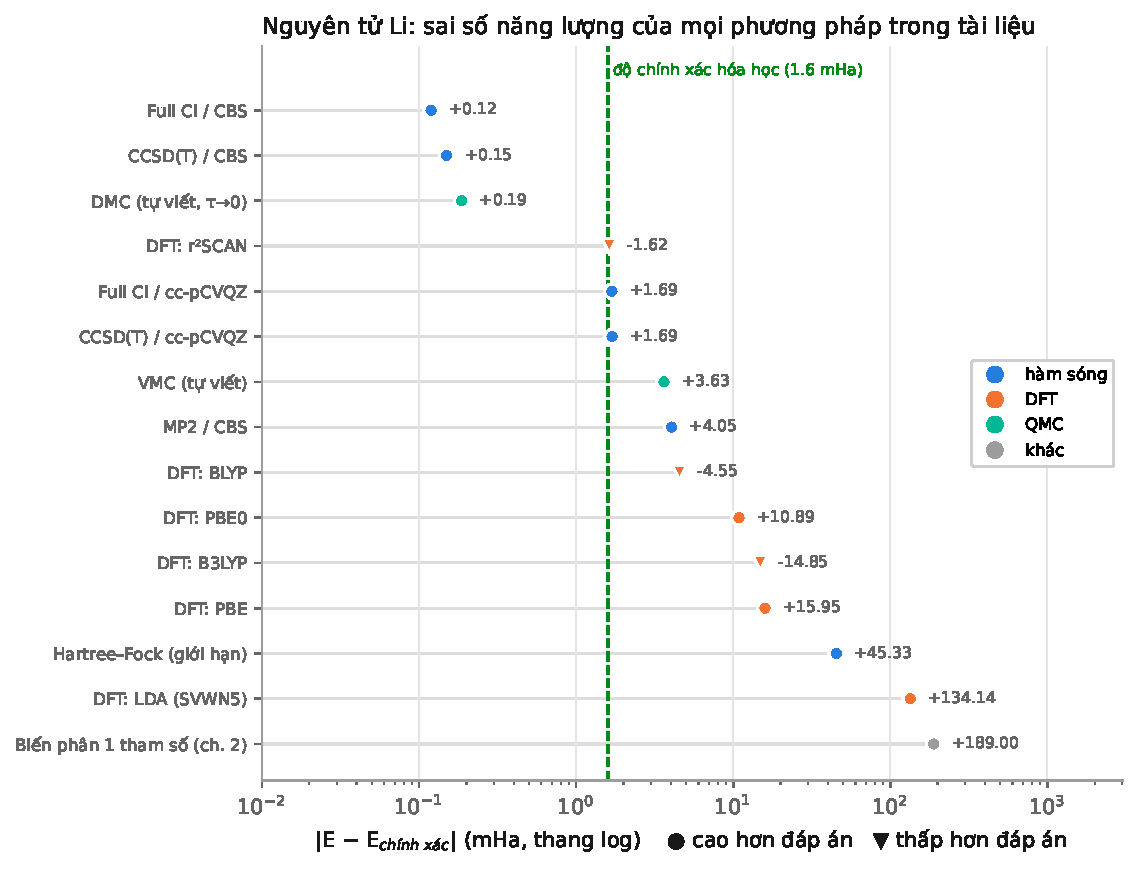
\includegraphics[width=\textwidth]{06_tong_ket.pdf}
\caption{Sai số năng lượng của Li với mọi phương pháp trong tài liệu, sắp xếp từ chính xác nhất (dưới) tới kém nhất (trên). Màu theo họ phương pháp: xanh dương là hàm sóng, cam là DFT, xanh ngọc là Monte Carlo lượng tử tự viết. Hình tròn: cao hơn đáp án; tam giác: thấp hơn đáp án (chỉ xảy ra với DFT và với sai số thống kê của DMC). Vạch xanh lá: độ chính xác hóa học. (Script \code{06\_tong\_hop.py})}
\label{fig:tongket}
\end{figure}

\section{Bảng so sánh}

\begin{table}[h]
\centering\small
\caption{So sánh các phương pháp. Cột ``Li'' là sai số năng lượng toàn phần tính bằng code đi kèm (mHa).}
\label{tab:tongket}
\begin{tabularx}{\textwidth}{@{}l>{\raggedright\arraybackslash}X>{\raggedright\arraybackslash}p{1.6cm}r>{\raggedright\arraybackslash}X@{}}
\toprule
Phương pháp & Xấp xỉ điều gì & Chi phí & Li & Dùng khi nào \\
\midrule
Hartree--Fock & Một định thức; electron khác spin không né nhau & $N^4$ & $+45.3$ & Điểm xuất phát cho mọi phương pháp hàm sóng \\
MP2 & Tương quan như nhiễu loạn bậc 2 & $N^5$ & $\ErrMPtwoCBS$ & Ước lượng nhanh tương quan (CBS) \\
CCSD(T) & Kích thích đơn, đôi (lặp) + ba (nhiễu loạn) & $N^7$ & $\ErrCCSDTCBS$ & Chuẩn vàng cho phân tử nhỏ, vừa, đơn tham chiếu (CBS) \\
Full CI & Không xấp xỉ, chỉ giới hạn bởi tập cơ sở & $e^N$ & $\ErrFciCBS$ & Hệ rất nhỏ; làm chuẩn để kiểm tra (CBS) \\
LDA & Mỗi điểm như khí electron đồng nhất & $N^3$ & $\ErrLDA$ & Chủ yếu cho chất rắn, lịch sử \\
PBE & Thêm độ dốc mật độ & $N^3$ & $\ErrPBE$ & Vật liệu, chất rắn, hệ lớn \\
B3LYP & Thêm 20\% trao đổi chính xác & $N^4$ & $\ErrBthreeLYP$ & Hóa học phân tử thường ngày \\
VMC & Dạng hàm thử (Slater--Jastrow) & $N^3$--$N^4$ & $\ErrVmc$ & Kiểm tra, tối ưu hàm thử \\
DMC & Nút của hàm thử & $N^3$--$N^4$ & $\ErrDmc$ & Độ chính xác cao, hệ lớn, song song tốt \\
Mạng nơ-ron & Kiến trúc và quá trình huấn luyện & $N^4$ & --- & Nghiên cứu: hệ nhỏ, vừa, cực chính xác \\
Máy lượng tử & Số qubit, nhiễu, độ sâu mạch & --- & --- & Nghiên cứu; tương lai cho tương quan mạnh \\
\bottomrule
\end{tabularx}
\end{table}

\section{Bốn chiến lược vượt bức tường hàm mũ}

Nhìn lại toàn bộ tài liệu, mọi phương pháp đều là một cách ``lách'' bức tường hàm mũ của chương~\ref{ch:baitoan}. Có bốn chiến lược chính:

\begin{enumerate}
\item \textbf{Thu hẹp dạng hàm sóng.} Không cho hàm sóng tự do, mà chỉ tìm trong một ``lớp'' hàm có cấu trúc: một định thức (HF), định thức nhân $e^{\hat T}$ cắt ngắn (CC), định thức nhân thừa số Jastrow (VMC). Số tham số chỉ tăng theo đa thức. Cái giá: sai số do chọn lớp hàm.
\item \textbf{Đổi biến.} Thay hàm sóng $3N$ chiều bằng mật độ 3 chiều (DFT). Bài toán trở nên rẻ, nhưng mọi khó khăn dồn vào phiếm hàm $E_{xc}$ chưa biết.
\item \textbf{Lấy mẫu ngẫu nhiên.} Không lưu hàm sóng, chỉ lấy mẫu nó (QMC). Sai số thống kê giảm như $1/\sqrt M$ bất kể số chiều. Cái giá: bài toán dấu của fermion, xử lý gần đúng bằng nút cố định.
\item \textbf{Biểu diễn mới.} Dùng các cấu trúc dữ liệu có khả năng nén thông tin tốt hơn: mạng nơ-ron, mạng tensor, hay trạng thái của chính một hệ lượng tử khác (máy tính lượng tử). Chương~\ref{ch:biengioi} trình bày các hướng này.
\end{enumerate}

\begin{eli5}[bốn cách xếp hành lý]
Bạn phải mang theo một ``tủ quần áo'' khổng lồ (hàm sóng chính xác) mà không vali nào chứa nổi. Cách 1: chỉ mang những bộ đồ theo vài kiểu cố định (thu hẹp dạng hàm). Cách 2: chỉ mang tấm ảnh chụp tủ quần áo, rồi dùng ``công thức'' để suy ra mọi thứ khác (đổi biến, DFT). Cách 3: mỗi ngày bốc ngẫu nhiên vài bộ, đủ để biết ``trung bình'' bạn mặc gì (lấy mẫu). Cách 4: phát minh ra một loại vali hút chân không nén được quần áo (biểu diễn mới).
\end{eli5}

\section{Điều gì đã giải quyết, điều gì còn mở?}

\paragraph{Đã giải quyết khá tốt.}
Nguyên tử và phân tử nhỏ mà hàm sóng có một cấu hình chiếm ưu thế, như Li trong tài liệu này: CCSD(T) ngoại suy về tập cơ sở vô hạn và DMC đều đạt độ chính xác hóa học. Với hệ lớn hơn (hàng trăm, hàng nghìn nguyên tử), DFT cho kết quả ``đủ dùng'' với chi phí chấp nhận được.

\paragraph{Còn mở.}
\begin{itemize}
\item \textbf{Tương quan mạnh}: khi nhiều cấu hình quan trọng ngang nhau (kim loại chuyển tiếp, liên kết bị kéo giãn, chất siêu dẫn nhiệt độ cao, vật liệu từ), cả CCSD(T) lẫn DFT thông thường đều thất bại, còn các phương pháp đa tham chiếu lại tăng chi phí theo hàm mũ.
\item \textbf{Hệ lớn với độ chính xác cao}: đưa độ chính xác cỡ CCSD(T) hay DMC tới protein, bề mặt xúc tác, vật liệu thực.
\item \textbf{Một phiếm hàm DFT ``tốt cho mọi thứ''}: chưa có, và không có con đường cải thiện có hệ thống.
\item \textbf{Bài toán dấu}: chưa có cách giải tổng quát, và có lý do lý thuyết (NP-khó) để tin rằng sẽ không có \cite{TroyerWiese2005}.
\end{itemize}

\section{Lời kết}

Ta bắt đầu từ câu nói của Dirac năm 1929: các định luật đã biết hết, chỉ có phương trình là quá phức tạp để giải. Gần một thế kỷ sau, điều đó vẫn đúng, nhưng ta đã đi được một chặng rất dài. Với nguyên tử Li, một chương trình Hartree--Fock 30 dòng cho 99.4\% năng lượng. Full CI trên máy tính xách tay cùng phép ngoại suy thông minh đạt sai số $\ErrFciCBS\mHa$. Một chương trình Monte Carlo vài trăm dòng tự viết đạt độ chính xác tương đương mà không cần tập cơ sở nào. Mỗi phương pháp là một ý tưởng vật lý đẹp: trường trung bình, phản đối xứng, lãi kép, mật độ thay cho hàm sóng, mực loang trong thời gian ảo.

Nếu bạn muốn đi tiếp, Phụ lục~\ref{pl:lotrinh} có lộ trình chi tiết, Phụ lục~\ref{pl:tailieu} có tài liệu nên đọc, và thư mục \code{code/} là nơi tốt nhất để bắt đầu: sửa một tham số, chạy lại, và xem điều gì thay đổi.


\appendix
\renewcommand{\chaptertitlename}{Phụ lục}
\chapter{Lộ trình tự học}
\label{pl:lotrinh}

Phụ lục này dành cho bạn nếu muốn đi từ ``đọc hiểu tài liệu này'' tới ``tự tính toán và đọc được bài báo chuyên ngành''. Lộ trình gồm 9 giai đoạn, giả định bạn học khoảng 10--12 giờ mỗi tuần. Toàn bộ giai đoạn 1--8 mất khoảng \textbf{20--36 tháng}, tương đương 2--3 năm đại học cộng một năm cao học. Học chậm hơn dự kiến là hoàn toàn bình thường. Mã [B\ldots] chỉ tới tài liệu ở Phụ lục~\ref{pl:tailieu}.

\section*{Nguyên tắc}
\begin{itemize}
\item \textbf{Học bằng cách tính toán.} Giai đoạn nào cũng có bài tập lập trình. Dùng nguyên tử Li làm ``dự án xuyên suốt'': mỗi giai đoạn, bạn tiến gần thêm một bước tới con số $-7.478\Ha$.
\item \textbf{Ưu tiên tài liệu miễn phí và dễ đọc}, sau đó tới sách chuẩn (mượn thư viện), cuối cùng là tài liệu chuyên sâu chỉ để tra cứu.
\item \textbf{Tiếng Anh} là ngôn ngữ của hầu hết tài liệu tốt. Dùng bảng thuật ngữ (Phụ lục~\ref{pl:thuatngu}), ghi chép bằng tiếng Việt, bật phụ đề khi xem video.
\item \textbf{Kỹ thuật học}: tự giảng lại bằng lời của mình (kỹ thuật Feynman), tự kiểm tra mà không nhìn sách, làm bài tập trước khi xem lời giải.
\item \textbf{Ba lối đi}: \emph{Lối A}, người dùng tính toán (chỉ cần chạy PySCF/Psi4 cho nghiên cứu): khoảng 6--9 tháng, đi G1 (rút gọn), G2, G3 (rút gọn), G6, G7. \emph{Lối B}, hiểu sâu lý thuyết: đi đủ G1 tới G8. \emph{Lối C}, phát triển phương pháp mới: Lối B rồi G9 và đọc bài báo gốc.
\end{itemize}

\section*{Tổng quan các giai đoạn}
\begin{center}
\small
\begin{tabularx}{\textwidth}{@{}l>{\raggedright\arraybackslash}p{3.3cm}l>{\raggedright\arraybackslash}X@{}}
\toprule
& Nội dung & Thời gian & Mốc kiểm tra \\
\midrule
G1 & Toán: giải tích, đại số tuyến tính, phương trình vi phân, xác suất & 3--6 tháng & Chéo hóa ma trận đối xứng; tách biến; giải thích sai số $\sigma/\sqrt M$ \\
G2 & Python khoa học (song song suốt lộ trình) & 1--2 tháng & Giải phương trình Schrödinger 1D bằng sai phân hữu hạn \\
G3 & Cơ học lượng tử một hạt & 4--6 tháng & Giải hydro và Li$^{2+}$; biến phân cho He \\
G4 & Nguyên tử nhiều electron, spin, hạt đồng nhất & 6--10 tuần & Viết định thức Slater 3$\times$3 cho Li; hiểu $J$, $K$ \\
G5 & Lượng tử hóa lần thứ hai & 4--6 tuần & Viết $\Hhat$ bằng toán tử sinh/hủy; đếm số định thức \\
G6 & Hartree--Fock và sau HF & 3--5 tháng & Tự viết RHF, MP2, CCSD; tính Li từ HF tới FCI \\
G7 & Lý thuyết phiếm hàm mật độ & 2--3 tháng & Năng lượng ion hóa Li bằng LDA/PBE/B3LYP \\
G8 & Monte Carlo lượng tử & 2--3 tháng & Tự viết VMC cho He; VMC/DMC cho Li \\
G9 & Biên giới (chọn một nhánh): mạng nơ-ron / máy tính lượng tử / DMRG & 3--6 tháng mỗi nhánh & Chạy FermiNet cho Li; VQE cho H$_2$; DMRG \\
\bottomrule
\end{tabularx}
\end{center}

Thứ tự phụ thuộc: G1 $\to$ G3 $\to$ G4 $\to$ G5 $\to$ G6, rồi tách thành G7 (DFT) và G8 (QMC, cần thêm xác suất ở G1). G9a (mạng nơ-ron) cần G8 và học máy cơ bản; G9b (máy tính lượng tử) cần G5 và G6; G9c (DMRG) cần G5 và phân tích SVD ở G1. G2 (Python) đi song song suốt lộ trình.

\section*{Chi tiết từng giai đoạn}

\paragraph{G1 --- Toán nền tảng (3--6 tháng).}
\emph{Nội dung:} giải tích một và nhiều biến (tích phân bội, tọa độ cầu, tích phân Gauss $\int e^{-ax^2}dx=\sqrt{\pi/a}$); số phức; \textbf{đại số tuyến tính} (quan trọng nhất: trị riêng, ma trận Hermite, bài toán trị riêng tổng quát $\mathbf{Hc}=\varepsilon\mathbf{Sc}$, phân tích SVD); phương trình vi phân và bài toán trị riêng; xác suất (kỳ vọng, phương sai, định lý giới hạn trung tâm). \emph{Tài liệu:} 3Blue1Brown [B33] trước tiên, rồi MIT 18.06 [B28], MIT 18.01SC/18.02SC/18.03 [B29,B31,B32], Harvard Stat 110 [B36]. \emph{Sẵn sàng khi:} bạn chéo hóa được ma trận đối xứng 3$\times$3 bằng tay và bằng máy, và giải thích được vì sao trung bình của $M$ mẫu ngẫu nhiên có sai số cỡ $\sigma/\sqrt M$.

\paragraph{G2 --- Python khoa học (song song).}
Python, NumPy (đặc biệt \code{einsum}, rất quan trọng khi làm việc với tích phân hai electron), SciPy, Matplotlib, Jupyter, git. \emph{Tài liệu:} Scientific Python Lectures [B52], NumPy cho người mới [B53]. \emph{Bài tập:} giải phương trình Schrödinger cho hạt trong hộp và dao động tử điều hòa bằng sai phân hữu hạn, so với nghiệm giải tích.

\paragraph{G3 --- Cơ học lượng tử một hạt (4--6 tháng).}
Hàm sóng, toán tử, phương trình Schrödinger 1D và 3D, mômen động lượng, nguyên tử hydro, nguyên lý biến phân, lý thuyết nhiễu loạn. \emph{Tài liệu:} MIT 8.04/8.05 [B21,B23] hoặc ghi chú miễn phí của David Tong [B19]; sách Griffiths [B1] chương 1--4, 7--8; Feynman tập III [B20] để có trực giác. \emph{Sẵn sàng khi:} bạn tự suy ra $E_n=-Z^2/(2n^2)$ và làm lại phép tính biến phân cho He ở chương~\ref{ch:hatdongnhat} mà không nhìn sách.

\paragraph{G4 --- Nhiều electron, spin, hạt đồng nhất (6--10 tuần).}
Spin, hạt đồng nhất, phản đối xứng, định thức Slater, quy tắc Slater--Condon, tích phân $J$ và $K$, cấu hình electron và ký hiệu số hạng. \emph{Tài liệu:} Griffiths chương 5 [B1]; MIT 5.61 bài 22--23 [B25]; video TMP Chem chương 9 [B37]. \emph{Sẵn sàng khi:} bạn tự suy ra công thức $E(\zeta)$ của Li ở mục~\ref{sec:bienphan}.

\paragraph{G5 --- Lượng tử hóa lần thứ hai (4--6 tuần).}
Ngôn ngữ ``orbital nào đang bị chiếm'' thay vì ``electron nào ở đâu''; toán tử sinh, hủy và hệ thức phản giao hoán; Hamiltonian viết bằng các toán tử đó. Đây là ngôn ngữ của Coupled Cluster và của máy tính lượng tử. \emph{Tài liệu:} Szabo \& Ostlund §2.4 [B2]; bài giảng của Saue [B47] và Fromager [B48].

\paragraph{G6 --- Hartree--Fock và sau HF (3--5 tháng).}
Đây là giai đoạn trung tâm. \emph{Tài liệu:} Szabo \& Ostlund chương 3--6 [B2] là ``kinh thánh''; ghi chú của Sherrill [B42]. Quan trọng nhất là \textbf{tự lập trình}: làm lần lượt các bài trong Crawford Programming Projects [B56] (HF, MP2, CCSD, (T), DIIS) và đối chiếu với Psi4NumPy [B57]. \emph{Sẵn sàng khi:} code HF của bạn cho Li khớp PySCF tới $10^{-8}\Ha$ (như hàm \code{my\_uhf} của chương~\ref{ch:hf}), và bạn giải thích được vì sao CISD không nhất quán kích thước.

\paragraph{G7 --- DFT (2--3 tháng).}
\emph{Tài liệu:} \emph{The ABC of DFT} của Burke [B43] (miễn phí, viết cho sinh viên), ``DFT in a nutshell'' [B44], sách Sholl \& Steckel [B5], bài giảng MIT 3.320 [B27]. \emph{Bài tập:} lặp lại bảng~\ref{tab:dft} của chương~\ref{ch:dft} với các phiếm hàm khác; tìm hiểu vì sao $-\varepsilon_{\rm HOMO}$ của LDA sai nhiều như vậy.

\paragraph{G8 --- Monte Carlo lượng tử (2--3 tháng).}
\emph{Tài liệu:} bài nhập môn của Toulouse, Assaraf và Umrigar [B45] (rất sư phạm), ghi chú của Hjorth-Jensen [B46] (xây mã VMC từng bước). \emph{Bài tập:} tự viết VMC cho He với hàm thử $e^{-\zeta(r_1+r_2)}e^{r_{12}/(2(1+br_{12}))}$; đọc và sửa \code{05\_monte\_carlo\_luong\_tu.py}; thử thêm số hạng vào thừa số Jastrow.

\paragraph{G9 --- Biên giới (chọn một nhánh, 3--6 tháng).}
\emph{Mạng nơ-ron:} cần thêm học máy cơ bản [B17,B18]; đọc bài tổng quan của Hermann và cộng sự [B82], rồi chạy mã FermiNet [B64] cho Li (cần GPU). \emph{Máy tính lượng tử:} khóa IBM Quantum Learning [B40], các demo PennyLane [B50], bài tổng quan của McArdle và cộng sự [B84]; chạy VQE cho H$_2$. \emph{DMRG:} tổng quan của Schollwöck [B92], tensornetwork.org [B68], thư viện block2 [B66].

\section*{Dự án xuyên suốt: nguyên tử Li qua mọi phương pháp}
Một cách học rất hiệu quả là tự tái tạo bảng tổng kết ở chương~\ref{ch:tongket}, từng dòng một, bằng code của chính bạn:
\begin{enumerate}
\item G3: năng lượng chính xác của Li$^{2+}$ ($-4.5\Ha$) và phép biến phân một tham số cho Li ($-7.289\Ha$).
\item G6: Hartree--Fock tự viết ($-7.4327\Ha$), rồi MP2, CCSD và FCI bằng PySCF, ngoại suy CBS.
\item G7: Li với LDA, PBE, B3LYP; năng lượng ion hóa.
\item G8: VMC và DMC tự viết, đạt sai số dưới $1\mHa$.
\item G9: FermiNet hoặc VQE cho Li trong một tập cơ sở nhỏ.
\end{enumerate}

\begin{hieulam}[những bẫy hay gặp khi tự học]
\begin{itemize}
\item Đọc Helgaker--Jørgensen--Olsen [B4] quá sớm: sách tuyệt vời nhưng là sách tra cứu, không phải sách nhập môn.
\item Chỉ đọc mà không lập trình: các phương pháp trong tài liệu này chỉ thực sự ``vào đầu'' khi bạn tự cài đặt và gỡ lỗi.
\item Bỏ qua đại số tuyến tính: gần như mọi thứ từ chương 3 trở đi là bài toán ma trận.
\item Đóng băng lõi khi tính tương quan cho Li, hoặc dùng cc-pVXZ thay vì cc-pCVXZ (chương~\ref{ch:sauhf}).
\end{itemize}
\end{hieulam}

\chapter{Tài liệu nên đọc}
\label{pl:tailieu}

Danh sách chọn lọc dưới đây được kiểm tra trực tiếp trên trang của nhà xuất bản, DOI, arXiv, GitHub hoặc trang khóa học (tháng 11/2026). Ký hiệu: \textbf{[MP]} miễn phí; \textbf{[TP]} trả phí (nên mượn thư viện); mức độ \emph{nhập môn}, \emph{trung cấp}, \emph{nâng cao}. Tài liệu trả phí chỉ dẫn tới trang nhà xuất bản hoặc DOI. Mã số [B\ldots] được giữ nguyên để Phụ lục~\ref{pl:lotrinh} tham chiếu.

\newcommand{\tl}[3]{\item[{[#1]}] #2\newline{\small\color{ctext2}#3}}
\newenvironment{dstl}{\begin{description}[leftmargin=1.2cm,labelwidth=1.0cm,itemsep=3pt,font=\normalfont\sffamily\small]}{\end{description}}

\section*{Sách giáo khoa}
\begin{dstl}
\tl{B1}{D. J. Griffiths, D. F. Schroeter, \emph{Introduction to Quantum Mechanics}, 3rd ed., Cambridge (2018). \url{https://doi.org/10.1017/9781316995433}}{[TP] Nhập môn. Chương 5 (hạt đồng nhất, He) và chương 8 (biến phân) dẫn thẳng tới bài toán Li.}
\tl{B2}{A. Szabo, N. S. Ostlund, \emph{Modern Quantum Chemistry}, Dover (1996). \url{https://store.doverpublications.com/products/9780486691862}}{[TP, giá thấp] Trung cấp. Sách nhập môn hóa lượng tử quan trọng nhất: HF, CI, nhiễu loạn, hơn 150 bài tập.}
\tl{B3}{I. N. Levine, \emph{Quantum Chemistry}, 7th ed., Pearson (2014).}{[TP] Nhập môn--trung cấp. Giải thích toán từng bước, rất hợp người học hóa; §10.7--10.8 tính riêng cho Li.}
\tl{B4}{T. Helgaker, P. Jørgensen, J. Olsen, \emph{Molecular Electronic-Structure Theory}, Wiley (2000). \url{https://doi.org/10.1002/9781119019572}}{[TP] Chuyên sâu. Tài liệu tra cứu toàn diện nhất (908 trang); không dành cho lần đọc đầu.}
\tl{B5}{D. S. Sholl, J. A. Steckel, \emph{Density Functional Theory: A Practical Introduction}, Wiley (2009; bản 2, 2023). \url{https://doi.org/10.1002/9780470447710}}{[TP] Nhập môn DFT thực hành dễ đọc nhất.}
\tl{B6}{W. Koch, M. C. Holthausen, \emph{A Chemist's Guide to Density Functional Theory}, Wiley-VCH (2001). \url{https://doi.org/10.1002/3527600043}}{[TP] Trung cấp. DFT từ góc nhìn nhà hóa học.}
\tl{B9}{F. Becca, S. Sorella, \emph{Quantum Monte Carlo Approaches for Correlated Systems}, Cambridge (2017). \url{https://doi.org/10.1017/9781316417041}}{[TP] Nâng cao. Sách QMC hiện đại.}
\tl{B10}{J. Thijssen, \emph{Computational Physics}, 2nd ed., Cambridge (2007). \url{https://doi.org/10.1017/CBO9781139171397}}{[TP] Trung cấp. Rất hợp người thích tự lập trình: biến phân, HF, DFT, QMC, có mã mẫu.}
\tl{B17}{I. Goodfellow, Y. Bengio, A. Courville, \emph{Deep Learning}, MIT Press (2016). \url{https://www.deeplearningbook.org/}}{[MP] Nền tảng học sâu cho nhánh mạng nơ-ron.}
\tl{B18}{M. Nielsen, \emph{Neural Networks and Deep Learning} (2015). \url{http://neuralnetworksanddeeplearning.com/}}{[MP] Nhập môn mạng nơ-ron dễ hiểu nhất, kèm mã Python.}
\tl{B19}{D. Tong, \emph{Lecture Notes on Quantum Mechanics}, Cambridge. \url{https://davidtong.org/teaching/quantum-mechanics}}{[MP] Thay thế miễn phí cho Griffiths ở phần một hạt.}
\tl{B20}{R. P. Feynman và cộng sự, \emph{The Feynman Lectures on Physics, Vol.~III}. \url{https://www.feynmanlectures.caltech.edu/III_toc.html}}{[MP] Trực giác vật lý tuyệt vời về biên độ xác suất và hạt đồng nhất.}
\end{dstl}

\section*{Khóa học và video miễn phí}
\begin{dstl}
\tl{B21}{MIT OCW 8.04 \emph{Quantum Physics I} (Zwiebach, 2016). \url{https://ocw.mit.edu/courses/8-04-quantum-physics-i-spring-2016/}}{[MP] Nhập môn, có video.}
\tl{B23}{MIT OCW 8.05 \emph{Quantum Physics II} (Zwiebach, 2013). \url{https://ocw.mit.edu/courses/8-05-quantum-physics-ii-fall-2013/}}{[MP] Trung cấp: hình thức luận, mômen động lượng, spin.}
\tl{B25}{MIT OCW 5.61 \emph{Physical Chemistry} (Field, 2017). \url{https://ocw.mit.edu/courses/5-61-physical-chemistry-fall-2017/}}{[MP] Cơ học lượng tử cho nhà hóa học; bài 22--23 về He và nguyên tử nhiều electron.}
\tl{B27}{MIT OCW 3.320 \emph{Atomistic Computer Modeling of Materials} (2005). \url{https://ocw.mit.edu/courses/3-320-atomistic-computer-modeling-of-materials-sma-5107-spring-2005/}}{[MP] Video bài 5--9 về DFT, bài 17--18 về Monte Carlo.}
\tl{B28}{MIT OCW 18.06 \emph{Linear Algebra} (Strang). \url{https://ocw.mit.edu/courses/18-06-linear-algebra-spring-2010/}}{[MP] Khóa đại số tuyến tính kinh điển có video.}
\tl{B33}{3Blue1Brown, \emph{Essence of Linear Algebra}. \url{https://www.3blue1brown.com/topics/linear-algebra}}{[MP] Trực giác hình học cho ma trận và trị riêng; nên xem đầu tiên.}
\tl{B36}{Harvard \emph{Statistics 110: Probability} (Blitzstein). \url{https://projects.iq.harvard.edu/stat110/home}}{[MP] Xác suất cho người mới, có video và sách miễn phí.}
\tl{B37}{TMP Chem (T. Parker), YouTube, \emph{Quantum Chemistry and Spectroscopy}. \url{https://www.youtube.com/@TMPChem}}{[MP] 160 video ngắn 5--12 phút; chương 9 rất sát nội dung tài liệu này.}
\tl{B38}{C. D. Sherrill, YouTube, \emph{Introduction to Computational Chemistry}. \url{https://www.youtube.com/c/DavidSherrill1}}{[MP] Bài giảng đi kèm bộ ghi chú [B42].}
\tl{B40}{IBM Quantum Learning. \url{https://quantum.cloud.ibm.com/learning/courses}}{[MP] Cơ sở thông tin lượng tử và thiết kế thuật toán biến phân, có thực hành Qiskit.}
\end{dstl}

\section*{Ghi chú bài giảng và hướng dẫn miễn phí}
\begin{dstl}
\tl{B42}{C. D. Sherrill, \emph{Notes on Quantum Chemistry}, Georgia Tech. \url{http://vergil.chemistry.gatech.edu/notes/}}{[MP] Bộ ghi chú ngắn, chính xác về HF, tập cơ sở, CI, CC, DFT.}
\tl{B43}{K. Burke và cộng sự, \emph{The ABC of DFT} (2007). \url{https://dft.uci.edu/doc/g1.pdf}}{[MP] Nhập môn. Sách DFT viết cho sinh viên mọi ngành.}
\tl{B44}{K. Burke, L. O. Wagner, ``DFT in a nutshell'', \emph{Int. J. Quantum Chem.} 113, 96 (2013). \url{https://doi.org/10.1002/qua.24259}}{[MP] Tổng quan DFT 6 trang.}
\tl{B45}{J. Toulouse, R. Assaraf, C. J. Umrigar, ``Introduction to the variational and diffusion Monte Carlo methods'' (2015). \url{https://arxiv.org/abs/1508.02989}}{[MP] Trung cấp. Nhập môn VMC/DMC rất sư phạm.}
\tl{B46}{M. Hjorth-Jensen, ghi chú FYS4411 (Đại học Oslo). \url{https://github.com/CompPhysics/ComputationalPhysics2}}{[MP] Xây mã VMC từng bước cho H, He, Be.}
\tl{B47}{T. Saue, ``Second quantization'' (bài giảng ESQC). \url{https://www.esqc.org/lectures/ESQC2026_saue_secQ.pdf}}{[MP] Lượng tử hóa lần hai cho hóa lượng tử.}
\tl{B48}{E. Fromager, ``Second quantization'' (ISTPC 2017). \url{https://lcqs.unistra.fr/wordpress/wp-content/uploads/2025/11/lecture_istpc2017_second_quantization.pdf}}{[MP] Có bài tập nhỏ.}
\tl{B50}{PennyLane demos: \emph{Building molecular Hamiltonians}, \emph{A brief overview of VQE}. \url{https://pennylane.ai/qml/demos/tutorial_vqe}}{[MP] Từ phân tử tới Hamiltonian qubit rồi VQE, chạy trong vài phút.}
\tl{B52}{\emph{Scientific Python Lectures}. \url{https://lectures.scientific-python.org/}}{[MP] Python, NumPy, SciPy, Matplotlib.}
\tl{B53}{\emph{NumPy: the absolute basics for beginners}. \url{https://numpy.org/doc/stable/user/absolute_beginners.html}}{[MP] Hướng dẫn chính thức của NumPy.}
\end{dstl}

\section*{Phần mềm để thực hành}
\begin{dstl}
\tl{B56}{Crawford Group, \emph{Programming Projects}. \url{https://github.com/CrawfordGroup/ProgrammingProjects}}{[MP] Tự viết HF, MP2, CCSD, (T), DIIS. Cách tốt nhất để thật sự hiểu các phương pháp.}
\tl{B57}{Psi4NumPy. \url{https://github.com/psi4/psi4numpy}}{[MP] Notebook kết hợp lý thuyết và mã cho HF, DFT, MP2, CC, CI.}
\tl{B60}{PySCF. \url{https://github.com/pyscf/pyscf} --- tài liệu: \url{https://pyscf.org/}}{[MP] Chương trình dùng trong tài liệu này; viết bằng Python nên mã nguồn dễ đọc.}
\tl{B61}{PyQMC. \url{https://github.com/WagnerGroup/pyqmc}}{[MP] VMC và DMC bằng Python, tích hợp với PySCF.}
\tl{B62}{QMCPACK. \url{https://qmcpack.org/}}{[MP] Mã QMC hiệu năng cao.}
\tl{B64}{FermiNet (DeepMind, JAX). \url{https://github.com/google-deepmind/ferminet}}{[MP] Mã chính thức của FermiNet và Psiformer; README có lệnh mẫu cho nguyên tử Li; nên chạy trên GPU.}
\tl{B65}{DeepQMC. \url{https://github.com/deepqmc/deepqmc}}{[MP] Hàm sóng mạng nơ-ron (PauliNet, FermiNet, Psiformer\ldots) bằng JAX.}
\tl{B66}{block2. \url{https://github.com/block-hczhai/block2-preview}}{[MP] DMRG cho hóa lượng tử.}
\tl{B68}{tensornetwork.org. \url{https://tensornetwork.org/}}{[MP] Giải thích MPS, DMRG bằng hình vẽ.}
\end{dstl}

\section*{Bài tổng quan nên đọc}
\begin{dstl}
\tl{B69}{W. Kohn, ``Nobel Lecture: Electronic structure of matter'', \emph{Rev. Mod. Phys.} 71, 1253 (1999). \url{https://doi.org/10.1103/RevModPhys.71.1253}}{Trung cấp. Nguồn gốc khái niệm ``bức tường hàm mũ''; cầu nối từ hàm sóng sang DFT.}
\tl{B72}{K. Burke, ``Perspective on density functional theory'', \emph{J. Chem. Phys.} 136, 150901 (2012). \url{https://doi.org/10.1063/1.4704546}}{Trung cấp. Thành tựu và hạn chế của DFT.}
\tl{B73}{A. D. Becke, ``Fifty years of density-functional theory in chemical physics'', \emph{J. Chem. Phys.} 140, 18A301 (2014). \url{https://doi.org/10.1063/1.4869598}}{Trung cấp. Lịch sử DFT kể bởi tác giả của B88 và B3LYP.}
\tl{B75}{R. J. Bartlett, M. Musiał, ``Coupled-cluster theory in quantum chemistry'', \emph{Rev. Mod. Phys.} 79, 291 (2007). \url{https://doi.org/10.1103/RevModPhys.79.291}}{Nâng cao. Tổng quan CC chuẩn mực.}
\tl{B76}{T. D. Crawford, H. F. Schaefer III, ``An Introduction to Coupled Cluster Theory for Computational Chemists'', \emph{Rev. Comput. Chem.} 14, 33 (2000). \url{https://doi.org/10.1002/9780470125915.ch2}}{Trung cấp--nâng cao. Nhập môn CC sư phạm nhất.}
\tl{B77}{W. M. C. Foulkes và cộng sự, ``Quantum Monte Carlo simulations of solids'', \emph{Rev. Mod. Phys.} 73, 33 (2001). \url{https://doi.org/10.1103/RevModPhys.73.33}}{Nâng cao. Tổng quan VMC/DMC kinh điển.}
\tl{B82}{J. Hermann và cộng sự, ``Ab initio quantum chemistry with neural-network wavefunctions'', \emph{Nat. Rev. Chem.} 7, 692 (2023). \url{https://arxiv.org/abs/2208.12590}}{Trung cấp--nâng cao. Bài nên đọc đầu tiên về hàm sóng mạng nơ-ron.}
\tl{B84}{S. McArdle và cộng sự, ``Quantum computational chemistry'', \emph{Rev. Mod. Phys.} 92, 015003 (2020). \url{https://arxiv.org/abs/1808.10402}}{Trung cấp--nâng cao. Nhập môn đồng thời hóa tính toán và tính toán lượng tử.}
\tl{B89}{S. Lee và cộng sự, ``Evaluating the evidence for exponential quantum advantage in ground-state quantum chemistry'', \emph{Nat. Commun.} 14, 1952 (2023). \url{https://doi.org/10.1038/s41467-023-37587-6}}{Nâng cao. Đánh giá tỉnh táo về lợi thế của máy tính lượng tử.}
\tl{B92}{U. Schollwöck, ``The density-matrix renormalization group in the age of matrix product states'', \emph{Ann. Phys.} 326, 96 (2011). \url{https://arxiv.org/abs/1008.3477}}{Nâng cao. DMRG bằng ngôn ngữ MPS.}
\end{dstl}

\section*{Dữ liệu chuẩn cho Li}
\begin{dstl}
\tl{B105}{NIST Atomic Spectra Database, Ionization Energies. \url{https://physics.nist.gov/PhysRefData/ASD/ionEnergy.html}}{[MP] Năng lượng ion hóa thực nghiệm của Li, Li$^+$, Li$^{2+}$.}
\tl{B106}{NIST CCCBDB. \url{https://cccbdb.nist.gov/}}{[MP] Kết quả HF, MP2, CC, DFT cho Li với nhiều tập cơ sở, để so sánh với kết quả bạn tự tính. Lưu ý: subagent nghiên cứu phát hiện các giá trị CCSD(T) của Li trong CCCBDB có vẻ lệch khoảng $-0.17\mHa$; nên dùng giá trị tự tính.}
\end{dstl}

\section*{Tài liệu tiếng Việt}
Nhận xét trung thực: có một số giáo trình tiếng Việt tốt về cơ học lượng tử và hóa lượng tử (chủ yếu của ĐHQG Hà Nội), nhưng \textbf{rất ít tài liệu tiếng Việt đi sâu vào tính toán nhiều electron hiện đại} (lập trình HF/CC, QMC, mạng nơ-ron, DMRG). Không tìm thấy kênh YouTube tiếng Việt nào dạy bài bản hóa lượng tử tính toán ở mức đại học. Wikipedia tiếng Việt chưa có bài ``Định thức Slater''. Nên dùng tài liệu tiếng Việt để nắm khái niệm và thuật ngữ, còn phương pháp hiện đại thì học bằng tài liệu tiếng Anh kèm bảng thuật ngữ.
\begin{dstl}
\tl{B107}{Nguyễn Hoàng Hải, \emph{Cơ học lượng tử: Từ nguyên lí đến nguyên tử}, NXB ĐHQG Hà Nội (2022).}{[TP] Rất sát lộ trình: chương 9 trình bày phương pháp Roothaan--Hartree--Fock và tính năng lượng He, có hướng dẫn Matlab.}
\tl{B108}{Phạm Văn Nhiêu, \emph{Hóa lượng tử (Hóa lí I)}, NXB ĐHQG Hà Nội (2018).}{[TP] Giáo trình cho sinh viên năm ba và cao học.}
\tl{B110}{Lâm Ngọc Thiềm, \emph{Phương pháp tính lượng tử trong Hóa học}, NXB ĐHQG Hà Nội (2018).}{[TP] Tài liệu tiếng Việt hiếm hoi tập trung vào phương pháp tính.}
\tl{B118}{Nguyễn Thị Minh Huệ, Lâm Ngọc Thiềm, ``Phương pháp tính hóa học lượng tử và một số ứng dụng của nó trong hóa học hiện đại'', \emph{Vietnam J. Chem.} 56, 34 (2018). \url{https://doi.org/10.15625/vjc.2018-0003}}{Bài tổng quan tiếng Việt.}
\tl{B120}{Vũ Hữu Tiệp, \emph{Machine Learning cơ bản}. \url{https://machinelearningcoban.com/}}{[MP] Học máy bằng tiếng Việt, hữu ích cho nhánh mạng nơ-ron.}
\tl{B121}{\emph{Đắm mình vào Học Sâu}, bản dịch tiếng Việt của \emph{Dive into Deep Learning}. \url{https://github.com/d2l-ai/d2l-vi}}{[MP] \textbf{Cảnh báo:} tên miền cũ ghi trong README của dự án hiện đã bị chiếm và chuyển thành trang cờ bạc. Chỉ dùng kho GitHub.}
\tl{B123}{VIASM, khóa ``Tính toán lượng tử: Lý thuyết và thực hành'' (2020, tiếng Việt). \url{http://viasm.edu.vn/hdkh/khoa-hoc-tinh-toan-luong-tu-ly-thuyet-va-thuc-hanh}}{Ví dụ về các khóa ngắn trong nước; nên theo dõi VIASM và ĐH KHTN Hà Nội để biết các trường hè.}
\end{dstl}

\chapter{Bảng thuật ngữ Việt--Anh}
\label{pl:thuatngu}

Bảng gồm 90 thuật ngữ, chia theo 6 nhóm, kèm giải thích ngắn cho người mới. Một số thuật ngữ có nhiều cách dịch trong tài liệu tiếng Việt:
\begin{itemize}
\item \emph{orbital}: ``obitan'' (sách giáo khoa Hóa học phổ thông) hoặc giữ nguyên ``orbital'' (luận văn, bài báo). Tài liệu này dùng ``orbital''.
\item \emph{electron}: ``electron'' hoặc ``điện tử''.
\item \emph{coupled cluster}: ``chùm tương tác'' hoặc giữ nguyên ``coupled cluster''.
\item \emph{basis set}: ``bộ hàm cơ sở'' (phổ biến trong luận văn hóa tính toán) hoặc ``tập cơ sở''.
\item \emph{hybrid functional}: ``phiếm hàm lai'' hoặc ``phiếm hàm hỗn hợp''.
\item \emph{self-consistent field}: ``trường tự hợp''.
\end{itemize}

{\small
\setlength{\LTpre}{4pt}\setlength{\LTpost}{6pt}
\section*{Nền tảng cơ học lượng tử}
\begin{longtable}{@{}>{\raggedright\arraybackslash}p{0.21\textwidth}>{\raggedright\arraybackslash\itshape}p{0.21\textwidth}>{\raggedright\arraybackslash}p{0.52\textwidth}@{}}
\toprule \textbf{Tiếng Việt} & \textbf{\upshape English} & \textbf{Giải thích} \\ \midrule \endhead
Hàm sóng & Wavefunction ($\Psi$) & Hàm chứa toàn bộ thông tin về trạng thái lượng tử của hệ. Với N electron, $\Psi$ phụ thuộc đồng thời vào tọa độ và spin của cả N electron (Li có 3 electron, tức 9 tọa độ không gian). \\[2pt]
Phương trình Schrödinger dừng & Time-independent Schrödinger equation & Phương trình trị riêng $\hat H\Psi$ = E$\Psi$. Giải nó cho ra các mức năng lượng E được phép và hàm sóng tương ứng; với từ 2 electron trở lên thì không có nghiệm giải tích. \\[2pt]
Toán tử Hamilton (Hamiltonian) & Hamiltonian operator ($\hat H$) & Toán tử ứng với năng lượng toàn phần, tức động năng cộng thế năng. Với nguyên tử, nó gồm động năng các electron, lực hút hạt nhân–electron và lực đẩy giữa các electron. \\[2pt]
Trị riêng; hàm riêng / vectơ riêng & Eigenvalue; eigenfunction / eigenvector & Nếu $\hat A$f = a$\cdot$f thì f là hàm riêng và a là trị riêng của $\hat A$. Khi khai triển theo một tập cơ sở, bài toán trở thành chéo hóa ma trận trên máy tính. \\[2pt]
Toán tử Hermite (tự liên hợp) & Hermitian (self-adjoint) operator & Toán tử có trị riêng luôn là số thực và các hàm riêng trực giao với nhau. Mọi đại lượng đo được (năng lượng, động lượng, spin…) đều ứng với một toán tử Hermite. \\[2pt]
Mật độ xác suất; chuẩn hóa & Probability density; normalization & |$\Psi$|$^{2}$ là mật độ xác suất tìm thấy hệ ở một cấu hình nhất định (diễn giải Born). Chuẩn hóa nghĩa là $\int$|$\Psi$|$^{2}$ = 1, tức tổng xác suất bằng 1. \\[2pt]
Giá trị kỳ vọng (giá trị trung bình) & Expectation value $\langle\hat A\rangle$ & Giá trị trung bình thu được khi đo đại lượng A rất nhiều lần trên các hệ giống hệt nhau, $\langle\hat A\rangle$ = $\langle\Psi$|$\hat A$|$\Psi\rangle$. $\langle\hat H\rangle$ là năng lượng trung bình, đại lượng mà mọi phương pháp biến phân tìm cách cực tiểu hóa. \\[2pt]
Không gian Hilbert; nguyên lý chồng chất; ký hiệu Dirac & Hilbert space; superposition principle; Dirac (bra–ket) notation & Trạng thái lượng tử là các ``vectơ'' trong một không gian có tích vô hướng, và tổ hợp tuyến tính của các trạng thái cũng là một trạng thái hợp lệ. Ký hiệu |$\psi\rangle$, $\langle\varphi$|$\psi\rangle$ giúp viết gọn; mọi tài liệu từ G5 trở đi đều dùng. \\[2pt]
Trạng thái cơ bản / trạng thái kích thích & Ground state / excited state & Trạng thái có năng lượng thấp nhất / các trạng thái có năng lượng cao hơn. Báo cáo này chủ yếu tìm năng lượng trạng thái cơ bản của Li (cấu hình 1s$^{2}$2s, ký hiệu $^{2}$S). \\[2pt]
Đơn vị nguyên tử & Atomic units (hartree $E_h$, bohr $a_0$) & Hệ đơn vị đặt $\hbar$ = $m_e$ = e = 4$\pi\varepsilon_0$ = 1 để phương trình gọn hơn. 1 $E_h$ $\approx$ 27.211 eV $\approx$ 627.5 kcal/mol; 1 $a_0$ $\approx$ 0.529 Å. \\[2pt]
Spin & Spin & Mômen động lượng nội tại của electron (s = 1/2), có hai trạng thái `\texttt{lên'' ($\alpha$) và }`xuống'' ($\beta$). Spin không có mặt trong Hamiltonian phi tương đối tính nhưng chi phối cách xếp electron thông qua nguyên lý Pauli. \\[2pt]
Orbital (orbital); spin-orbital & Orbital; spin orbital & Orbital là hàm sóng của một electron (1s, 2s, 2p…); spin-orbital là orbital nhân với hàm spin $\alpha$ hoặc $\beta$. Spin-orbital là ``viên gạch'' để xây định thức Slater. \\[2pt]
Cấu hình electron & Electron configuration & Cách phân bố electron vào các orbital, ví dụ Li là 1s$^{2}$2s$^{1}$. Đây chỉ là bức tranh gần đúng: hàm sóng thật là tổ hợp của nhiều cấu hình. \\[2pt]
Nguyên lý biến phân & Variational principle & Với mọi hàm thử hợp lệ, $\langle\hat H\rangle$ $\ge$ E$_{0}$ (năng lượng cơ bản đúng). Vì vậy ``năng lượng thấp hơn nghĩa là hàm thử tốt hơn''; đây là nền tảng của HF, CI, VMC, FermiNet và VQE. \\[2pt]
Hàm thử; dạng thử (ansatz) & Trial wavefunction; ansatz & Một dạng hàm sóng giả định có chứa tham số điều chỉnh được, ví dụ $e^{-\zeta(r_1+r_2)}$, một định thức Slater, một mạng nơ-ron hay một mạch lượng tử. Ansatz càng linh hoạt thì kết quả càng sát nhưng càng tốn chi phí tính. \\[2pt]
Hiệu ứng chắn; điện tích hạt nhân hiệu dụng & Screening; effective nuclear charge ($Z_{\mathrm{eff}}$) & Các electron bên trong ``che'' bớt hạt nhân, nên electron bên ngoài chỉ cảm thấy một điện tích nhỏ hơn Z. Ví dụ electron 2s của Li cảm thấy điện tích nhỏ hơn 3 rất nhiều. \\[2pt]
Năng lượng ion hóa & Ionization energy (IE) & Năng lượng tối thiểu để tách một electron khỏi nguyên tử. Với Li là 5.3917 eV (NIST); đây là phép thử nhạy cho mọi phương pháp vì nó là hiệu của hai năng lượng lớn. \\[2pt]
Ký hiệu số hạng & Term symbol ($^{2S+1}L_J$) & Ký hiệu gọn cho spin toàn phần S, mômen động lượng quỹ đạo L và mômen toàn phần J của một trạng thái nguyên tử. Trạng thái cơ bản của Li là $^2S_{1/2}$. \\[2pt]
\bottomrule\end{longtable}
\section*{Bài toán nhiều electron và tính phản đối xứng}
\begin{longtable}{@{}>{\raggedright\arraybackslash}p{0.21\textwidth}>{\raggedright\arraybackslash\itshape}p{0.21\textwidth}>{\raggedright\arraybackslash}p{0.52\textwidth}@{}}
\toprule \textbf{Tiếng Việt} & \textbf{\upshape English} & \textbf{Giải thích} \\ \midrule \endhead
Bài toán nhiều hạt (nhiều vật) & Many-body problem & Bài toán có nhiều hạt tương tác với nhau, nên chuyển động của mỗi hạt phụ thuộc vào mọi hạt khác. Chỉ với 3 electron (Li) đã không còn nghiệm chính xác dạng giải tích. \\[2pt]
Gần đúng Born–Oppenheimer & Born–Oppenheimer approximation & Hạt nhân nặng hơn electron hàng nghìn lần nên được coi là đứng yên, và ta chỉ giải phương trình cho electron. Với một nguyên tử, điều này tương đương coi hạt nhân có khối lượng vô hạn. \\[2pt]
Hamiltonian electron; lực đẩy electron–electron & Electronic Hamiltonian; electron–electron repulsion & Trong đơn vị nguyên tử, $\hat H$ = $\Sigma_{i}$(-½$\nabla_{i}^{2}$ - Z/r$_{i}$) + $\Sigma$\_\{i<j\} 1/r$_{ij}$. Số hạng 1/r$_{ij}$ ràng buộc các electron với nhau, khiến phương trình không tách được thành các bài toán một electron. \\[2pt]
Hạt đồng nhất; fermion và boson & Identical particles; fermions and bosons & Các electron giống hệt nhau nên không thể ``đánh số'' để theo dõi từng hạt. Hạt có spin bán nguyên (như electron) là fermion, hàm sóng đổi dấu khi hoán đổi hai hạt; hạt có spin nguyên là boson, hàm sóng không đổi dấu. \\[2pt]
Tính phản đối xứng & Antisymmetry & Hàm sóng electron phải đổi dấu khi hoán đổi tọa độ (cả không gian lẫn spin) của hai electron bất kỳ. Đây là ràng buộc then chốt mà mọi ansatz, từ định thức Slater đến FermiNet, đều phải thỏa mãn. \\[2pt]
Nguyên lý loại trừ Pauli & Pauli exclusion principle & Không thể có hai electron cùng nằm trong một spin-orbital; đây là hệ quả trực tiếp của tính phản đối xứng. Vì vậy electron thứ ba của Li phải lên 2s, cấu hình 1s$^{3}$ bị cấm. \\[2pt]
Tích Hartree; định thức Slater & Hartree product; Slater determinant & Tích Hartree $\varphi_{1}$(x$_{1}$)$\varphi_{2}$(x$_{2}$)$\varphi_{3}$(x$_{3}$) đơn giản nhưng không phản đối xứng. Định thức Slater (định thức của các spin-orbital, chia cho $\sqrt{}$N!) tự động phản đối xứng và bằng 0 khi hai electron rơi vào cùng một spin-orbital. \\[2pt]
Lỗ trao đổi (lỗ Fermi); lỗ Coulomb & Exchange (Fermi) hole; Coulomb hole & Vùng quanh mỗi electron nơi xác suất gặp electron khác bị giảm: do nguyên lý Pauli (với electron cùng spin, HF đã mô tả được) hoặc do lực đẩy Coulomb (với mọi spin, HF bỏ sót). Phiếm hàm DFT thực chất là mô hình hóa các ``lỗ'' này. \\[2pt]
Điều kiện điểm nhọn Kato (cusp) & Kato cusp condition & Hàm sóng đúng có ``điểm gãy'' (đạo hàm có bước nhảy xác định) khi một electron chạm hạt nhân hoặc hai electron chạm nhau. Các hàm Gauss trơn không tái tạo được điểm gãy này nên cần rất nhiều hàm cơ sở; trong QMC, thừa số Jastrow xử lý trực tiếp. \\[2pt]
Lời nguyền số chiều & Curse of dimensionality & Hàm sóng N electron sống trong không gian 3N chiều. Lưu nó trên lưới 100 điểm mỗi chiều cần 100\textasciicircum{}(3N) số, với Li đã là 10$^{18}$ số (khoảng 8 exabyte). Mọi phương pháp trong báo cáo đều là cách ``né'' lời nguyền này. \\[2pt]
Ma trận mật độ rút gọn & Reduced density matrix (1-RDM, 2-RDM) & ``Bản nén'' của hàm sóng, chỉ giữ thông tin về 1 hoặc 2 electron; vẫn đủ để tính năng lượng vì Hamiltonian chỉ chứa toán tử một hạt và hai hạt. Mật độ electron n(r) trong DFT chính là phần đường chéo của 1-RDM. \\[2pt]
\bottomrule\end{longtable}
\section*{Lượng tử hóa lần thứ hai}
\begin{longtable}{@{}>{\raggedright\arraybackslash}p{0.21\textwidth}>{\raggedright\arraybackslash\itshape}p{0.21\textwidth}>{\raggedright\arraybackslash}p{0.52\textwidth}@{}}
\toprule \textbf{Tiếng Việt} & \textbf{\upshape English} & \textbf{Giải thích} \\ \midrule \endhead
Lượng tử hóa lần thứ hai & Second quantization & Ngôn ngữ mô tả trạng thái bằng câu hỏi `\texttt{orbital nào đang bị chiếm'' thay vì }`electron nào ở đâu''. Tính phản đối xứng được cài sẵn trong đại số toán tử, nên các công thức gọn hơn rất nhiều. \\[2pt]
Toán tử sinh / toán tử hủy; hệ thức phản giao hoán & Creation / annihilation operators; anticommutation relations & a$^\dagger_{p}$ thêm một electron vào spin-orbital p, còn a$_{p}$ lấy đi một electron. Chúng thỏa \{a$_{p}$, a$^\dagger_{q}$\} = $\delta_{pq}$ và \{a$_{p}$, a$_{q}$\} = 0; từ đó suy ra (a$^\dagger_{p}$)$^{2}$ = 0, chính là nguyên lý Pauli. \\[2pt]
Không gian Fock; vectơ số chiếm & Fock space; occupation-number vector & Không gian chứa các trạng thái với số electron bất kỳ. Một định thức Slater được viết gọn như |1,1,1,0,0,…$\rangle$ (1 là orbital có electron, 0 là orbital trống); đây cũng chính là cách mã hóa trạng thái trên qubit. \\[2pt]
Quy tắc Slater–Condon & Slater–Condon rules & Công thức tính phần tử ma trận $\langle\Phi_{I}$|$\hat H$|$\Phi_{J}\rangle$ giữa hai định thức Slater; nó chỉ khác 0 khi hai định thức khác nhau nhiều nhất hai spin-orbital. Đây là ``động cơ'' của mọi chương trình CI. \\[2pt]
\bottomrule\end{longtable}
\section*{Phương pháp hàm sóng: Hartree–Fock và hậu HF}
\begin{longtable}{@{}>{\raggedright\arraybackslash}p{0.21\textwidth}>{\raggedright\arraybackslash\itshape}p{0.21\textwidth}>{\raggedright\arraybackslash}p{0.52\textwidth}@{}}
\toprule \textbf{Tiếng Việt} & \textbf{\upshape English} & \textbf{Giải thích} \\ \midrule \endhead
Phương pháp Hartree–Fock (HF); gần đúng trường trung bình & Hartree–Fock method; mean-field approximation & Tìm một định thức Slater có năng lượng thấp nhất, trong đó mỗi electron chuyển động trong ``trường trung bình'' của các electron còn lại. HF thu được khoảng 99\% năng lượng tổng nhưng bỏ sót tương quan. \\[2pt]
Trường tự hợp (SCF) & Self-consistent field & Vòng lặp: đoán orbital, tính trường trung bình, giải lại orbital, rồi lặp đến khi kết quả không đổi (tức là ``tự hợp''). Dùng cho cả HF và Kohn–Sham DFT; DIIS là kỹ thuật tăng tốc hội tụ phổ biến. \\[2pt]
Toán tử Fock & Fock operator (f̂) & Hamiltonian hiệu dụng cho một electron trong HF: động năng, cộng lực hút hạt nhân, cộng thế Coulomb trung bình (J), trừ thế trao đổi (K). Orbital HF là hàm riêng của toán tử này, năng lượng orbital là trị riêng tương ứng. \\[2pt]
Tích phân Coulomb (J), tích phân trao đổi (K); năng lượng trao đổi & Coulomb and exchange integrals; exchange energy & J là lực đẩy cổ điển giữa hai ``đám mây'' electron. K là hiệu chỉnh thuần lượng tử, chỉ có giữa các electron cùng spin, và làm năng lượng giảm; năng lượng trao đổi không có tương tự trong vật lý cổ điển. \\[2pt]
Phương trình Roothaan–Hall; ma trận xen phủ & Roothaan–Hall equations (FC = SC$\varepsilon$); overlap matrix S & Dạng ma trận của phương trình HF khi khai triển orbital theo một tập cơ sở. S\_$\mu\nu$ = $\langle\chi$\_$\mu$|$\chi$\_$\nu\rangle$ xuất hiện vì các hàm cơ sở không trực giao với nhau; phương trình được giải bằng chéo hóa ma trận tổng quát. \\[2pt]
HF hạn chế / hạn chế vỏ mở / không hạn chế; nhiễm bẩn spin & RHF / ROHF / UHF; spin contamination & RHF dùng chung một orbital không gian cho cặp $\alpha$–$\beta$ (hệ vỏ kín). Li có một electron độc thân nên cần ROHF hoặc UHF. UHF cho phép orbital $\alpha$ và $\beta$ khác nhau nhưng có thể bị ``nhiễm bẩn spin'', tức $\langle$Ŝ$^{2}\rangle$ lệch khỏi giá trị đúng (0.75 với Li). \\[2pt]
Định lý Koopmans & Koopmans' theorem & Trong HF, năng lượng ion hóa xấp xỉ bằng -$\varepsilon_{HOMO}$ (năng lượng orbital bị chiếm cao nhất, đổi dấu). Đây là ước lượng nhanh nhưng bỏ qua sự ``hồi phục'' của các orbital và hiệu ứng tương quan. \\[2pt]
Giới hạn Hartree–Fock & Hartree–Fock limit & Năng lượng HF khi dùng tập cơ sở đầy đủ, mức thấp nhất mà một định thức Slater có thể đạt tới. Với Li là $\approx$ -7.432727 $E_h$ (Bunge et al. 1993). \\[2pt]
Bộ hàm cơ sở (tập cơ sở) & Basis set & Tập hàm đã biết (thường đặt tại các hạt nhân) dùng để khai triển orbital, biến phương trình vi phân thành bài toán ma trận. Tập càng lớn thì càng chính xác nhưng càng tốn: số tích phân hai electron tăng cỡ M$^{4}$ với M hàm cơ sở. \\[2pt]
Hàm kiểu Slater (STO); hàm kiểu Gauss (GTO); hàm rút gọn & Slater-type orbital; Gaussian-type orbital; contracted Gaussians & STO có dạng e\textasciicircum{}(-$\zeta$r), đúng về mặt vật lý (có điểm gãy cusp). GTO có dạng e\textasciicircum{}(-$\alpha$r$^{2}$), kém hơn về hình dạng nhưng tích phân tính rất nhanh; phần mềm dùng các tổ hợp cố định của nhiều GTO (hàm ``rút gọn'') để bắt chước STO. \\[2pt]
Các họ tập cơ sở; hàm phân cực, hàm khuếch tán; giới hạn tập cơ sở đầy đủ (CBS) & STO-3G, 6-31G\*, cc-pVXZ, cc-pCVXZ, aug-cc-pVXZ; polarization / diffuse functions; CBS limit & STO-3G là tập tối thiểu. cc-pVXZ (X = D, T, Q, 5) tăng dần một cách có hệ thống nên có thể ngoại suy về giới hạn CBS. Chữ `\texttt{C'' nghĩa là có thêm hàm cho tương quan lõi (quan trọng với cặp 1s$^{2}$ của Li); }\texttt{aug-'' thêm hàm khuếch tán; hàm phân cực (d, f…) cho phép orbital }`biến dạng''. \\[2pt]
Năng lượng tương quan & Correlation energy & E$_{c}$ = E$_{\text{đúng}}$ - E$_{HF}$ (định nghĩa của Löwdin), là phần HF bỏ sót vì trong thực tế các electron chủ động né nhau. Với Li, E$_{c}$ $\approx$ -0.0453 $E_h$ $\approx$ -1.23 eV: chỉ khoảng 0.6\% năng lượng tổng nhưng bằng chừng một phần tư năng lượng ion hóa. \\[2pt]
Tương quan động / tương quan tĩnh & Dynamic / static (nondynamic) correlation & Tương quan động là việc electron né nhau ở khoảng cách ngắn, cần rất nhiều kích thích nhỏ để mô tả (MP2 và CC làm tốt). Tương quan tĩnh xảy ra khi vài cấu hình gần suy biến cùng quan trọng (phá liên kết, kim loại chuyển tiếp), cần MCSCF hoặc DMRG. \\[2pt]
Tương tác cấu hình (CI); CI đầy đủ (FCI); định thức kích thích & Configuration interaction; full CI; excited determinants & Hàm sóng được viết là tổ hợp tuyến tính của định thức HF và các định thức ``kích thích'' (chuyển 1, 2, 3… electron sang orbital trống). FCI dùng tất cả các định thức nên chính xác trong tập cơ sở đã chọn, nhưng số định thức tăng theo hàm mũ; CISD chỉ giữ kích thích đơn và đôi. \\[2pt]
Tính nhất quán kích thước; tính quảng tính kích thước & Size consistency; size extensivity & Năng lượng của hai hệ ở rất xa nhau phải bằng tổng năng lượng từng hệ, và năng lượng tương quan phải tăng đúng tỉ lệ với kích thước hệ. MP2 và CC thỏa mãn các yêu cầu này; CISD (CI bị cắt cụt) thì không. \\[2pt]
Lý thuyết nhiễu loạn Møller–Plesset (MP2) & Møller–Plesset perturbation theory & Coi phần chênh lệch giữa Hamiltonian thật và Hamiltonian HF là một ``nhiễu loạn'' nhỏ; MP2 là hiệu chỉnh bậc hai. Đây là cách rẻ nhất (chi phí cỡ N$^{5}$) để thêm tương quan động. \\[2pt]
Phương pháp chùm tương tác (coupled cluster, CC); toán tử cụm & Coupled-cluster method; cluster operator T & Viết $\Psi$ = e\textasciicircum{}T $\Phi_{HF}$, trong đó T = T$_{1}$ + T$_{2}$ + … sinh ra các kích thích đơn, đôi… Nhờ dạng mũ, các tích như T$_{2}^{2}$ xuất hiện tự động, nên CC nhất quán kích thước. \\[2pt]
CCSD(T), ``tiêu chuẩn vàng'' & CCSD(T), ``gold standard'' & CCSD cộng thêm hiệu chỉnh nhiễu loạn cho kích thích bậc ba (T). Rất chính xác cho phân tử vỏ kín gần cấu hình cân bằng, chi phí cỡ N$^{7}$. Với hệ đúng 3 electron như Li, CCSDT đã trùng với FCI. \\[2pt]
MCSCF / CASSCF; không gian hoạt động & Multiconfigurational SCF / complete active space SCF; active space & Tối ưu đồng thời các orbital và hệ số của nhiều cấu hình trong một ``không gian hoạt động'' (một số electron và orbital được chọn trước). Đây là công cụ chính cho tương quan tĩnh; thường được bổ sung CASPT2 hoặc NEVPT2 để thêm tương quan động. \\[2pt]
Hàm sóng tương quan tường minh (Hylleraas, F12) & Explicitly correlated wavefunctions (Hylleraas, F12) & Đưa thẳng khoảng cách r$_{ij}$ giữa các electron vào hàm sóng, nhờ đó mô tả điểm gãy electron–electron tốt hơn nhiều. Phương pháp Hylleraas cho năng lượng Li chính xác đến khoảng 10$^{-12}$ $E_h$ nhưng chỉ khả thi với vài electron; F12 là phiên bản thực dụng cho phân tử. \\[2pt]
Thang chi phí tính toán & Computational scaling & Cách thời gian tính tăng theo kích thước N của hệ: HF cỡ N$^{4}$ (về hình thức), MP2 cỡ N$^{5}$, CCSD cỡ N$^{6}$, CCSD(T) cỡ N$^{7}$, còn FCI tăng theo hàm mũ. Ví dụ, gấp đôi kích thước hệ với CCSD(T) thì thời gian tăng khoảng 2$^{7}$ = 128 lần. \\[2pt]
Độ chính xác hóa học & Chemical accuracy & Sai số không quá 1 kcal/mol ($\approx$ 1.6 m$E_h$ $\approx$ 0.043 eV), mục tiêu thường đặt ra cho dự đoán năng lượng phản ứng. Lưu ý mục tiêu này áp dụng cho năng lượng tương đối (hiệu năng lượng), không phải năng lượng tổng. \\[2pt]
Ab initio (từ nguyên lý đầu) & Ab initio / first principles & Tính toán chỉ dựa trên các hằng số cơ bản và phương trình Schrödinger, không làm khớp tham số với thực nghiệm. HF, CI, CC, QMC đều là ab initio; DFT thường được xếp vào nhóm ``nguyên lý đầu'', nhưng một số phiếm hàm có chứa tham số làm khớp. \\[2pt]
\bottomrule\end{longtable}
\section*{Lý thuyết phiếm hàm mật độ}
\begin{longtable}{@{}>{\raggedright\arraybackslash}p{0.21\textwidth}>{\raggedright\arraybackslash\itshape}p{0.21\textwidth}>{\raggedright\arraybackslash}p{0.52\textwidth}@{}}
\toprule \textbf{Tiếng Việt} & \textbf{\upshape English} & \textbf{Giải thích} \\ \midrule \endhead
Lý thuyết phiếm hàm mật độ (DFT) & Density functional theory & Dùng mật độ electron n(r) (hàm của 3 biến) thay cho hàm sóng (hàm của 3N biến) làm đại lượng cơ bản. Đây là phương pháp tính cấu trúc electron được dùng nhiều nhất hiện nay nhờ cân bằng tốt giữa chi phí và độ chính xác. \\[2pt]
Phiếm hàm & Functional & ``Hàm của hàm'': nhận vào cả một hàm (ví dụ n(r)) và trả ra một con số (ví dụ năng lượng E[n]). Khác với hàm số thông thường, vốn nhận vào một con số. \\[2pt]
Mật độ electron & Electron density n(r) & Số electron trung bình trên một đơn vị thể tích tại điểm r; tích phân trên toàn không gian bằng N (với Li là 3). Khác với hàm sóng, mật độ electron đo được bằng thực nghiệm, ví dụ qua nhiễu xạ tia X. \\[2pt]
Thế ngoài; định lý Hohenberg–Kohn & External potential; Hohenberg–Kohn theorems & Thế ngoài v(r) là thế do hạt nhân tác dụng lên electron (với Li là -3/r). Định lý Hohenberg–Kohn (1964) khẳng định mật độ ở trạng thái cơ bản xác định duy nhất v(r), do đó xác định mọi tính chất của hệ, và tồn tại một phiếm hàm năng lượng mà cực tiểu của nó cho đúng năng lượng cơ bản. Tuy vậy định lý không cho biết phiếm hàm đó có dạng thế nào. \\[2pt]
Phương trình Kohn–Sham; orbital Kohn–Sham & Kohn–Sham equations; Kohn–Sham orbitals & Kohn và Sham (1965) thay hệ electron tương tác bằng một hệ ``giả'' gồm các electron không tương tác nhưng có cùng mật độ, rồi giải tự hợp giống như HF. Orbital Kohn–Sham là công cụ để dựng mật độ và động năng, không phải hàm sóng thật của electron. \\[2pt]
Năng lượng trao đổi–tương quan & Exchange–correlation energy (E$_{xc}$) & Thành phần ``chưa biết'' duy nhất trong Kohn–Sham DFT, gom mọi hiệu ứng lượng tử nhiều hạt (trao đổi, tương quan và phần động năng còn thiếu). Mỗi phiếm hàm gần đúng như LDA, PBE, B3LYP là một cách ước lượng E$_{xc}$. \\[2pt]
Gần đúng mật độ địa phương (LDA) & Local density approximation & Tại mỗi điểm, coi electron như một khí electron đồng nhất có cùng mật độ. Cách này đơn giản và khá tốt cho chất rắn, nhưng làm liên kết trong phân tử mạnh quá mức (overbinding). \\[2pt]
Gần đúng gradient tổng quát (GGA); meta-GGA & Generalized gradient approximation; meta-GGA & GGA dùng thêm gradient của mật độ $\nabla$n (ví dụ PBE, BLYP); meta-GGA dùng thêm mật độ động năng $\tau$ (ví dụ SCAN). Cả hai cải thiện rõ so với LDA trong các bài toán hóa học. \\[2pt]
Phiếm hàm lai (phiếm hàm hỗn hợp) & Hybrid functional & Trộn một phần năng lượng trao đổi ``chính xác'' kiểu HF vào phiếm hàm DFT, ví dụ B3LYP, PBE0. Đây là loại phiếm hàm phổ biến nhất trong hóa học phân tử. \\[2pt]
Thang Jacob & Jacob's ladder & Hình ảnh do J. Perdew đề xuất: xếp các phiếm hàm thành từng bậc LDA $\to$ GGA $\to$ meta-GGA $\to$ phiếm hàm lai $\to$ … theo lượng thông tin được dùng, hướng tới ``thiên đường độ chính xác''. Lên bậc cao thường chính xác hơn, nhưng không được bảo đảm. \\[2pt]
Khí electron đồng nhất; mô hình Thomas–Fermi & Uniform electron gas; Thomas–Fermi model & Khí electron đồng nhất là các electron chuyển động trong một nền điện tích dương phân bố đều; năng lượng của nó (tính rất chính xác bằng QMC) là nền móng của LDA. Mô hình Thomas–Fermi (1927) là mô hình DFT đầu tiên, quá thô (không mô tả được liên kết hóa học) nhưng đã mở đường cho DFT hiện đại. \\[2pt]
Lỗi tự tương tác & Self-interaction error & Trong DFT gần đúng, mỗi electron `\texttt{tự đẩy chính nó'', vì phần Coulomb và phần trao đổi không triệt tiêu nhau hoàn toàn (HF không mắc lỗi này). Hệ quả là -$\varepsilon_{HOMO}$ nhỏ hơn năng lượng ion hóa thực, rào năng lượng phản ứng thấp quá mức, electron bị }`nhòe'' ra quá nhiều. \\[2pt]
Giả thế; thế lõi hiệu dụng (ECP) & Pseudopotential; effective core potential & Thay hạt nhân và các electron lõi bằng một thế hiệu dụng tác dụng lên electron hóa trị, nhờ đó giảm mạnh chi phí tính. Rất phổ biến trong DFT sóng phẳng cho chất rắn và trong QMC. \\[2pt]
\bottomrule\end{longtable}
\section*{Các phương pháp hiện đại: QMC, mạng nơ-ron, máy tính lượng tử, DMRG}
\begin{longtable}{@{}>{\raggedright\arraybackslash}p{0.21\textwidth}>{\raggedright\arraybackslash\itshape}p{0.21\textwidth}>{\raggedright\arraybackslash}p{0.52\textwidth}@{}}
\toprule \textbf{Tiếng Việt} & \textbf{\upshape English} & \textbf{Giải thích} \\ \midrule \endhead
Monte Carlo lượng tử (QMC); sai số thống kê & Quantum Monte Carlo; statistical error & Họ phương pháp dùng số ngẫu nhiên để tính các tích phân nhiều chiều chứa hàm sóng, nên ít bị ảnh hưởng bởi lời nguyền số chiều. Kết quả luôn kèm thanh sai số, giảm như 1/$\sqrt{}$M với M mẫu: muốn sai số nhỏ đi 10 lần thì cần 100 lần số mẫu. \\[2pt]
Monte Carlo biến phân (VMC) & Variational Monte Carlo & Lấy mẫu các cấu hình electron theo phân bố |$\Psi_{T}$|$^{2}$ rồi lấy trung bình năng lượng địa phương; kết quả là một cận trên của năng lượng đúng. VMC là ``động cơ'' bên trong FermiNet và PauliNet. \\[2pt]
Thuật toán Metropolis–Hastings; chuỗi Markov & Metropolis–Hastings algorithm; Markov chain & Cách sinh mẫu theo một phân bố cho trước: đề xuất một bước di chuyển ngẫu nhiên, rồi chấp nhận bước đó với xác suất min(1, P$_{\text{mới}}$/P$_{\text{cũ}}$). Các mẫu liên tiếp tạo thành một chuỗi Markov có tự tương quan, cần tính đến khi ước lượng sai số. \\[2pt]
Năng lượng địa phương & Local energy E$_{L}$ = $\hat H\Psi$/$\Psi$ & Đại lượng tính tại từng cấu hình electron R. Nếu $\Psi$ là hàm riêng đúng thì E$_{L}$ là hằng số và phương sai bằng 0; vì thế phương sai của E$_{L}$ là thước đo chất lượng hàm thử (``nguyên lý phương sai bằng không''). \\[2pt]
Thừa số Jastrow; hàm sóng Slater–Jastrow & Jastrow factor; Slater–Jastrow wavefunction & Nhân định thức Slater với e\textasciicircum{}J, trong đó J phụ thuộc trực tiếp vào khoảng cách electron–electron và electron–hạt nhân, để mô tả tương quan và điều kiện cusp. Hàm Slater–Jastrow là ansatz tiêu chuẩn của QMC. \\[2pt]
Monte Carlo khuếch tán (DMC); thời gian ảo & Diffusion Monte Carlo; imaginary time & Thay t bằng -i$\tau$ biến phương trình Schrödinger thành một phương trình khuếch tán. Mô phỏng bằng các ``walker'' ngẫu nhiên được sinh ra và mất đi; các trạng thái kích thích tắt dần, chỉ còn lại trạng thái cơ bản. DMC chính xác hơn VMC và ít phụ thuộc vào hàm thử hơn. \\[2pt]
Bề mặt nút; gần đúng nút cố định; bài toán dấu & Nodal surface; fixed-node approximation; fermion sign problem & Nút là tập các điểm mà $\Psi$ = 0. Vì hàm sóng fermion đổi dấu, mô phỏng ngẫu nhiên chính xác gặp nhiễu tăng theo hàm mũ (bài toán dấu). DMC ``né'' vấn đề bằng cách giữ cố định nút của hàm thử, nên sai số còn lại chỉ phụ thuộc chất lượng nút: Li có nút do hai electron cùng spin, trong khi trạng thái cơ bản của He thì không có. \\[2pt]
Mạng nơ-ron nhân tạo & Artificial neural network & Một hàm gồm nhiều lớp phép biến đổi tuyến tính xen kẽ với hàm kích hoạt phi tuyến, có rất nhiều tham số; khi đủ lớn, nó xấp xỉ được những hàm phức tạp tùy ý. Mạng được huấn luyện bằng các biến thể của phương pháp hạ gradient. \\[2pt]
Hàm sóng mạng nơ-ron & Neural-network wavefunction & Dùng mạng nơ-ron làm ansatz cho $\Psi$ và tối ưu năng lượng bằng VMC, không cần tập cơ sở Gauss. Với phân tử nhỏ, phương pháp này đạt độ chính xác ngang hoặc tốt hơn CCSD(T), nhưng đòi hỏi GPU. \\[2pt]
FermiNet, PauliNet, Psiformer; đẳng biến hoán vị & (tên riêng); permutation equivariance & FermiNet (DeepMind, 2020) xây các ``định thức'' từ những đặc trưng phụ thuộc mọi electron; PauliNet (2020) cài sẵn kiến thức vật lý (HF, điều kiện cusp); Psiformer (2023) dùng cơ chế tự chú ý. Cả ba được thiết kế đẳng biến hoán vị, để hàm sóng cuối cùng phản đối xứng đúng như yêu cầu. \\[2pt]
Máy tính lượng tử; qubit; NISQ & Quantum computer; qubit; noisy intermediate-scale quantum & Qubit là một hệ hai mức có thể ở trạng thái chồng chất của |0$\rangle$ và |1$\rangle$; máy tính lượng tử thao tác trên qubit bằng các cổng lượng tử. Các máy hiện nay (gọi là NISQ) có số qubit hạn chế, còn nhiễu và chưa được hiệu chỉnh lỗi đầy đủ. \\[2pt]
Rối lượng tử (vướng víu lượng tử) & Quantum entanglement & Tương quan lượng tử khiến không thể mô tả từng phần của hệ một cách riêng rẽ. Rối lượng tử vừa là ``tài nguyên'' của máy tính lượng tử, vừa là thước đo độ khó của bài toán: trong DMRG, entropy rối quyết định số chiều liên kết cần dùng. \\[2pt]
Bộ giải trị riêng lượng tử biến phân (VQE); mạch lượng tử tham số hóa & Variational quantum eigensolver; parameterized quantum circuit & Thuật toán lai: máy lượng tử chuẩn bị trạng thái bằng một mạch có tham số (đóng vai trò ansatz) và đo $\langle\hat H\rangle$; máy tính cổ điển điều chỉnh tham số để cực tiểu năng lượng theo nguyên lý biến phân. Công bố đầu tiên là của Peruzzo et al. (2014). \\[2pt]
Coupled cluster đơn nhất (UCCSD) & Unitary coupled cluster & Biến thể e\textasciicircum{}(T - T$^\dagger$) của coupled cluster; vì là toán tử đơn nhất nên có thể chuyển thành mạch lượng tử. Đây là ansatz ``mang tính hóa học'' phổ biến nhất cho VQE. \\[2pt]
Ánh xạ Jordan–Wigner / Bravyi–Kitaev & Jordan–Wigner / Bravyi–Kitaev mapping & Quy tắc chuyển toán tử sinh, hủy của fermion thành tích các toán tử Pauli trên qubit mà vẫn giữ đúng hệ thức phản giao hoán. Với Jordan–Wigner, mỗi spin-orbital cần một qubit (Li trong STO-3G cần 10 qubit). \\[2pt]
Ước lượng pha lượng tử (QPE) & Quantum phase estimation & Thuật toán lượng tử tính trị riêng (năng lượng) với độ chính xác cao nếu có trạng thái ban đầu đủ tốt. Nó đòi hỏi máy tính lượng tử chịu lỗi, hiện chưa khả thi ở quy mô của các bài toán hóa học thực tế. \\[2pt]
Lợi thế lượng tử & Quantum advantage & Tình huống máy lượng tử giải một bài toán tốt hơn hẳn máy cổ điển tốt nhất. Với bài toán năng lượng trạng thái cơ bản trong hóa học, bằng chứng về lợi thế ``theo hàm mũ'' vẫn đang được tranh luận (Lee et al., 2023). \\[2pt]
Nhóm tái chuẩn hóa ma trận mật độ (DMRG) & Density matrix renormalization group & Thuật toán do White đề xuất năm 1992, tối ưu hàm sóng dạng MPS bằng cách lặp qua từng orbital và chỉ giữ lại các trạng thái quan trọng nhất. Rất mạnh với hệ có cấu trúc gần ``một chiều'' và với tương quan tĩnh mạnh (nhiều hợp chất kim loại chuyển tiếp). \\[2pt]
Trạng thái tích ma trận (MPS); toán tử tích ma trận (MPO); phân tích giá trị kỳ dị (SVD) & Matrix product state; matrix product operator; singular value decomposition & MPS viết các hệ số của hàm sóng thành tích của một chuỗi ma trận nhỏ, mỗi ma trận ứng với một orbital; MPO là dạng tương tự cho Hamiltonian. SVD là công cụ dùng để cắt bỏ phần ít quan trọng khi nén hàm sóng. \\[2pt]
Số chiều liên kết & Bond dimension (M hoặc D) & Kích thước của các ma trận trong MPS, đóng vai trò ``núm vặn'' độ chính xác của DMRG. Tăng M thì chính xác hơn và tốn hơn; người ta thường ngoại suy theo M để ước lượng giới hạn chính xác. \\[2pt]
Mạng tenxơ & Tensor network & Họ các cách biểu diễn một tenxơ hoặc hàm sóng khổng lồ bằng một mạng các tenxơ nhỏ nối với nhau; MPS là trường hợp đơn giản nhất (dạng chuỗi). Đây là ngôn ngữ chung giữa DMRG, mô phỏng mạch lượng tử và một phần của học máy. \\[2pt]
\bottomrule\end{longtable}

}

\chapter{Hướng dẫn chạy code}
\label{pl:code}

Mọi con số và hình vẽ tính toán trong tài liệu đều được tạo bởi các script trong thư mục \code{code/} của kho. Bạn có thể chạy lại toàn bộ trên một máy tính xách tay thông thường.

\section*{Cài đặt}
Cần Python 3.10 trở lên. Trong thư mục gốc của kho:
\begin{verbatim}
python -m venv .venv
source .venv/bin/activate        # Windows: .venv\Scripts\activate
pip install -r code/requirements.txt
\end{verbatim}
Các thư viện: \code{numpy}, \code{scipy}, \code{matplotlib} và \code{pyscf} (đã thử với PySCF 2.15.1). PySCF chạy tốt trên Linux và macOS. Trên Windows nên dùng WSL (Windows Subsystem for Linux).

\section*{Các script}
\begin{center}
\small
\begin{tabularx}{\textwidth}{@{}l>{\raggedright\arraybackslash}Xr@{}}
\toprule
Script & Nội dung & Thời gian \\
\midrule
\code{common.py} & Hằng số, giá trị tham chiếu, kiểu vẽ dùng chung & --- \\
\code{01\_nen\_tang.py} & Bức tường hàm mũ; biến phân cho He; bậc thang năng lượng Li (chương 1--2) & vài giây \\
\code{02\_hartree\_fock.py} & Vòng lặp SCF tự viết; hội tụ theo tập cơ sở; ROHF/UHF; Koopmans; mật độ xuyên tâm (chương 3) & $\sim$1 phút \\
\code{03\_sau\_hartree\_fock.py} & MP2, CISD, CCSD, CCSD(T), Full CI; ngoại suy CBS; hàm lõi; số định thức (chương 4) & 30--60 phút \\
\code{04\_dft.py} & LDA, PBE, BLYP, r$^2$SCAN, B3LYP, PBE0 cho Li, Li$^+$ và H; sai lệch mật độ (chương 5) & vài phút \\
\code{05\_monte\_carlo\_luong\_tu.py} & VMC và DMC tự viết bằng numpy (chương 6) & 15--40 phút \\
\code{06\_tong\_hop.py} & Hình tổng kết và các bảng LaTeX của báo cáo (chương 8) & vài giây \\
\bottomrule
\end{tabularx}
\end{center}
Chạy theo thứ tự từ thư mục \code{code/}:
\begin{verbatim}
cd code
python 01_nen_tang.py
python 02_hartree_fock.py
python 03_sau_hartree_fock.py     # chậm nhất: Full CI ~300 000 định thức (cc-pCVQZ)
python 04_dft.py
python 05_monte_carlo_luong_tu.py
python 06_tong_hop.py
\end{verbatim}
Kết quả số lưu ở \code{results/*.json}, hình ở \code{figures/*.pdf} và \code{*.png}. Thời gian trên đo với 4 lõi CPU. Bước lâu nhất là Full CI với tập cc-pCVQZ (292\,824 định thức, 84 orbital): mỗi vòng lặp Davidson phải nhân ma trận cỡ $10^{12}$ phép tính. Kết quả Monte Carlo dùng hạt giống ngẫu nhiên cố định, nhưng có thể khác chút ít giữa các máy (trong phạm vi sai số thống kê).

\section*{Biên dịch báo cáo}
Cần TeX Live có XeLaTeX (gói \code{texlive-xetex}, \code{texlive-lang-other}, \code{texlive-science}) và phông TeX Gyre Pagella, Noto Sans:
\begin{verbatim}
cd report
latexmk -xelatex bao_cao.tex
\end{verbatim}

\section*{Gợi ý thí nghiệm tự làm}
\begin{enumerate}
\item Trong \code{02\_hartree\_fock.py}, đặt \code{damping=0.5} cho hàm \code{my\_uhf}, hoặc đổi cách đoán ban đầu. Số vòng lặp SCF thay đổi thế nào?
\item Chạy \code{03\_sau\_hartree\_fock.py} cho Be (\code{atom="Be 0 0 0"}, \code{spin=0}). Trọng số $c_0^2$ của định thức HF trong Full CI có còn gần 1 như Li không? Vì sao? (Gợi ý: tương quan tĩnh, mục~\ref{sec:tuongquan}.)
\item Trong \code{04\_dft.py}, thêm phiếm hàm \code{"wb97x"} hoặc \code{"tpss"}. Phiếm hàm nào cho $-\varepsilon_{\rm HOMO}$ gần năng lượng ion hóa nhất?
\item Trong \code{05\_monte\_carlo\_luong\_tu.py}, tắt thừa số Jastrow electron--hạt nhân (đặt $A=0$) rồi chạy DMC. Chuyện gì xảy ra với quần thể walker? (Gợi ý: điều kiện cusp, mục~\ref{sec:cusp}.)
\item Viết VMC cho He bằng cách sửa \code{05\_monte\_carlo\_luong\_tu.py}: chỉ còn 2 electron ngược spin, không cần định thức. So với đáp án $-2.9037\Ha$.
\end{enumerate}


\renewcommand{\bibname}{Tài liệu trích dẫn}
\clearpage
\phantomsection
\addcontentsline{toc}{chapter}{Tài liệu trích dẫn}
\markboth{Tài liệu trích dẫn}{}
{\small
\begin{thebibliography}{99}
\setlength{\itemsep}{2pt}

% ---------------- Sách ----------------
\bibitem{Griffiths2018} D. J. Griffiths, D. F. Schroeter, \emph{Introduction to Quantum Mechanics}, 3rd ed., Cambridge University Press (2018). \url{https://doi.org/10.1017/9781316995433}
\bibitem{Szabo1996} A. Szabo, N. S. Ostlund, \emph{Modern Quantum Chemistry: Introduction to Advanced Electronic Structure Theory}, Dover (1996).

% ---------------- Hằng số, dữ liệu ----------------
\bibitem{CODATA2022} NIST, CODATA 2022 recommended values of the fundamental physical constants. \url{https://physics.nist.gov/cuu/Constants/}
\bibitem{NIST-ASD} A. Kramida, Yu. Ralchenko, J. Reader, NIST ASD Team, \emph{NIST Atomic Spectra Database} (ver. 5.12, 2024). \url{https://doi.org/10.18434/T4W30F}

% ---------------- Chương 1--2 ----------------
\bibitem{BornOppenheimer1927} M. Born, R. Oppenheimer, ``Zur Quantentheorie der Molekeln'', \emph{Ann. Phys.} 389, 457 (1927). \url{https://doi.org/10.1002/andp.19273892002}
\bibitem{PP2008} M. Puchalski, K. Pachucki, ``Relativistic, QED, and finite nuclear mass corrections for low-lying states of Li and Be$^+$'', \emph{Phys. Rev. A} 78, 052511 (2008). \url{https://doi.org/10.1103/PhysRevA.78.052511}
\bibitem{Poincare1890} H. Poincaré, ``Sur le problème des trois corps et les équations de la dynamique'', \emph{Acta Math.} 13, 1 (1890). \url{https://doi.org/10.1007/BF02392506}
\bibitem{Simon2018} B. Simon, ``Tosio Kato's work on non-relativistic quantum mechanics: part 2'', \emph{Bull. Math. Sci.} (2018). \url{https://doi.org/10.1007/s13373-018-0121-5}
\bibitem{Ruiz2021} M. B. Ruiz, J. S. Sims, B. Padhy, ``High-precision Hy-CI and E-Hy-CI studies of atomic and molecular properties'', \emph{Adv. Quantum Chem.} 83, 171 (2021). \url{https://doi.org/10.1016/bs.aiq.2021.05.010}
\bibitem{Nakashima2007} H. Nakashima, H. Nakatsuji, ``Solving the Schrödinger equation for helium atom and its isoelectronic ions with the free iterative complement interaction method'', \emph{J. Chem. Phys.} 127, 224104 (2007). \url{https://doi.org/10.1063/1.2801981}
\bibitem{Schwartz2006} C. Schwartz, ``Experiment and theory in computations of the He atom ground state'', \emph{Int. J. Mod. Phys. E} 15, 877 (2006). \url{https://arxiv.org/abs/math-ph/0605018}
\bibitem{Wang2012} L. M. Wang, Z.-C. Yan, H. X. Qiao, G. W. F. Drake, ``Variational energies and the Fermi contact term for the low-lying states of lithium: Basis-set completeness'', \emph{Phys. Rev. A} 85, 052513 (2012). \url{https://doi.org/10.1103/PhysRevA.85.052513}
\bibitem{PKP2009} M. Puchalski, D. Kędziera, K. Pachucki, ``Ground state of Li and Be$^+$ using explicitly correlated functions'', \emph{Phys. Rev. A} 80, 032521 (2009). \url{https://doi.org/10.1103/PhysRevA.80.032521}
\bibitem{Hornyak2019} I. Hornyák, L. Adamowicz, S. Bubin, \emph{Phys. Rev. A} 100, 032504 (2019). \url{https://doi.org/10.1103/PhysRevA.100.032504}
\bibitem{Strasburger2019} K. Strasburger, \emph{Phys. Rev. A} 99, 052512 (2019). \url{https://doi.org/10.1103/PhysRevA.99.052512}
\bibitem{Kohn1999} W. Kohn, ``Nobel Lecture: Electronic structure of matter---wave functions and density functionals'', \emph{Rev. Mod. Phys.} 71, 1253 (1999). \url{https://doi.org/10.1103/RevModPhys.71.1253}
\bibitem{Dirac1929} P. A. M. Dirac, ``Quantum mechanics of many-electron systems'', \emph{Proc. R. Soc. Lond. A} 123, 714 (1929). \url{https://doi.org/10.1098/rspa.1929.0094}
\bibitem{Pauli1925} W. Pauli, \emph{Z. Phys.} 31, 765 (1925). \url{https://doi.org/10.1007/BF02980631}
\bibitem{Slater1929} J. C. Slater, ``The Theory of Complex Spectra'', \emph{Phys. Rev.} 34, 1293 (1929). \url{https://doi.org/10.1103/PhysRev.34.1293}
\bibitem{Lowdin1955} P.-O. Löwdin, \emph{Phys. Rev.} 97, 1509 (1955). \url{https://doi.org/10.1103/PhysRev.97.1509}; và \emph{Adv. Chem. Phys.} 2, 207 (1959). \url{https://doi.org/10.1002/9780470143483.ch7}
\bibitem{King2018} A. W. King, A. L. Baskerville, H. Cox, \emph{Phil. Trans. R. Soc. A} 376, 20170153 (2018). \url{https://doi.org/10.1098/rsta.2017.0153}
\bibitem{KogaThakkar1996} T. Koga, A. J. Thakkar, \emph{J. Phys. B} 29, 2973 (1996). \url{https://doi.org/10.1088/0953-4075/29/14/010}
\bibitem{HollettGill2011} J. W. Hollett, P. M. W. Gill, ``The two faces of static correlation'', \emph{J. Chem. Phys.} 134, 114111 (2011). \url{https://doi.org/10.1063/1.3570574}
\bibitem{Kato1957} T. Kato, ``On the eigenfunctions of many-particle systems in quantum mechanics'', \emph{Commun. Pure Appl. Math.} 10, 151 (1957). \url{https://doi.org/10.1002/cpa.3160100201}

% ---------------- Chương 3 ----------------
\bibitem{Hartree1928a} D. R. Hartree, ``The Wave Mechanics of an Atom with a Non-Coulomb Central Field'', \emph{Math. Proc. Camb. Phil. Soc.} 24, 89 (1928). \url{https://doi.org/10.1017/S0305004100011919}
\bibitem{Fock1930} V. Fock, \emph{Z. Phys.} 61, 126 (1930). \url{https://doi.org/10.1007/BF01340294}
\bibitem{Slater1930} J. C. Slater, ``Note on Hartree's Method'', \emph{Phys. Rev.} 35, 210 (1930). \url{https://doi.org/10.1103/PhysRev.35.210.2}
\bibitem{Roothaan1951} C. C. J. Roothaan, ``New Developments in Molecular Orbital Theory'', \emph{Rev. Mod. Phys.} 23, 69 (1951). \url{https://doi.org/10.1103/RevModPhys.23.69}
\bibitem{Pulay1980} P. Pulay, ``Convergence acceleration of iterative sequences. The case of SCF iteration'', \emph{Chem. Phys. Lett.} 73, 393 (1980). \url{https://doi.org/10.1016/0009-2614(80)80396-4}
\bibitem{Boys1950} S. F. Boys, ``Electronic wave functions I'', \emph{Proc. R. Soc. A} 200, 542 (1950). \url{https://doi.org/10.1098/rspa.1950.0036}
\bibitem{Hehre1969} W. J. Hehre, R. F. Stewart, J. A. Pople, \emph{J. Chem. Phys.} 51, 2657 (1969). \url{https://doi.org/10.1063/1.1672392}
\bibitem{Dunning1989} T. H. Dunning Jr., ``Gaussian basis sets for use in correlated molecular calculations'', \emph{J. Chem. Phys.} 90, 1007 (1989). \url{https://doi.org/10.1063/1.456153}
\bibitem{Prascher2011} B. P. Prascher, D. E. Woon, K. A. Peterson, T. H. Dunning Jr., A. K. Wilson, \emph{Theor. Chem. Acc.} 128, 69 (2011). \url{https://doi.org/10.1007/s00214-010-0764-0}
\bibitem{Sachs1960} L. M. Sachs, \emph{Phys. Rev.} 117, 1504 (1960). \url{https://doi.org/10.1103/PhysRev.117.1504}
\bibitem{Koopmans1934} T. Koopmans, \emph{Physica} 1, 104 (1934). \url{https://doi.org/10.1016/S0031-8914(34)90011-2}
\bibitem{JamesCoolidge1936} H. M. James, A. S. Coolidge, ``On the Ground State of Lithium'', \emph{Phys. Rev.} 49, 688 (1936). \url{https://doi.org/10.1103/PhysRev.49.688}

% ---------------- Chương 4 ----------------
\bibitem{Vogiatzis2017} K. D. Vogiatzis, D. Ma, J. Olsen, L. Gagliardi, W. A. de Jong, ``Pushing configuration-interaction to the limit: Towards massively parallel MCSCF calculations'', \emph{J. Chem. Phys.} 147, 184111 (2017). \url{https://doi.org/10.1063/1.4989858}
\bibitem{MollerPlesset1934} C. Møller, M. S. Plesset, ``Note on an Approximation Treatment for Many-Electron Systems'', \emph{Phys. Rev.} 46, 618 (1934). \url{https://doi.org/10.1103/PhysRev.46.618}
\bibitem{PurvisBartlett1982} G. D. Purvis III, R. J. Bartlett, ``A full coupled-cluster singles and doubles model'', \emph{J. Chem. Phys.} 76, 1910 (1982). \url{https://doi.org/10.1063/1.443164}
\bibitem{Raghavachari1989} K. Raghavachari, G. W. Trucks, J. A. Pople, M. Head-Gordon, ``A fifth-order perturbation comparison of electron correlation theories'', \emph{Chem. Phys. Lett.} 157, 479 (1989). \url{https://doi.org/10.1016/S0009-2614(89)87395-6}
\bibitem{BartlettMusial2007} R. J. Bartlett, M. Musiał, ``Coupled-cluster theory in quantum chemistry'', \emph{Rev. Mod. Phys.} 79, 291 (2007). \url{https://doi.org/10.1103/RevModPhys.79.291}
\bibitem{Helgaker1997} T. Helgaker, W. Klopper, H. Koch, J. Noga, ``Basis-set convergence of correlated calculations on water'', \emph{J. Chem. Phys.} 106, 9639 (1997). \url{https://doi.org/10.1063/1.473863}
\bibitem{Roos1980} B. O. Roos, P. R. Taylor, P. E. M. Siegbahn, \emph{Chem. Phys.} 48, 157 (1980). \url{https://doi.org/10.1016/0301-0104(80)80045-0}
\bibitem{Hylleraas1929} E. A. Hylleraas, \emph{Z. Phys.} 54, 347 (1929). \url{https://doi.org/10.1007/BF01375457}
\bibitem{Larsson1968} S. Larsson, \emph{Phys. Rev.} 169, 49 (1968). \url{https://doi.org/10.1103/PhysRev.169.49}
\bibitem{Kutzelnigg1985} W. Kutzelnigg, \emph{Theor. Chim. Acta} 68, 445 (1985). \url{https://doi.org/10.1007/BF00527669}
\bibitem{Hattig2012} C. Hättig, W. Klopper, A. Köhn, D. P. Tew, ``Explicitly Correlated Electrons in Molecules'', \emph{Chem. Rev.} 112, 4 (2012). \url{https://doi.org/10.1021/cr200168z}
\bibitem{Adler2007} T. B. Adler, G. Knizia, H.-J. Werner, ``A simple and efficient CCSD(T)-F12 approximation'', \emph{J. Chem. Phys.} 127, 221106 (2007). \url{https://doi.org/10.1063/1.2817618}

% ---------------- Chương 5 ----------------
\bibitem{ParrGhosh1986} R. G. Parr, S. K. Ghosh, ``Thomas-Fermi theory for atomic systems'', \emph{PNAS} 83, 3577 (1986). \url{https://doi.org/10.1073/pnas.83.11.3577}
\bibitem{Teller1962} E. Teller, ``On the Stability of Molecules in the Thomas-Fermi Theory'', \emph{Rev. Mod. Phys.} 34, 627 (1962). \url{https://doi.org/10.1103/RevModPhys.34.627}
\bibitem{HohenbergKohn1964} P. Hohenberg, W. Kohn, ``Inhomogeneous Electron Gas'', \emph{Phys. Rev.} 136, B864 (1964). \url{https://doi.org/10.1103/PhysRev.136.B864}
\bibitem{KohnSham1965} W. Kohn, L. J. Sham, ``Self-Consistent Equations Including Exchange and Correlation Effects'', \emph{Phys. Rev.} 140, A1133 (1965). \url{https://doi.org/10.1103/PhysRev.140.A1133}
\bibitem{PPLB1982} J. P. Perdew, R. G. Parr, M. Levy, J. L. Balduz, \emph{Phys. Rev. Lett.} 49, 1691 (1982). \url{https://doi.org/10.1103/PhysRevLett.49.1691}
\bibitem{Kanungo2023} B. Kanungo, J. Hatch, P. M. Zimmerman, V. Gavini, \emph{J. Phys. Chem. Lett.} 14, 10039 (2023). \url{https://doi.org/10.1021/acs.jpclett.3c01713}
\bibitem{PerdewSchmidt2001} J. P. Perdew, K. Schmidt, ``Jacob's ladder of density functional approximations for the exchange-correlation energy'', \emph{AIP Conf. Proc.} 577, 1 (2001). \url{https://doi.org/10.1063/1.1390175}
\bibitem{CeperleyAlder1980} D. M. Ceperley, B. J. Alder, ``Ground State of the Electron Gas by a Stochastic Method'', \emph{Phys. Rev. Lett.} 45, 566 (1980). \url{https://doi.org/10.1103/PhysRevLett.45.566}
\bibitem{PBE1996} J. P. Perdew, K. Burke, M. Ernzerhof, ``Generalized Gradient Approximation Made Simple'', \emph{Phys. Rev. Lett.} 77, 3865 (1996). \url{https://doi.org/10.1103/PhysRevLett.77.3865}
\bibitem{AdamoBarone1999} C. Adamo, V. Barone, \emph{J. Chem. Phys.} 110, 6158 (1999). \url{https://doi.org/10.1063/1.478522}
\bibitem{Becke1993} A. D. Becke, ``Density-functional thermochemistry. III. The role of exact exchange'', \emph{J. Chem. Phys.} 98, 5648 (1993). \url{https://doi.org/10.1063/1.464913}
\bibitem{Stephens1994} P. J. Stephens, F. J. Devlin, C. F. Chabalowski, M. J. Frisch, \emph{J. Phys. Chem.} 98, 11623 (1994). \url{https://doi.org/10.1021/j100096a001}
\bibitem{Lehtola2023} S. Lehtola, ``Meta-GGA density functional calculations on atoms with spherically symmetric densities in the finite element formalism'', \emph{J. Chem. Theory Comput.} 19, 2502 (2023). \url{https://doi.org/10.1021/acs.jctc.3c00183}
\bibitem{Cohen2008} A. J. Cohen, P. Mori-Sánchez, W. Yang, ``Insights into Current Limitations of Density Functional Theory'', \emph{Science} 321, 792 (2008). \url{https://doi.org/10.1126/science.1158722}
\bibitem{Grimme2010} S. Grimme, J. Antony, S. Ehrlich, H. Krieg, \emph{J. Chem. Phys.} 132, 154104 (2010). \url{https://doi.org/10.1063/1.3382344}
\bibitem{Mardirossian2017} N. Mardirossian, M. Head-Gordon, ``Thirty years of density functional theory in computational chemistry'', \emph{Mol. Phys.} 115, 2315 (2017). \url{https://doi.org/10.1080/00268976.2017.1333644}
\bibitem{PerdewLevy1983} J. P. Perdew, M. Levy, \emph{Phys. Rev. Lett.} 51, 1884 (1983). \url{https://doi.org/10.1103/PhysRevLett.51.1884}
\bibitem{VanNoorden2014} R. Van Noorden, B. Maher, R. Nuzzo, ``The top 100 papers'', \emph{Nature} 514, 550 (2014). \url{https://doi.org/10.1038/514550a}

% ---------------- Chương 6 ----------------
\bibitem{Metropolis1953} N. Metropolis, A. W. Rosenbluth, M. N. Rosenbluth, A. H. Teller, E. Teller, ``Equation of State Calculations by Fast Computing Machines'', \emph{J. Chem. Phys.} 21, 1087 (1953). \url{https://doi.org/10.1063/1.1699114}
\bibitem{Jastrow1955} R. Jastrow, ``Many-Body Problem with Strong Forces'', \emph{Phys. Rev.} 98, 1479 (1955). \url{https://doi.org/10.1103/PhysRev.98.1479}
\bibitem{Reynolds1982} P. J. Reynolds, D. M. Ceperley, B. J. Alder, W. A. Lester Jr., ``Fixed-node quantum Monte Carlo for molecules'', \emph{J. Chem. Phys.} 77, 5593 (1982). \url{https://doi.org/10.1063/1.443766}
\bibitem{Umrigar1993} C. J. Umrigar, M. P. Nightingale, K. J. Runge, ``A diffusion Monte Carlo algorithm with very small time-step errors'', \emph{J. Chem. Phys.} 99, 2865 (1993). \url{https://doi.org/10.1063/1.465195}
\bibitem{TroyerWiese2005} M. Troyer, U.-J. Wiese, ``Computational Complexity and Fundamental Limitations to Fermionic Quantum Monte Carlo Simulations'', \emph{Phys. Rev. Lett.} 94, 170201 (2005). \url{https://doi.org/10.1103/PhysRevLett.94.170201}
\bibitem{Foulkes2001} W. M. C. Foulkes, L. Mitas, R. J. Needs, G. Rajagopal, ``Quantum Monte Carlo simulations of solids'', \emph{Rev. Mod. Phys.} 73, 33 (2001). \url{https://doi.org/10.1103/RevModPhys.73.33}

\bibitem{Brown2007} M. D. Brown, J. R. Trail, P. López Ríos, R. J. Needs, ``Energies of the first row atoms from quantum Monte Carlo'', \emph{J. Chem. Phys.} 126, 224110 (2007). \url{https://doi.org/10.1063/1.2743972}
\bibitem{Seth2011} P. Seth, P. López Ríos, R. J. Needs, ``Quantum Monte Carlo study of the first-row atoms and ions'', \emph{J. Chem. Phys.} 134, 084105 (2011). \url{https://doi.org/10.1063/1.3554625}
\bibitem{Bressanini2001} D. Bressanini, D. M. Ceperley, P. J. Reynolds, ``What do we know about wave function nodes?'', trong \emph{Recent Advances in Quantum Monte Carlo Methods II}, World Scientific (2002). \url{https://arxiv.org/abs/quant-ph/0106062}

% ---------------- Chương 7 ----------------
\bibitem{Carleo2017} G. Carleo, M. Troyer, ``Solving the quantum many-body problem with artificial neural networks'', \emph{Science} 355, 602 (2017). \url{https://doi.org/10.1126/science.aag2302}
\bibitem{Pfau2020} D. Pfau, J. S. Spencer, A. G. D. G. Matthews, W. M. C. Foulkes, ``Ab initio solution of the many-electron Schrödinger equation with deep neural networks'', \emph{Phys. Rev. Research} 2, 033429 (2020). \url{https://arxiv.org/abs/1909.02487}
\bibitem{Hermann2020} J. Hermann, Z. Schätzle, F. Noé, ``Deep-neural-network solution of the electronic Schrödinger equation'', \emph{Nat. Chem.} 12, 891 (2020). \url{https://doi.org/10.1038/s41557-020-0544-y}
\bibitem{vonGlehn2023} I. von Glehn, J. S. Spencer, D. Pfau, ``A self-attention ansatz for ab-initio quantum chemistry'', ICLR 2023. \url{https://arxiv.org/abs/2211.13672}
\bibitem{LiLapNet2024} R. Li, H. Ye, D. Jiang và cộng sự, ``A computational framework for neural network-based variational Monte Carlo with Forward Laplacian'', \emph{Nat. Mach. Intell.} 6, 209 (2024). \url{https://doi.org/10.1038/s42256-024-00794-x}
\bibitem{Pfau2024} D. Pfau, S. Axelrod, H. Sutterud, I. von Glehn, J. S. Spencer, ``Accurate computation of quantum excited states with neural networks'', \emph{Science} 385, eadn0137 (2024). \url{https://doi.org/10.1126/science.adn0137}
\bibitem{Scherbela2024} M. Scherbela, L. Gerard, P. Grohs, ``Towards a transferable fermionic neural wavefunction for molecules'', \emph{Nat. Commun.} 15, 120 (2024). \url{https://doi.org/10.1038/s41467-023-44216-9}
\bibitem{Feynman1982} R. P. Feynman, ``Simulating physics with computers'', \emph{Int. J. Theor. Phys.} 21, 467 (1982). \url{https://doi.org/10.1007/BF02650179}
\bibitem{JordanWigner1928} P. Jordan, E. Wigner, ``Über das Paulische Äquivalenzverbot'', \emph{Z. Phys.} 47, 631 (1928). \url{https://doi.org/10.1007/BF01331938}
\bibitem{McClean2018} J. R. McClean, S. Boixo, V. N. Smelyanskiy, R. Babbush, H. Neven, ``Barren plateaus in quantum neural network training landscapes'', \emph{Nat. Commun.} 9, 4812 (2018). \url{https://doi.org/10.1038/s41467-018-07090-4}
\bibitem{Peruzzo2014} A. Peruzzo và cộng sự, ``A variational eigenvalue solver on a photonic quantum processor'', \emph{Nat. Commun.} 5, 4213 (2014). \url{https://doi.org/10.1038/ncomms5213}
\bibitem{Kandala2017} A. Kandala và cộng sự, ``Hardware-efficient variational quantum eigensolver for small molecules and quantum magnets'', \emph{Nature} 549, 242 (2017). \url{https://doi.org/10.1038/nature23879}
\bibitem{Google2020} Google AI Quantum and Collaborators, ``Hartree-Fock on a superconducting qubit quantum computer'', \emph{Science} 369, 1084 (2020). \url{https://doi.org/10.1126/science.abb9811}
\bibitem{LeeTHC2021} J. Lee và cộng sự, ``Even more efficient quantum computations of chemistry through tensor hypercontraction'', \emph{PRX Quantum} 2, 030305 (2021). \url{https://doi.org/10.1103/PRXQuantum.2.030305}
\bibitem{Willow2025} Google Quantum AI and Collaborators, ``Quantum error correction below the surface code threshold'', \emph{Nature} 638, 920 (2025). \url{https://doi.org/10.1038/s41586-024-08449-y}
\bibitem{Yamamoto2026} K. Yamamoto và cộng sự, ``Quantum error-corrected computation of molecular energies'', \emph{PRX Quantum} 7, 020319 (2026). \url{https://arxiv.org/abs/2505.09133}
\bibitem{Lee2023} S. Lee và cộng sự, ``Evaluating the evidence for exponential quantum advantage in ground-state quantum chemistry'', \emph{Nat. Commun.} 14, 1952 (2023). \url{https://doi.org/10.1038/s41467-023-37587-6}
\bibitem{Zhai2026} H. Zhai, C. Li, X. Zhang, Z. Li, S. Lee, G. K.-L. Chan, ``Classical computational simulation of the FeMo-cofactor model to chemical accuracy and its implications'', bản thảo chưa bình duyệt (2026). \url{https://arxiv.org/abs/2601.04621}
\bibitem{White1992} S. R. White, ``Density matrix formulation for quantum renormalization groups'', \emph{Phys. Rev. Lett.} 69, 2863 (1992). \url{https://doi.org/10.1103/PhysRevLett.69.2863}
\bibitem{ChanSharma2011} G. K.-L. Chan, S. Sharma, ``The density matrix renormalization group in quantum chemistry'', \emph{Annu. Rev. Phys. Chem.} 62, 465 (2011). \url{https://doi.org/10.1146/annurev-physchem-032210-103338}
\bibitem{Kurashige2013} Y. Kurashige, G. K.-L. Chan, T. Yanai, ``Entangled quantum electronic wavefunctions of the Mn$_4$CaO$_5$ cluster in photosystem II'', \emph{Nat. Chem.} 5, 660 (2013). \url{https://doi.org/10.1038/nchem.1677}
\bibitem{Larsson2022} H. R. Larsson, H. Zhai, C. J. Umrigar, G. K.-L. Chan, ``The chromium dimer: closing a chapter of quantum chemistry'', \emph{J. Am. Chem. Soc.} 144, 15932 (2022). \url{https://doi.org/10.1021/jacs.2c06357}
\bibitem{Booth2009} G. H. Booth, A. J. W. Thom, A. Alavi, ``Fermion Monte Carlo without fixed nodes: A game of life, death, and annihilation in Slater determinant space'', \emph{J. Chem. Phys.} 131, 054106 (2009). \url{https://doi.org/10.1063/1.3193710}
\bibitem{Holmes2016} A. A. Holmes, N. M. Tubman, C. J. Umrigar, ``Heat-bath configuration interaction'', \emph{J. Chem. Theory Comput.} 12, 3674 (2016). \url{https://doi.org/10.1021/acs.jctc.6b00407}
\bibitem{Eriksen2020} J. J. Eriksen và cộng sự, ``The ground state electronic energy of benzene'', \emph{J. Phys. Chem. Lett.} 11, 8922 (2020). \url{https://doi.org/10.1021/acs.jpclett.0c02621}
\end{thebibliography}
}


\end{document}
